\normalsize
\chapter{Sequential Regularization Method for Domain Decomposition}
\label{chapter:SRM-DDM}

An alternative approach for domain decomposition of incompressible flow simulations is the explicit formulation of the governing equation at the subdomain interfaces. The difficulty lies in satisfying the incompressible assumption with explicit computation. Those techniques dealing with the incompressibility constraint include artificial viscosity \cite{Lohner1990}, artificial compressibility \cite{Chorin1980}, and the smoothed particle hydrodynamics \cite{Monaghan1992, Monaghan1994}. They have the similar concept of counterbalancing the non-zero velocity divergence by an added penalty term. A more recent method called sequential regularization method \cite{Lin1997, Lin2003} combined the penalty method and Baumgarte's method \cite{Baumgarte1972, Ascher1995, Lin2002} to improve the stability of explicit schemes with algebraic constraints, such as the incompressibility constraint. The differences between the artificial compressibility method and the sequential regularization method (SRM) are as follows:  (1) the penalty term in SRM is proportional to linear combination of velocity divergence and the time derivative of velocity divergence, while the artificial compressibility method considers only the velocity divergence. However, the coefficient for the time derivative of the velocity divergence can not be determined a priori. (2) SRM performs several iterations for each time step, while the artificial compressibility method performs only one iteration.

\section{Numerical Formulation}
A two-dimensional sequential regularization formulation for Equation \ref{eqn:chap-FlowModel-momentum-incompressible} of incompressible flow simulations can be written as
\begin{equation}
\frac {\partial u^s}{\partial t} + u^s \frac {\partial
u^s}{\partial x} + w^s \frac {\partial u^s}{\partial z} = \mu_x
\frac {\partial^2 u^s}{\partial x^2}+\mu_z \frac {\partial^2
u^s}{\partial z^2} + g \frac{\partial h}{\partial
x}+\frac{g}{\rho_o} \int_z^h \frac{\partial \rho}{\partial x} d
\xi-\frac {\partial P^{'s-1}}{\partial x} \\
\end{equation}
\begin{equation}
\frac {\partial w^s}{\partial t} + u^s \frac {\partial
w^s}{\partial x} + w^s \frac {\partial w^s}{\partial z} = \mu_x
\frac {\partial^2 w^s}{\partial x^2}+\mu_z \frac {\partial^2
w^s}{\partial z^2} -
\frac {\partial P^{'s-1}}{\partial z} \\
\end{equation}
\vspace{0.1in}
\begin{equation}
P^{'s} = P^{'s-1}-\frac{1}{\varepsilon} \left\{ \alpha_1 \frac
{\partial}{\partial t} \left( \frac {\partial u^s}{\partial x} +
\frac {\partial w^s}{\partial z} \right) + \alpha_2 \left( \frac
{\partial u^s}{\partial x} + \frac {\partial w^s}{\partial z}
\right) \right\}
\end{equation}
where the dynamic pressure $P_d$ is replaced by $P^{'s}$($s=1,2,3,....$). However, the term $P^{'s}$ does not correspond to the real hydrodynamic pressure. Rather, this is a numerical technique to satisfy the incompressibility constraint.
\begin{equation}
\frac {\partial u^s}{\partial t} + A(u^s) =
E(u^s)-B(u^s)-g\frac{\partial h^s}{\partial x}-
\frac{1}{\rho_o}\frac{\partial P^{'s-1}}{\partial x}
\end{equation}
\begin{equation}
\frac {\partial w^s}{\partial t} + A(w^s) = E(w^s)-
\frac{1}{\rho_o}\frac{\partial P^{'s-1}}{\partial z}
\end{equation}
\begin{equation}
P^{'s} = P^{'s-1}-\frac{1}{\varepsilon} \left( \alpha_1 \frac
{\partial D^s}{\partial t}   + \alpha_2 D^s \right)
\end{equation}
where $\epsilon$ is the penalty parameter, $A(u^s)$ is the advection term for velocity $u$ at $s$ iteration, $E$ is the diffusion term, $B$ is the
baroclinic term, and $D$ is the divergence:
\begin{equation}
A(u^s)=u^s \frac {\partial u^s}{\partial x}+ w^s \frac {\partial
u^s}{\partial z}
\end{equation}
\begin{equation}
E(u^s)=\mu_h \frac {\partial^2 u^s}{\partial x^2}+\mu_v \frac
{\partial^2 u^s}{\partial z^2}
\end{equation}
\begin{equation}
B^s=\frac{g}{\rho_o}\int_z^h \frac{\partial \rho^s}{\partial x} d
\xi
\end{equation}
\begin{equation}
D^s=\frac {\partial u^s}{\partial x} + \frac {\partial
w^s}{\partial z}
\end{equation}
If the forward Euler method is used to integrate the above equations in time,
\begin {equation}
(u^s)^{n+1} = (u^{s})^{n}+ \Delta t \cdot \left\{
-A[(u^s)^n]+E[(u^s)^n]-(B^s)^n-\frac{1}{\rho_o}\frac{\partial
(P^{'s-1})^n}{\partial x} \right\}
\end{equation}
\begin {equation}
(w^s)^{n+1} = (w^s)^{n}+ \Delta t \cdot \left\{
-A[(w^s)^n]+E[(w^s)^n]-\frac{1}{\rho_o}\frac{\partial
(P^{'s-1})^n}{\partial z} \right\}
\end{equation}
\begin{equation}
(P^{'s})^n = (P^{'s-1})^{n} - \frac {1}{\epsilon} \left\{ \alpha_1
\frac { (D^s)^n -  (D^s)^{n-1} }{\Delta t}+ \alpha_2 (D^s)^n
\right\}
\end{equation}
The parameter $\alpha_1$ is dependent on the time step and the divergence, so the optimized value cannot be readily determined. Therefore, the under-relaxation parameter $\beta$ is used instead of the Baumgarte's method,
\begin{equation}
(P^{'s})^n = (P^{'s-1})^{n} - \frac {1}{\epsilon} \left\{
(1-\beta) (D^s)^{n-1}+ \beta (D^s)^n \right\}
\end{equation}
The correcting pressure $P^{'}$ of the first iteration $(s=0)$ at next time step can be predicted and set equal to that of the last iteration $(s=m)$ at previous time step:
\begin{equation}
(P^{'s=0})^n = (P^{'s=m})^{n-1}
\end{equation}
The initial velocity sequence $u_{s  = 1,2,3, \dots, m}^{n = 0}$ is given to obtain the initial pressure sequence $p_{s = 1,2,3, \dots, m}^{n= 0}$. Those equations are iterated several steps $(s=0,1,2, \cdots, m)$ at the same time step $t = n$ before advancing to the next time step $t= n+1$ . Figure \ref{fig:SRM-iteration} shows the iteration procedure of the sequential regularization method.

\vspace{1in}

\begin{figure}[h]
  \begin{center}
    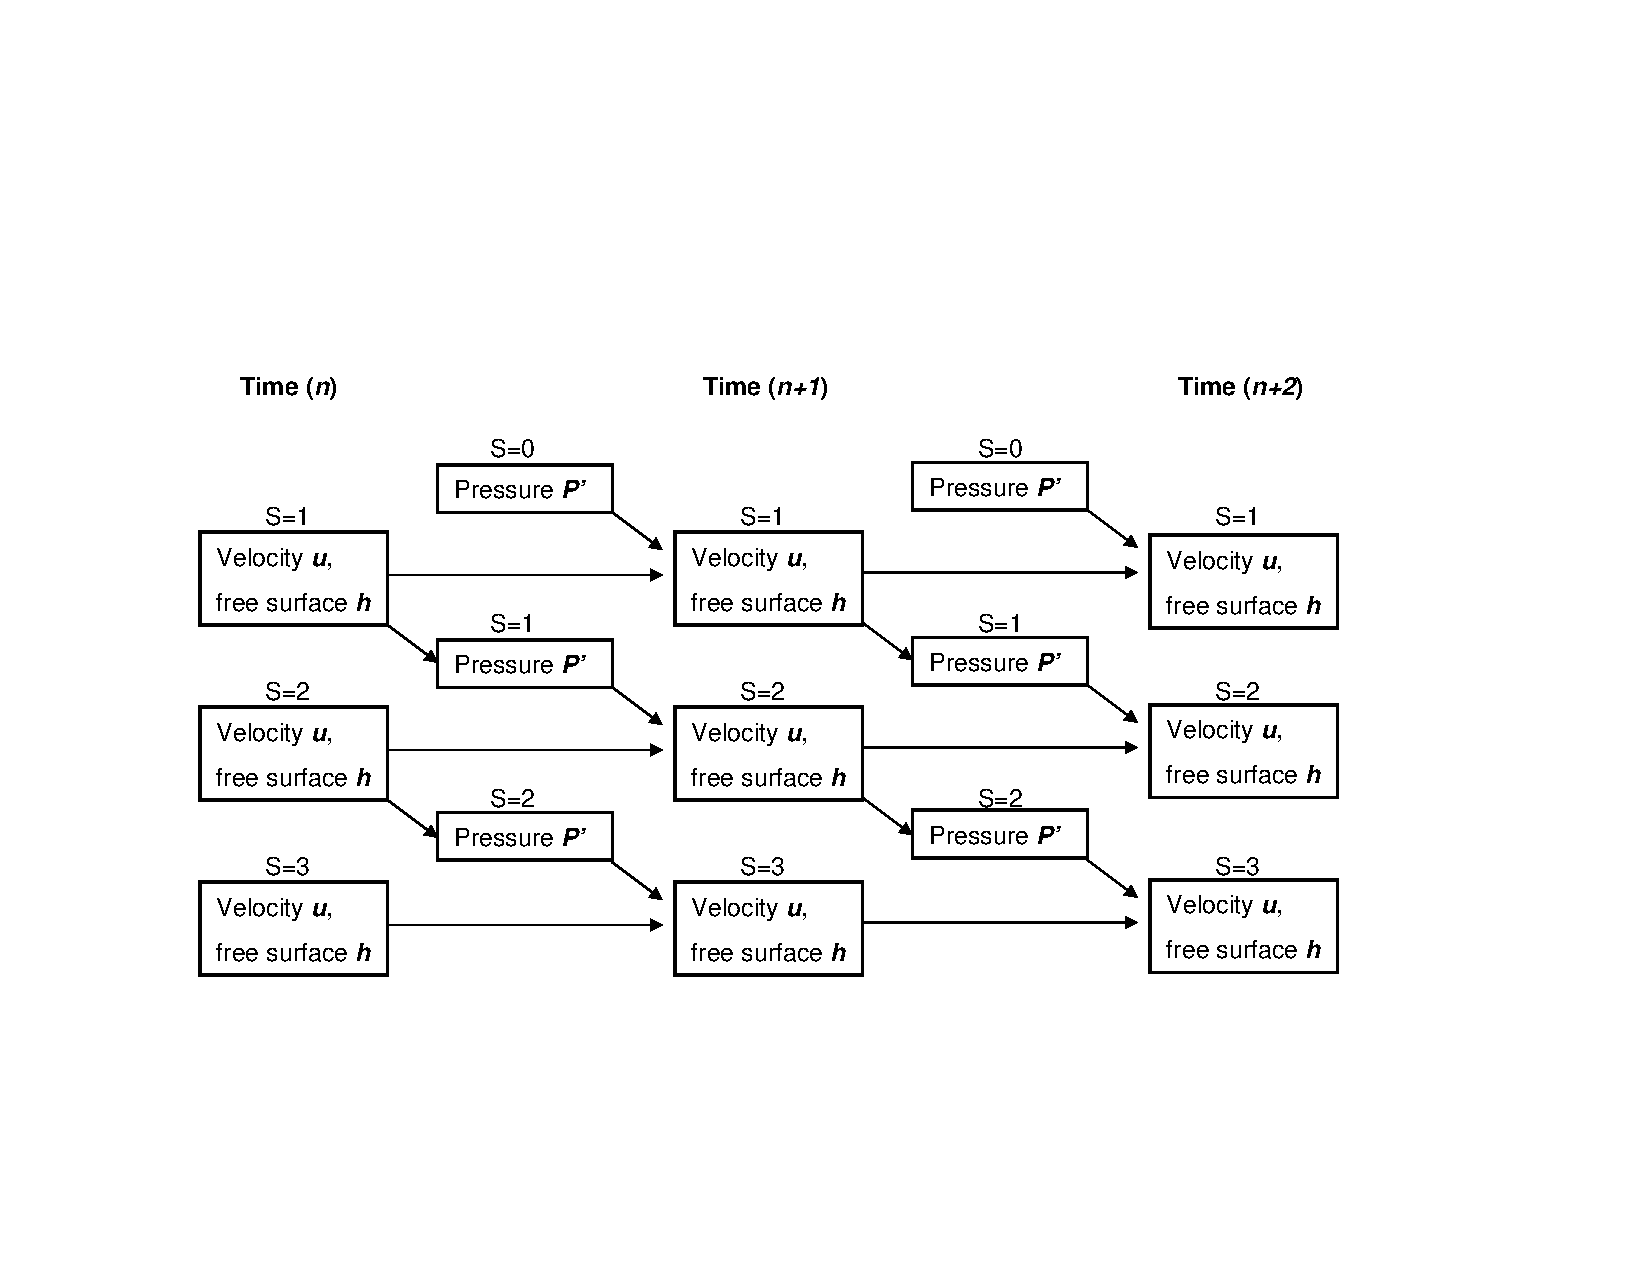
\includegraphics[width=5.5in]{../figures/SRM/SRM-chart.pdf}
    \caption{SRM iteration procedure}
    \label{fig:SRM-iteration}
  \end{center}
\end{figure}
\cp

\subsection{Standing Wave Test}

The numerical simulation of standing wave motion in a closed basin as mentioned in Chapter \ref{chapter:NumericalTest-StaWav} is performed to test the sequential regularization method for free-surface non-hydrostatic numerical model. The analytical approximation is documented by LeBlond \cite{LeBlond1978} and Jankowski \cite{Jankowski1999}.

\begin{equation}
\eta = A \cos(kx)\cos(\omega t)
\end{equation}
\begin{equation}
u=\omega A \frac{\cosh[k(z+d)]}{\sinh(kd)}\sin(kx)\sin(\omega t)
\end{equation}
\begin{equation}
w=-\omega A \frac{\sinh[k(z+d)]}{\sinh(kd)}\cos(kx)\sin(\omega t)
\end{equation}
\begin{equation}
C= \omega /k
\end{equation}
\begin{equation}
k=2 \pi/L
\end{equation}
\begin{equation}
\omega^2=gk \tanh(kd)
\end{equation}

In the numerical test, the length of the container is $L=10(m)$;
the equilibrium water depth is $d=10(m)$; the wave amplitude is
$A=0.1(m)$; the initial free surface is specified as $\eta_0 = A
cos(kx)$; the celerity of the wave is $C= \sqrt{\frac{gL}{2
\pi}tanh \frac{2 \pi h}{L}}=5.575 (m/s)$; and the period of the
oscillation is: $ T=2L/C= 3.587 (s)$. In the numerical simulation, $\Delta x = 0.5 (m)$, $\Delta z = 0.25 (m)$, $\Delta t = T/800$, and the viscosity is set to zero. The under-relaxation parameter is tested with $\beta=1$, and the penalty parameter is $\epsilon=200$.
The numerical results and analytical solutions of velocity and pressure at $t=1/8T$, $t=1/2T$, and $t=5/8T$ are plotted in Figure \ref{fig:SRM-StanWav-1-8}, \ref{fig:SRM-StanWav-4-8}, and \ref{fig:SRM-StanWav-5-8}. The free surface level at $x=0.25(m)$ and $x=9.75(m)$ are shown in Figure \ref{fig:elevation_x025_SRM_cropped_bottom24} and \ref{fig:elevation_x975_SRM_cropped_bottom24}. The velocity $u$ versus time is shown in Figure \ref{fig:U_X25_Z5_SRM_cropped_bottom24}.

\begin{figure}
%\vspace{-0.15in}
\hspace{0.0in}
\subfigure[Sequential regularization method] % caption for subfigure a
{
    \label{fig:SRM-StanWav-1-8-SRM}
    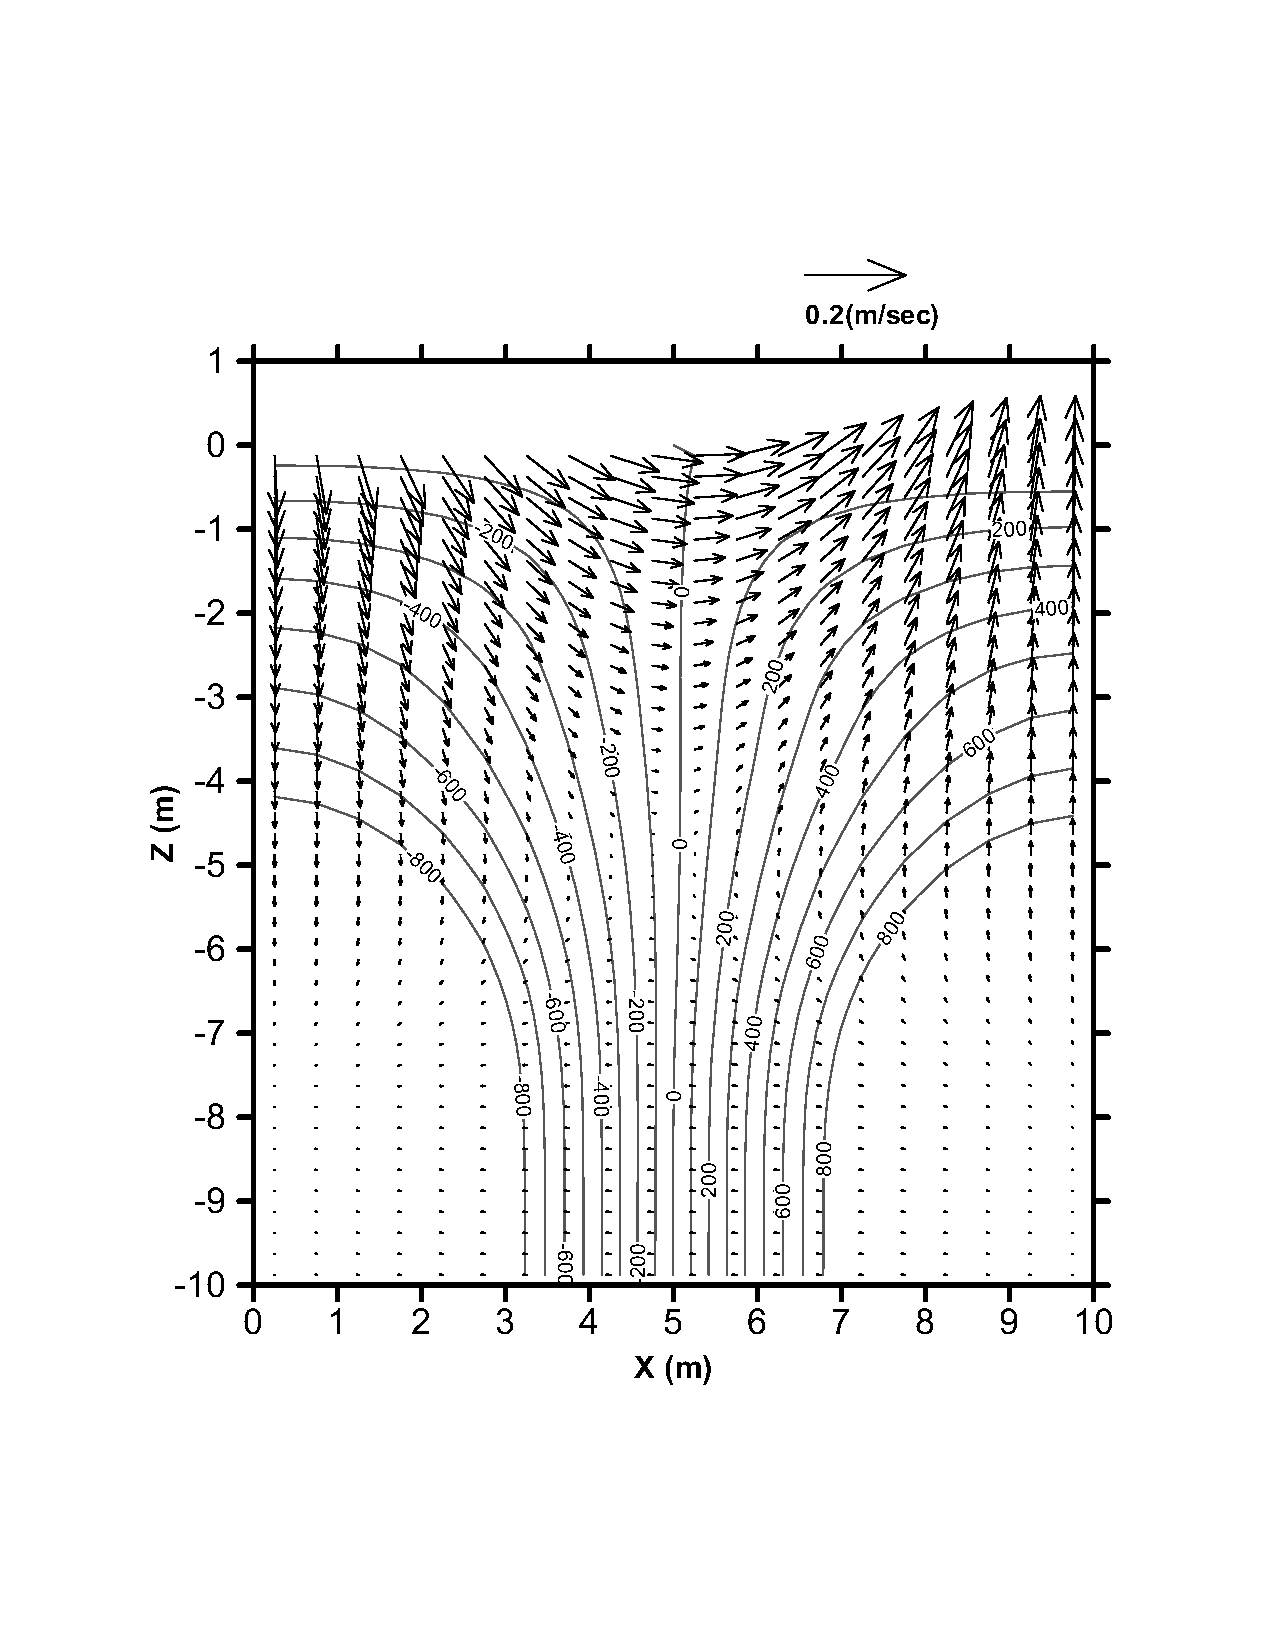
\includegraphics[width=2.675in]{../figures/SRM/SRM_StandingWave_1-8.pdf}

}
\hspace{-0.2in}
\subfigure[Analytical solution] % caption for subfigure b
{
    \label{fig:SRM-StanWav-1-8-Ana}
    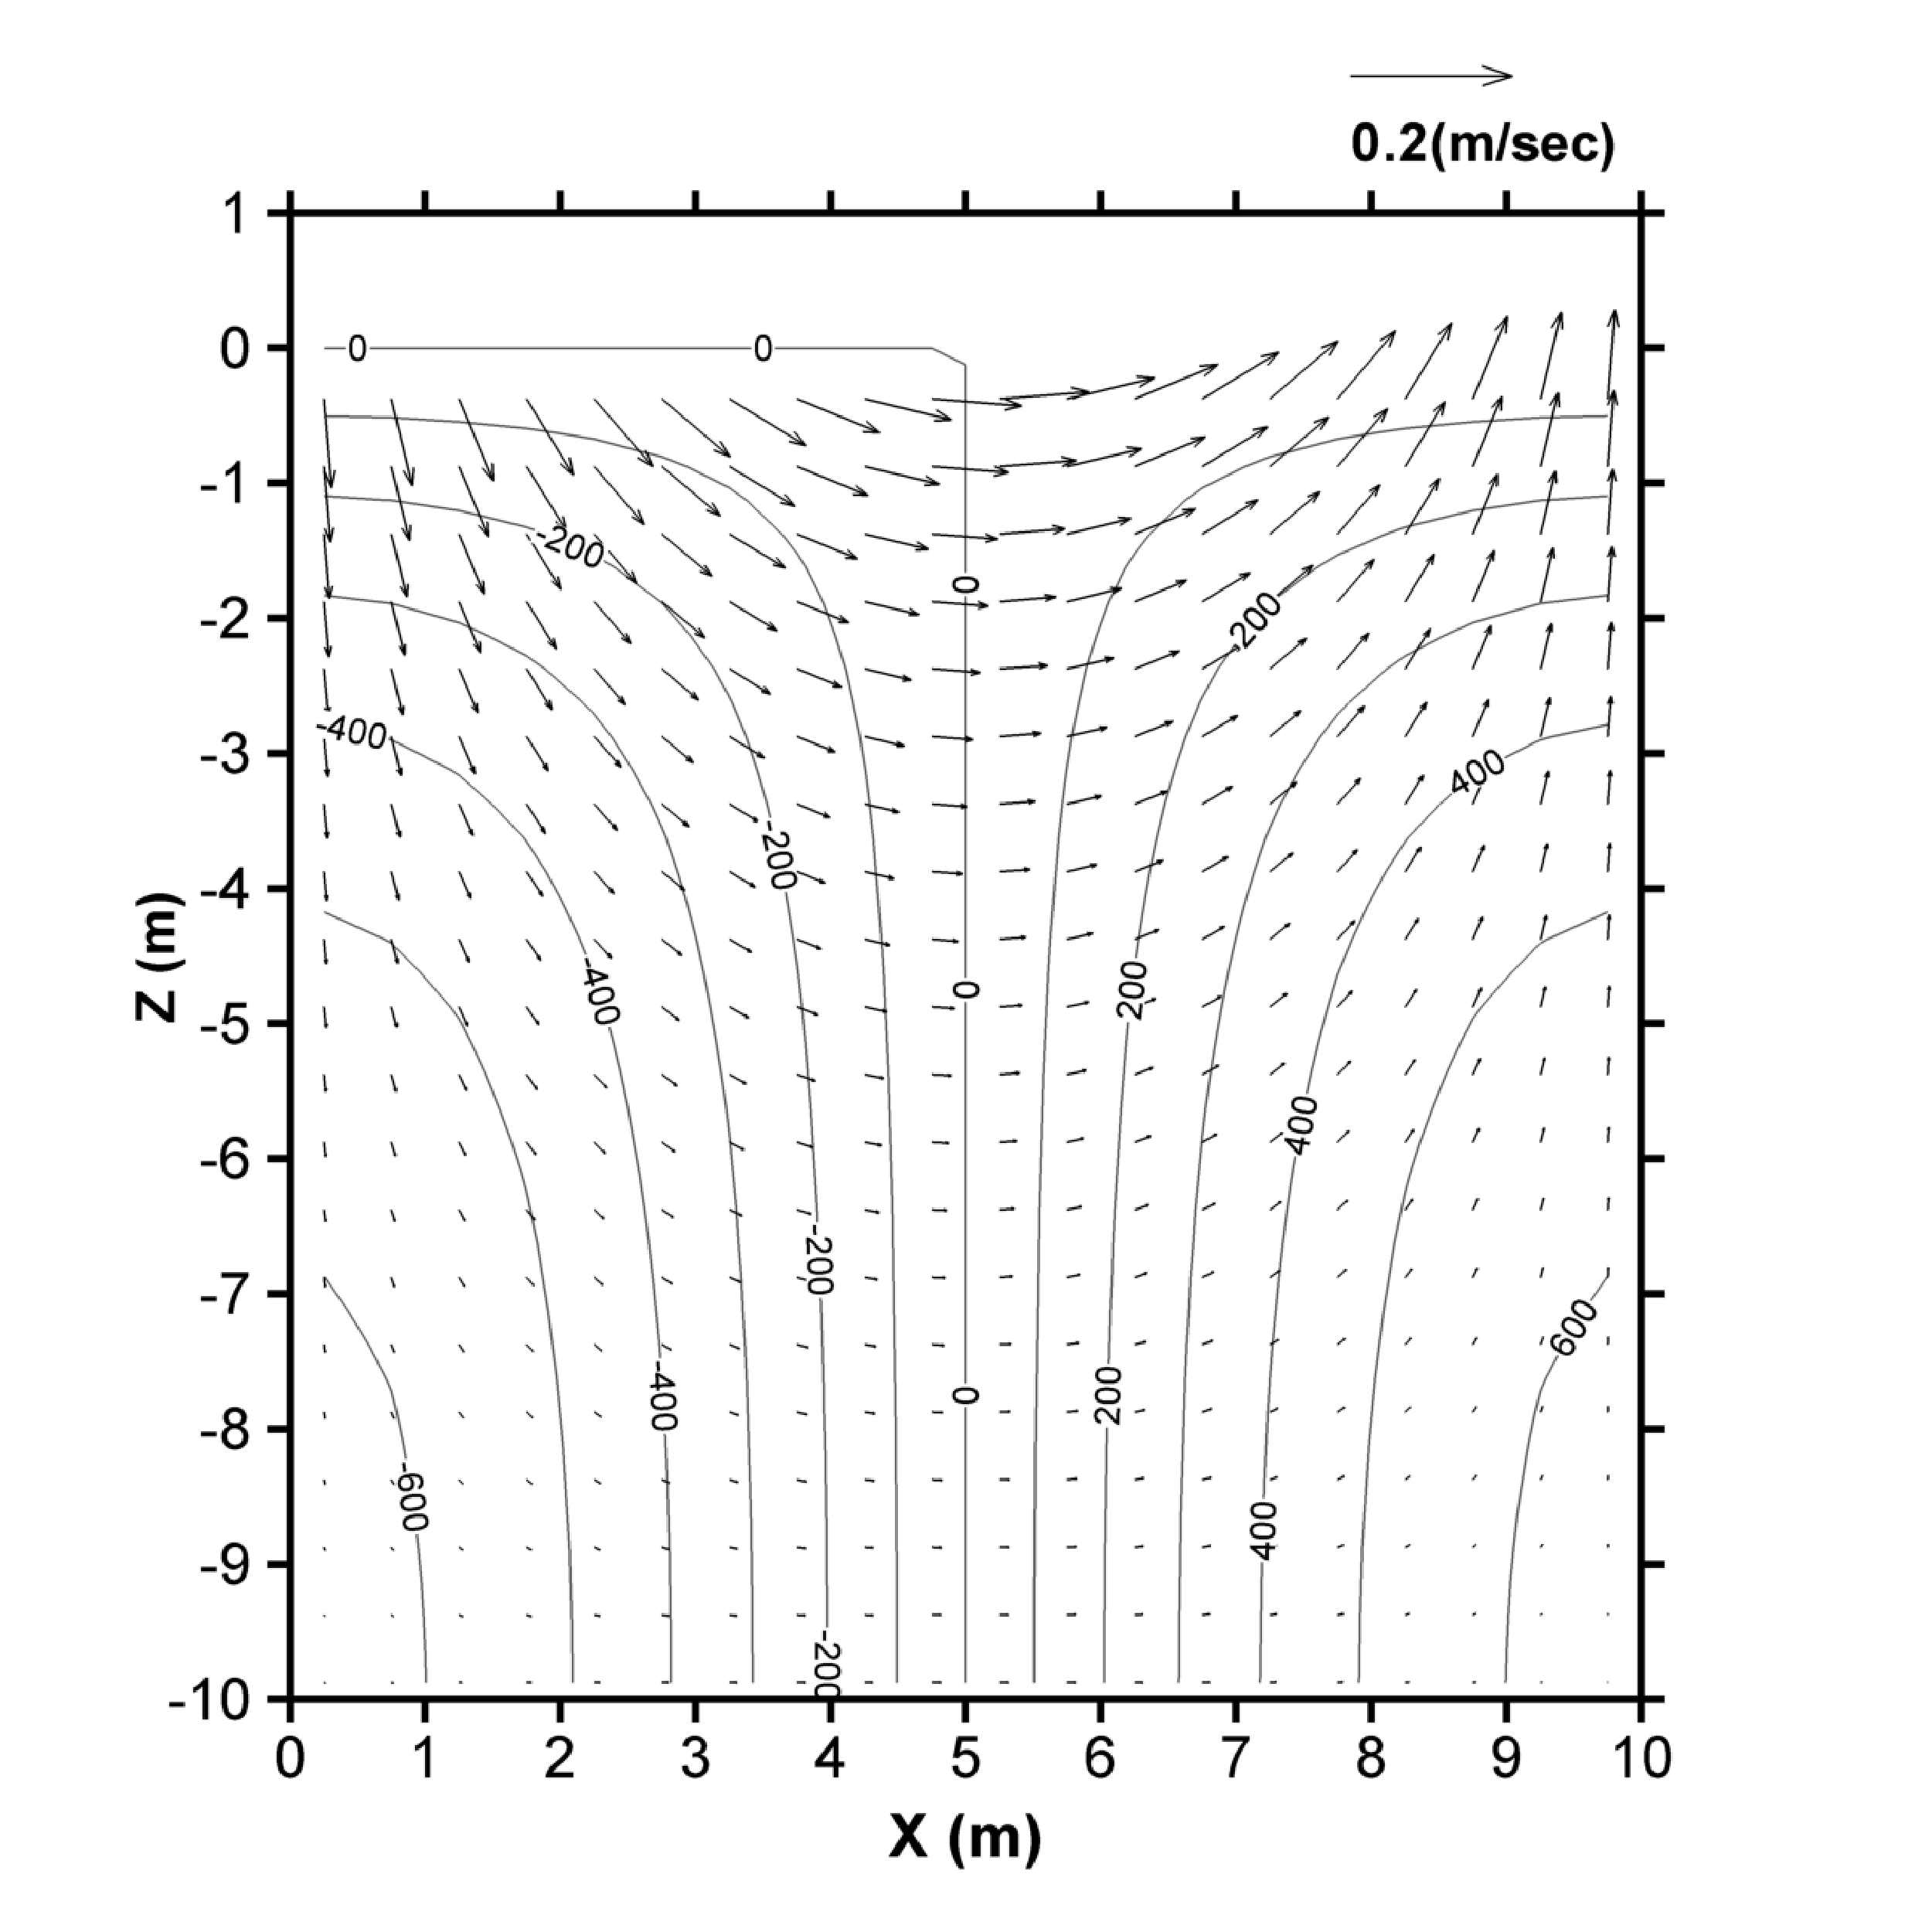
\includegraphics[width=3.2in]{../figures/StanWav/StanWav-Ana-1-8.pdf}
}
\caption{Standing wave test. Pressure and velocity plots at $t= 1/8 T$}
\label{fig:SRM-StanWav-1-8}
\vspace{0.3in}

\hspace{0.0in}
\subfigure[Sequential regularization method] % caption for subfigure a
{
    \label{fig:SRM-StanWav-4-8-SRM}
    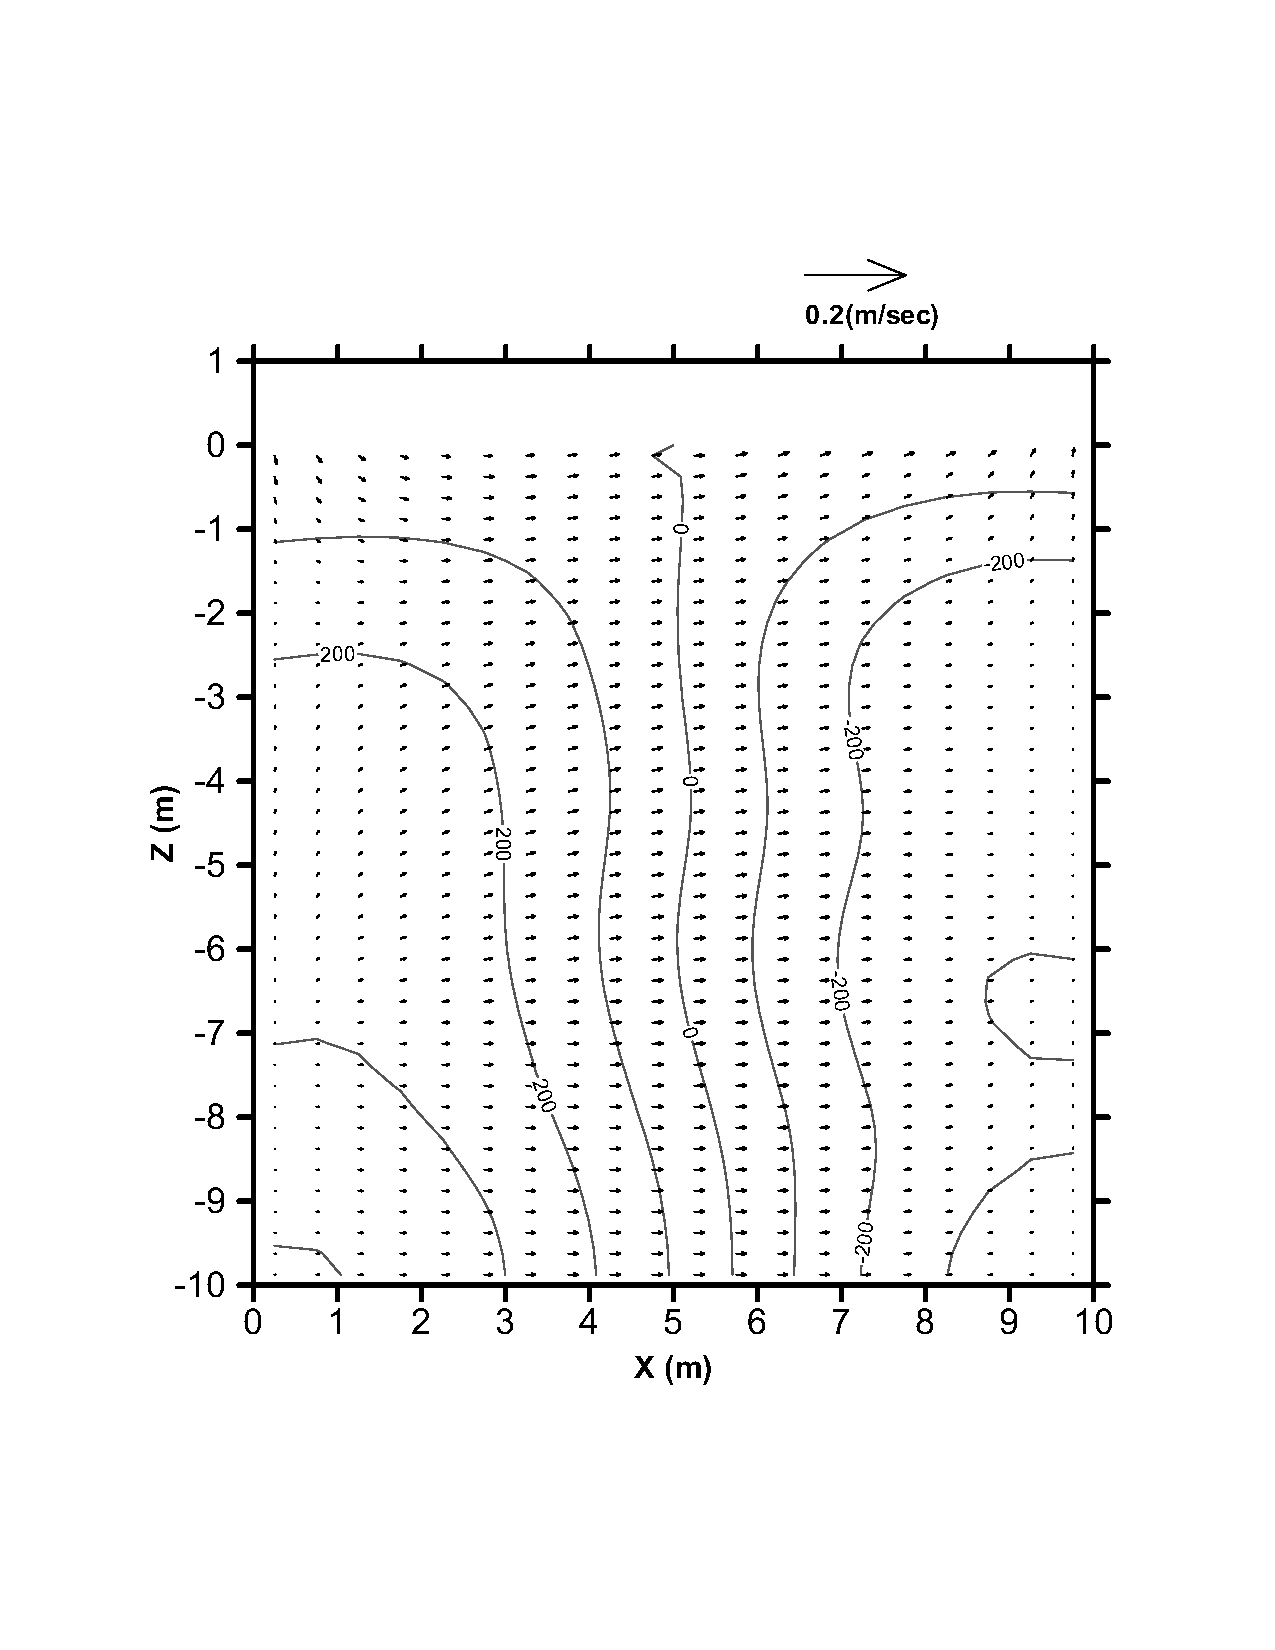
\includegraphics[width=2.675in]{../figures/SRM/SRM_StandingWave_4-8.pdf}
}
\hspace{-0.2in}
\subfigure[Analytical solution] % caption for subfigure b
{
    \label{fig:SRM-StanWav-4-8-Ana}
    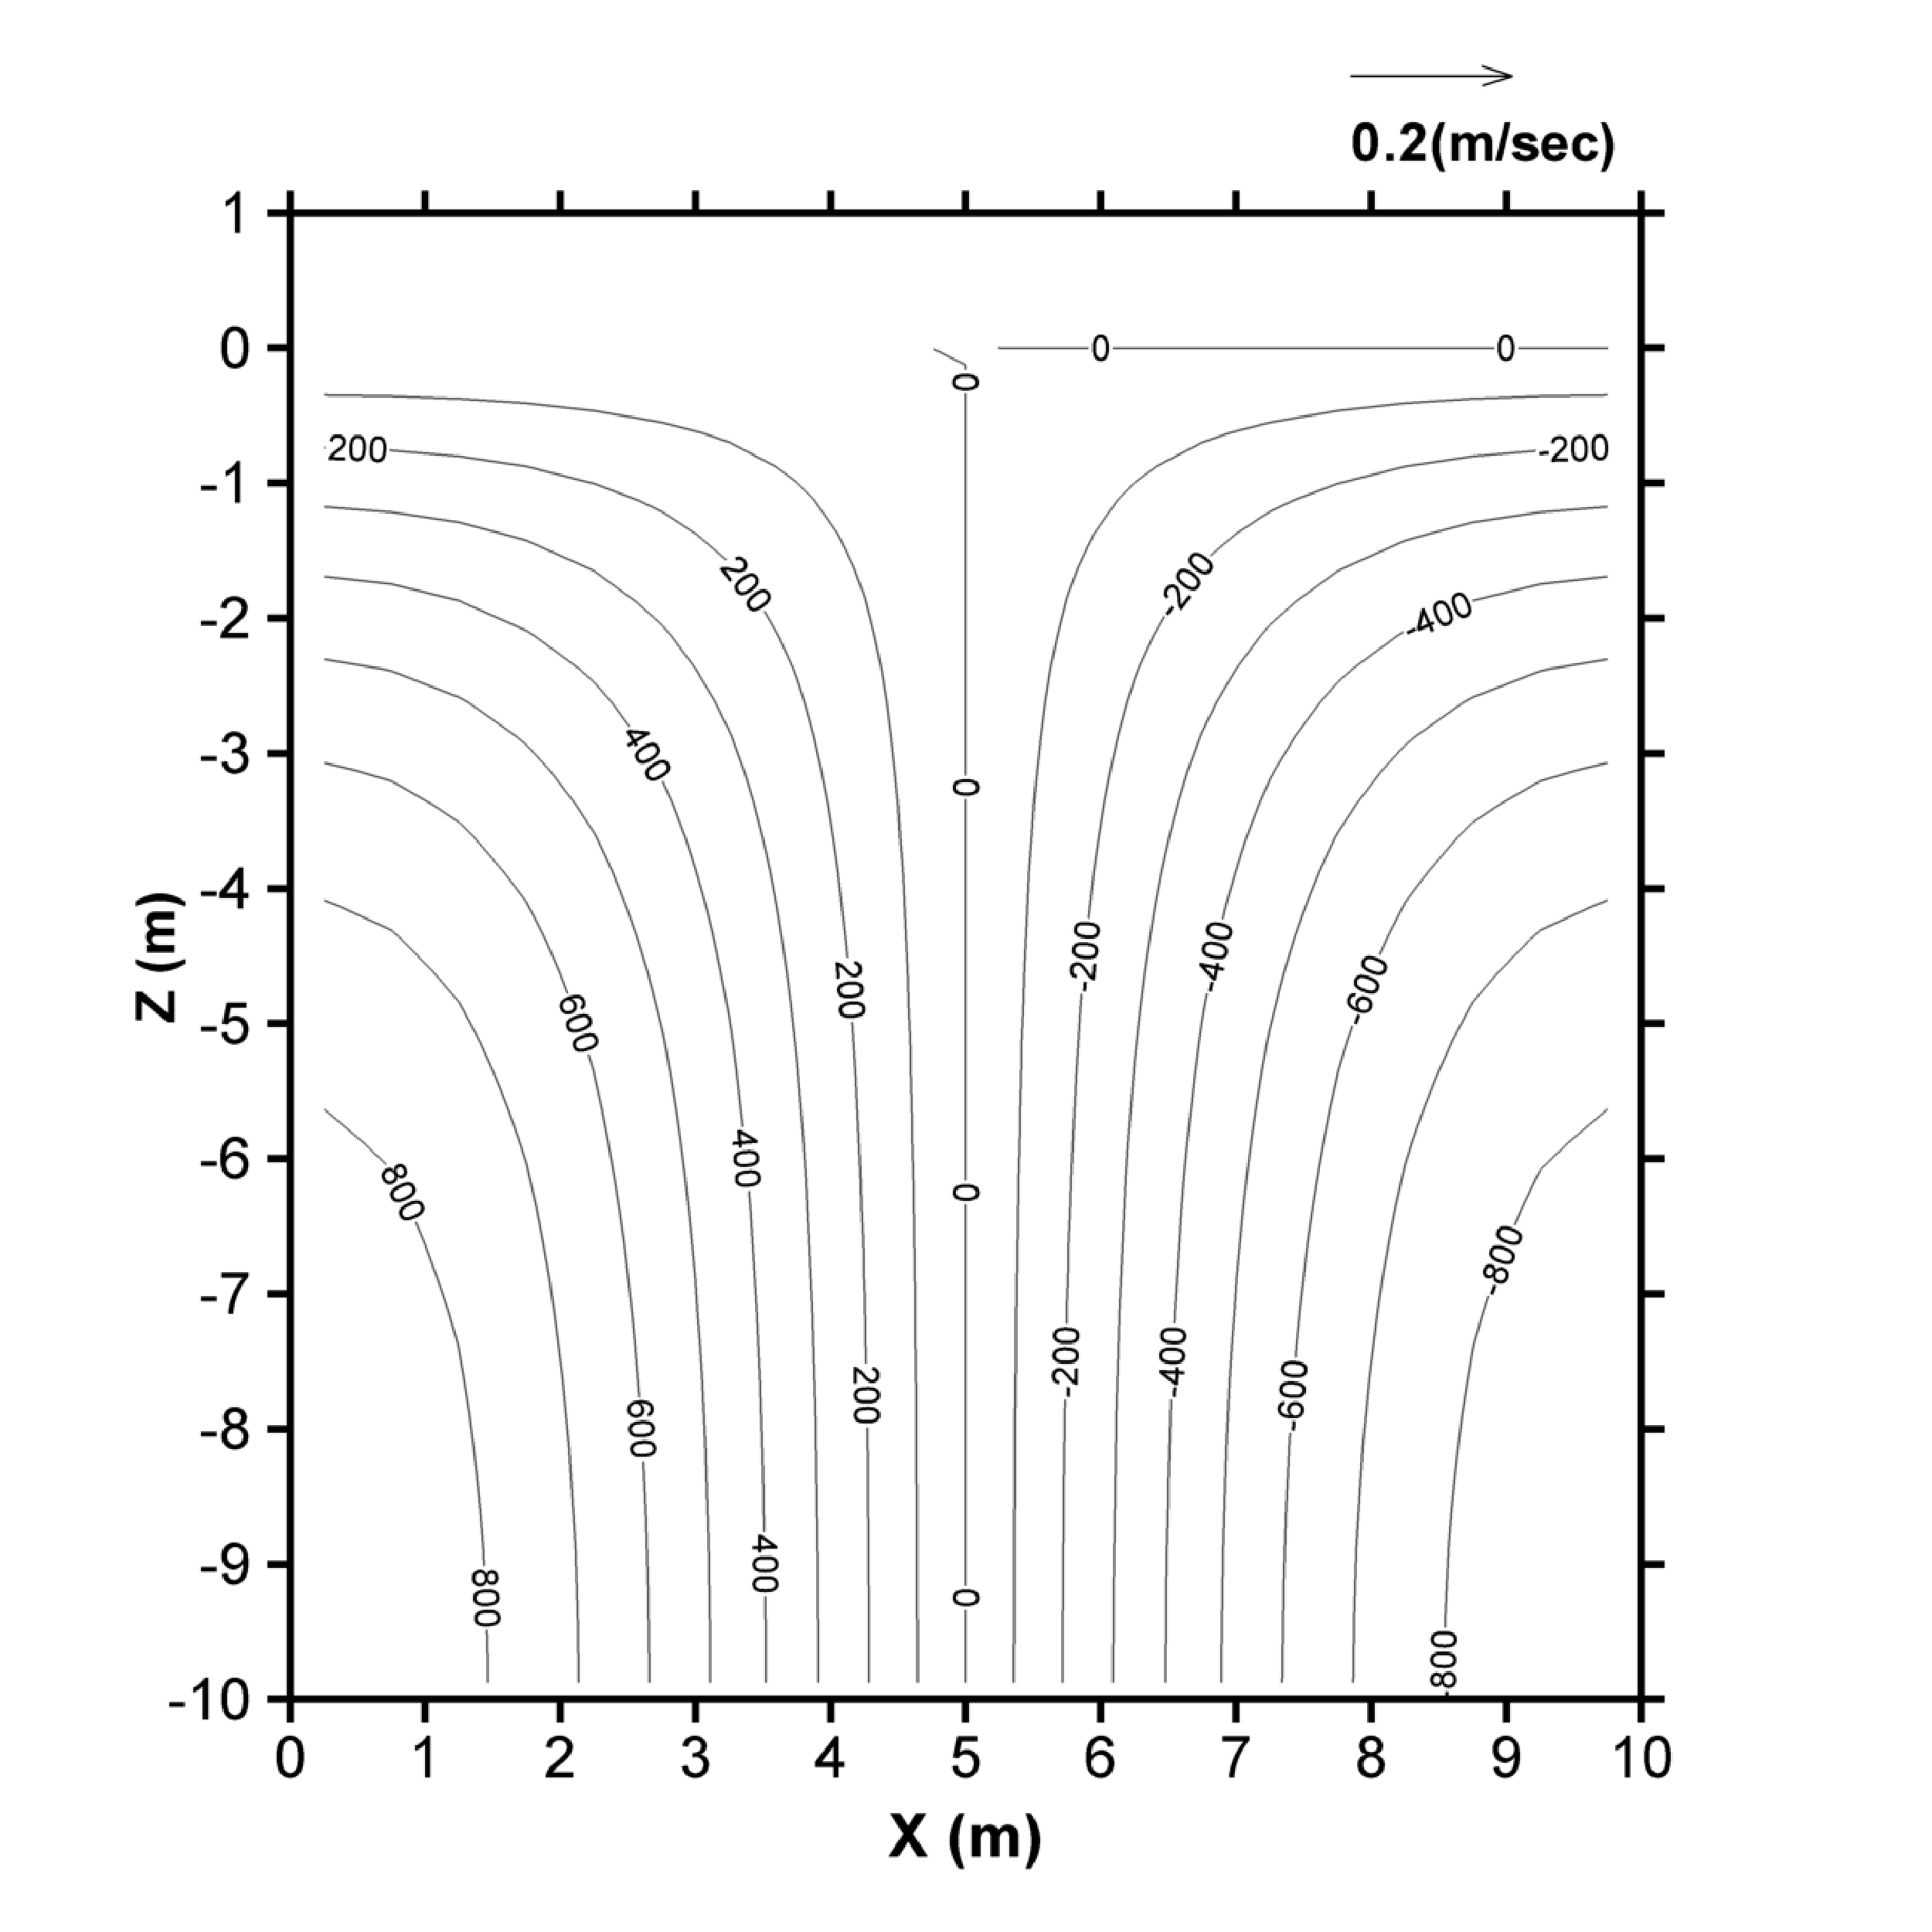
\includegraphics[width=3.2in]{../figures/StanWav/StanWav-Ana-4-8.pdf}
}
\caption{Standing wave test. Pressure and velocity plots at $t= 1/2 T$}
\label{fig:SRM-StanWav-4-8}
\end{figure}



\begin{figure}[htbp]
\vspace{-0.2in}
\hspace{0.0in}
\subfigure[Sequential regularization method] % caption for subfigure a
{
    \label{fig:SRM-StanWav-1-8-SRM}
    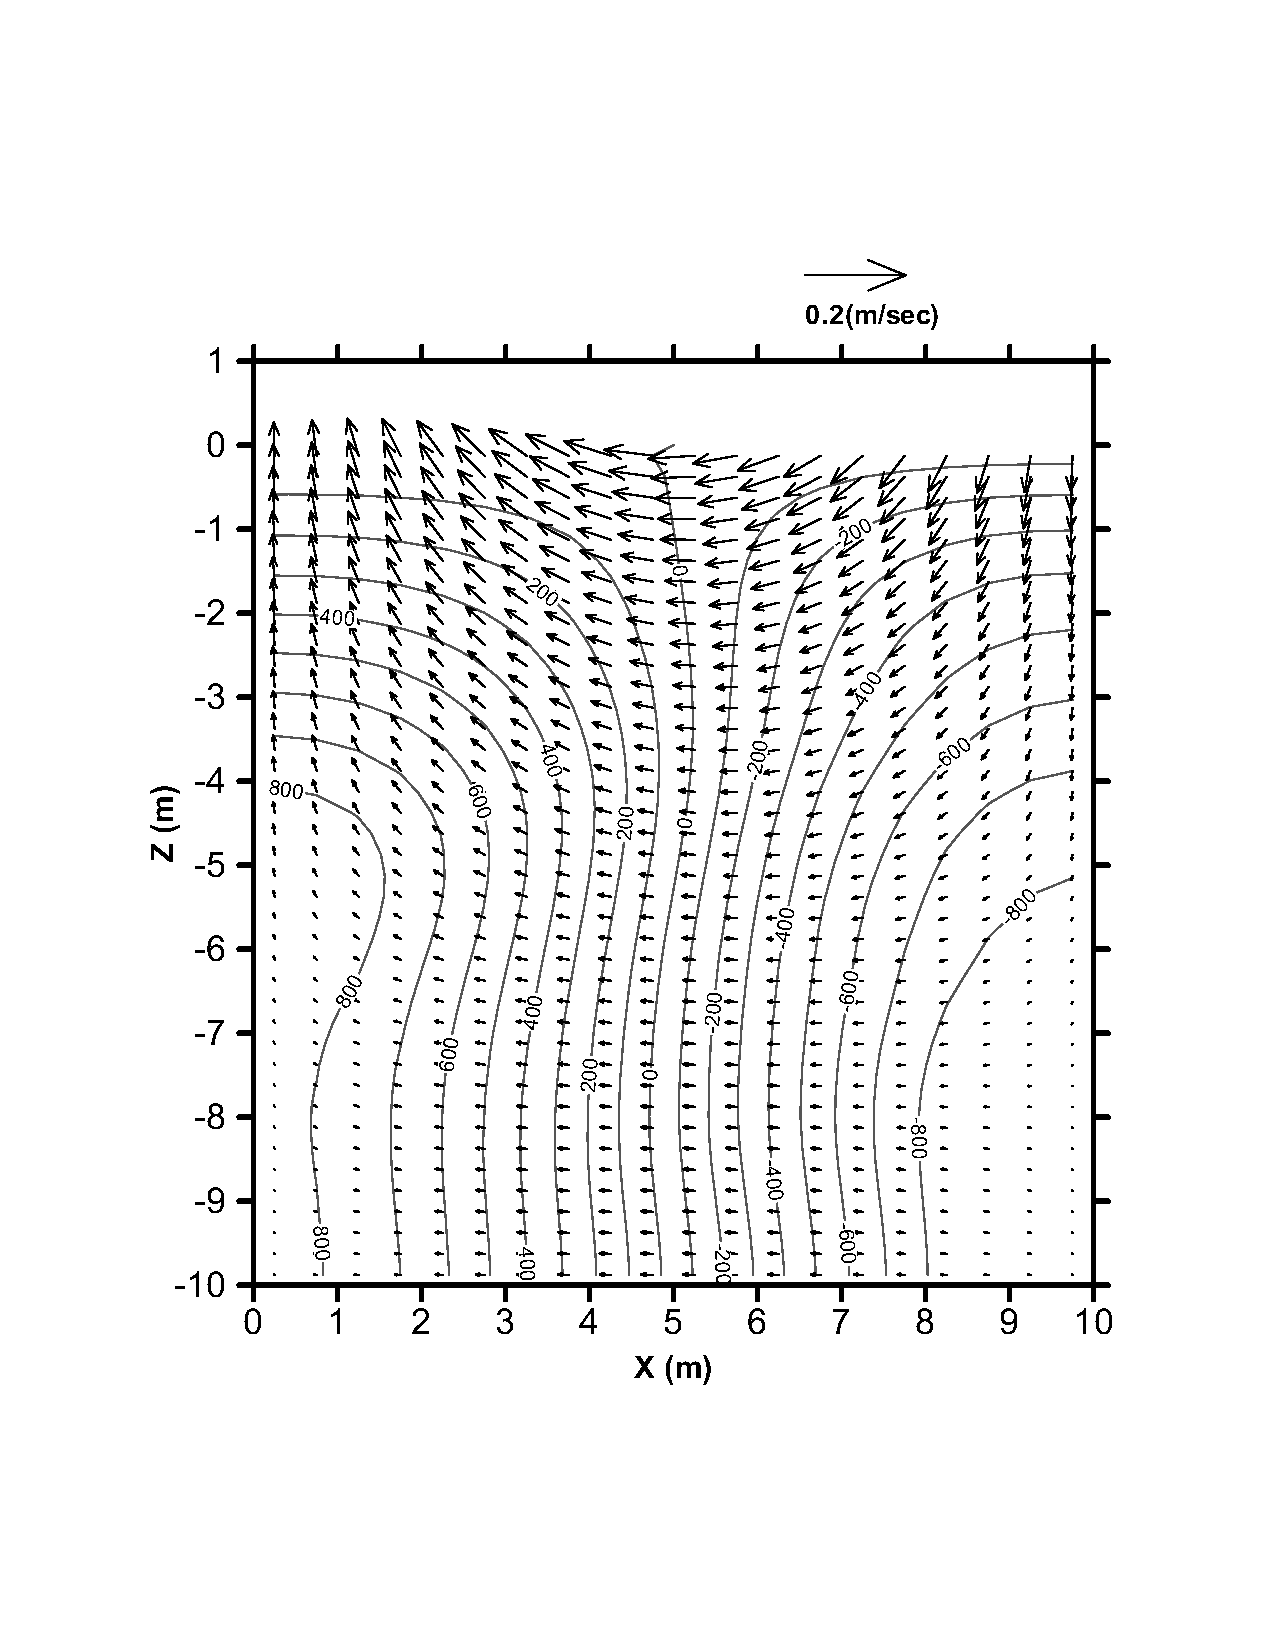
\includegraphics[width=2.675in]{../figures/SRM/SRM_StandingWave_5-8.pdf}
}
\hspace{-0.2in}
\subfigure[Analytical solution] % caption for subfigure b
{
    \label{fig:SRM-StanWav-1-8-Ana}
    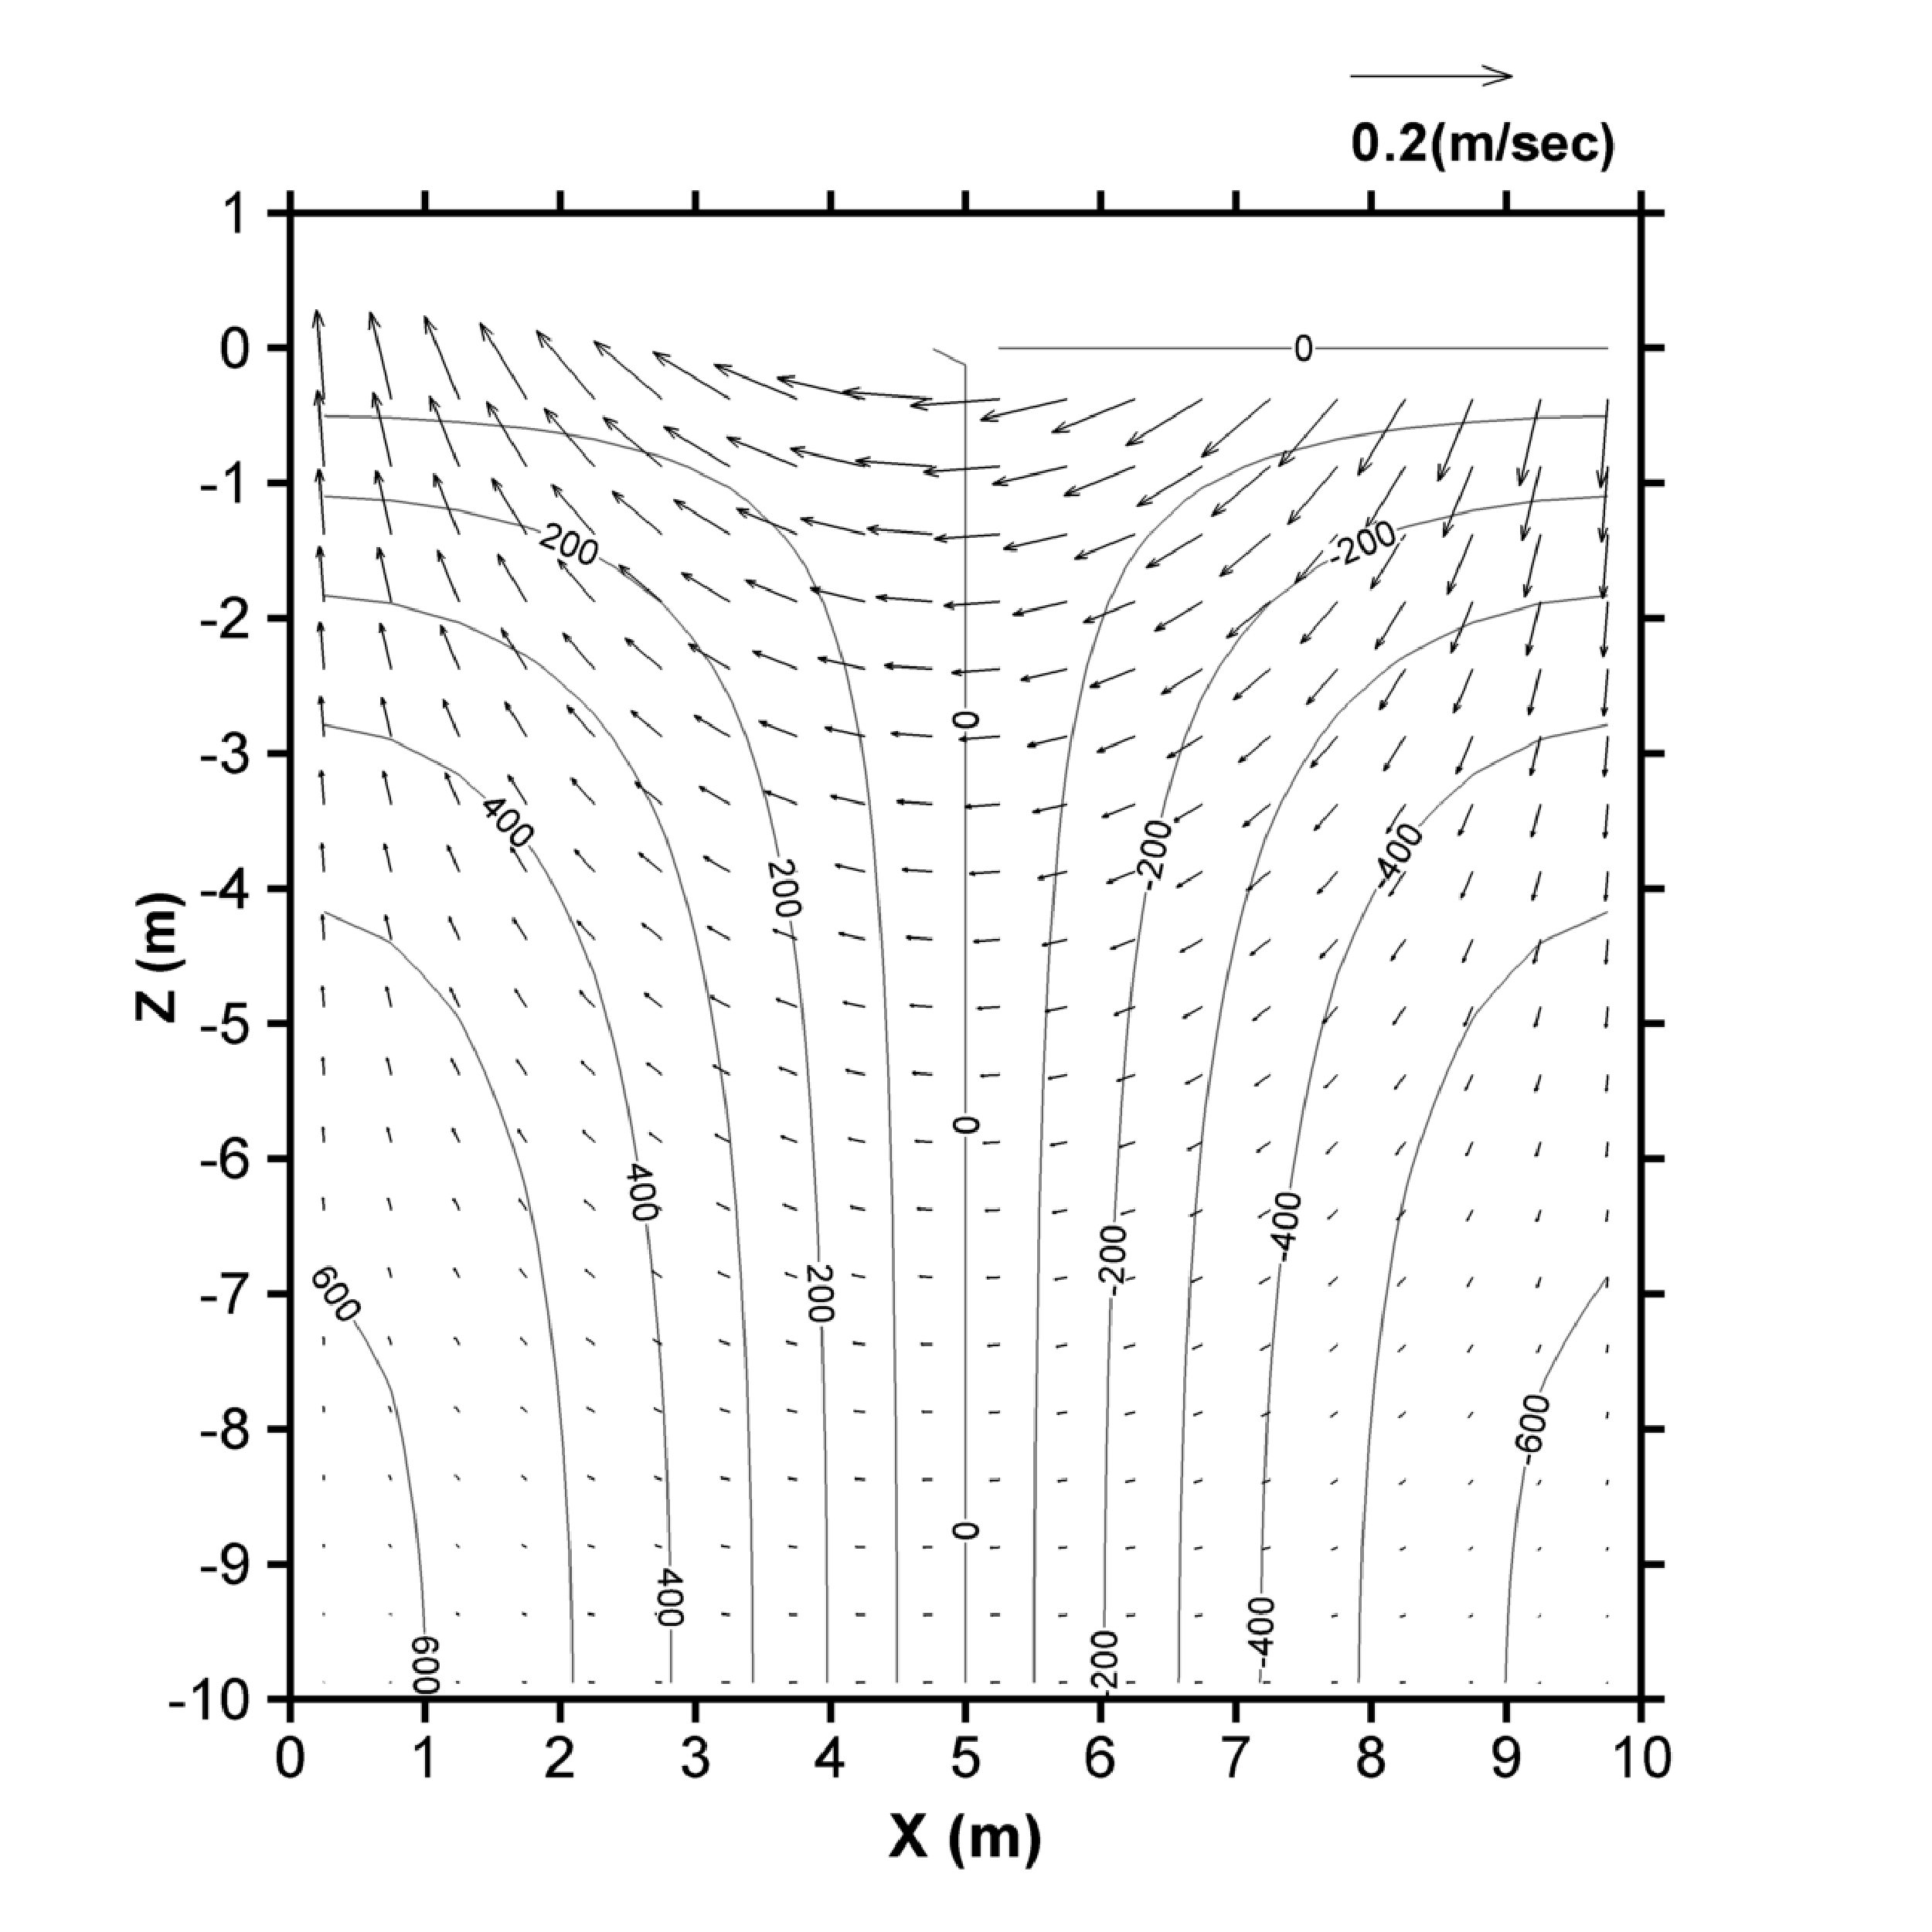
\includegraphics[width=3.2in]{../figures/StanWav/StanWav-Ana-5-8.pdf}
}
\caption{Standing wave test. Pressure and velocity plots at $t= 5/8 T$}
\label{fig:SRM-StanWav-5-8} % caption for the whole figure

\vspace{0.9in}
\hspace{0.3in}
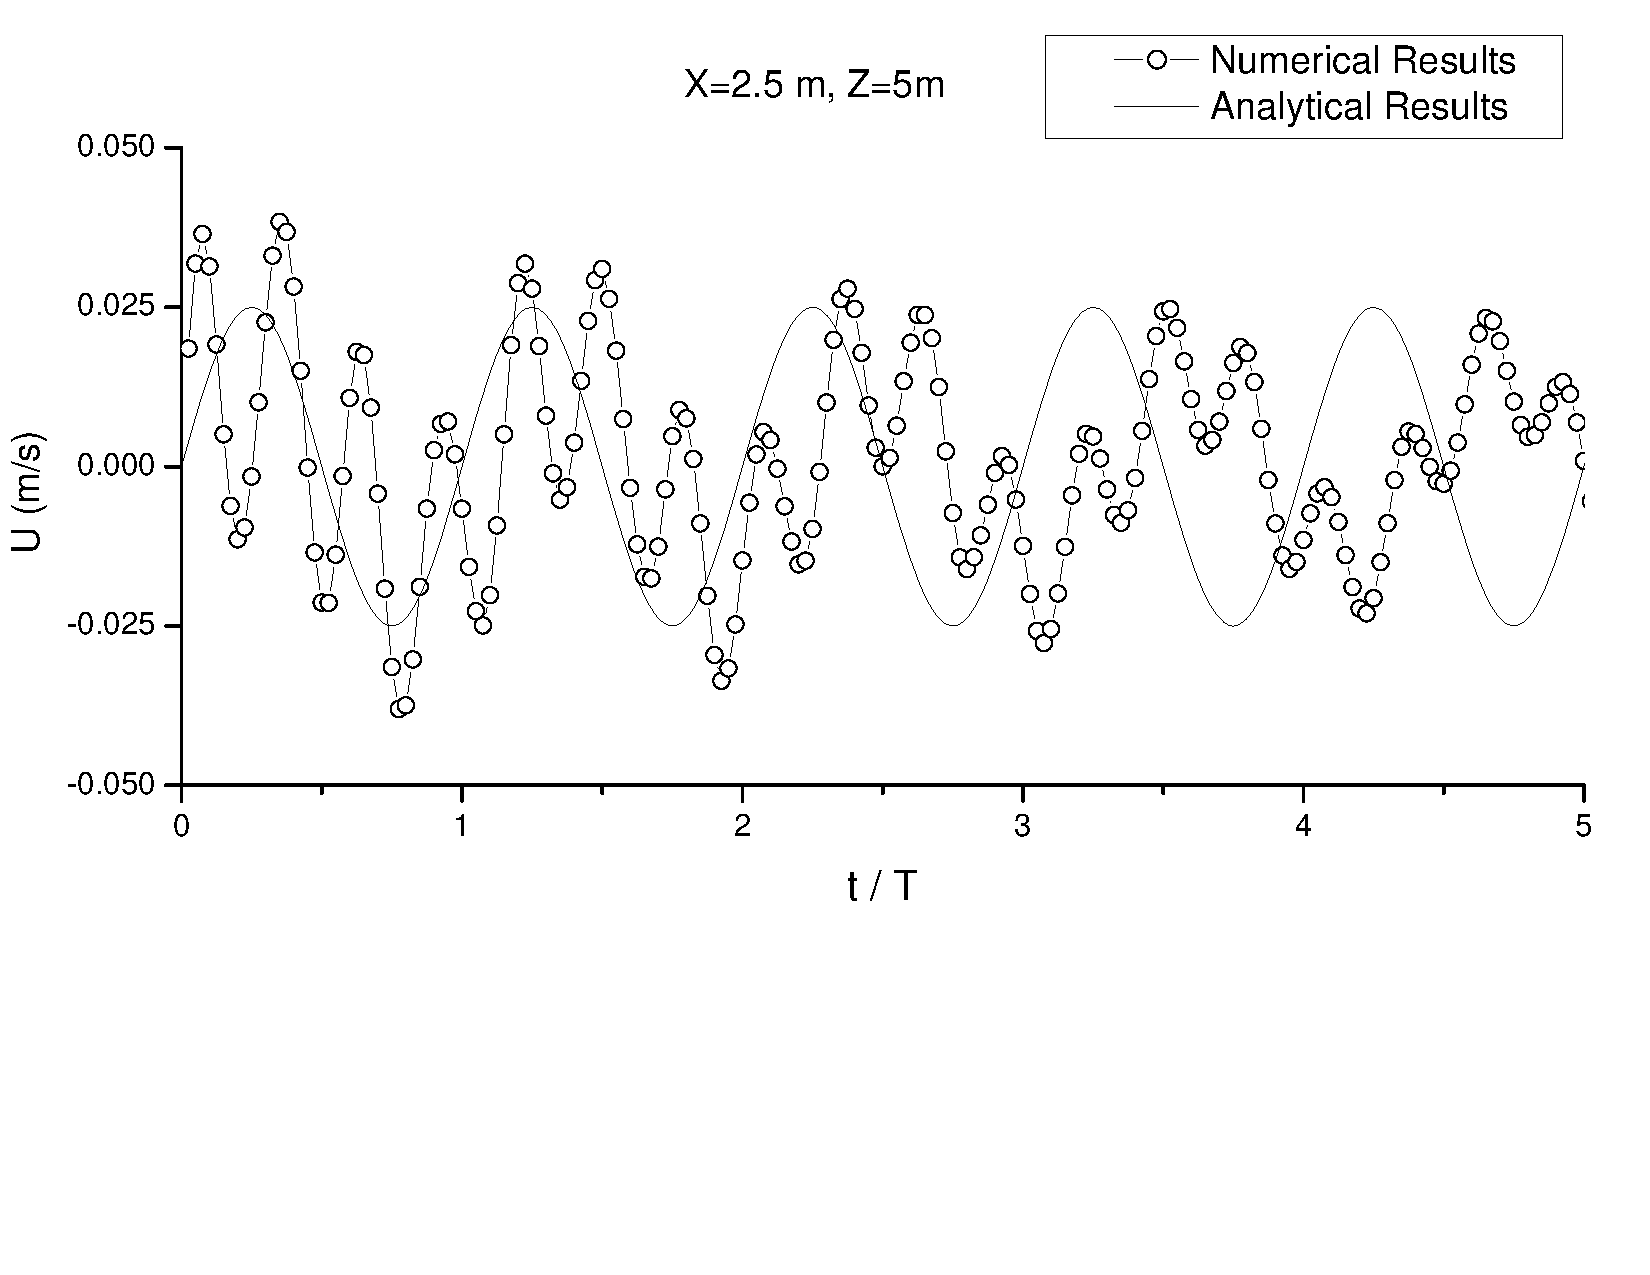
\includegraphics[scale=0.45]{../figures/SRM/U_X25_Z5_SRM_cropped_bottom24.pdf}
\label{fig:U_X25_Z5_SRM_cropped_bottom24}
\caption{Standing wave test. Velocity $u$ versus time}
\end{figure}


\begin{figure}[h]

\vspace{0.1in}
\hspace{0.3in}
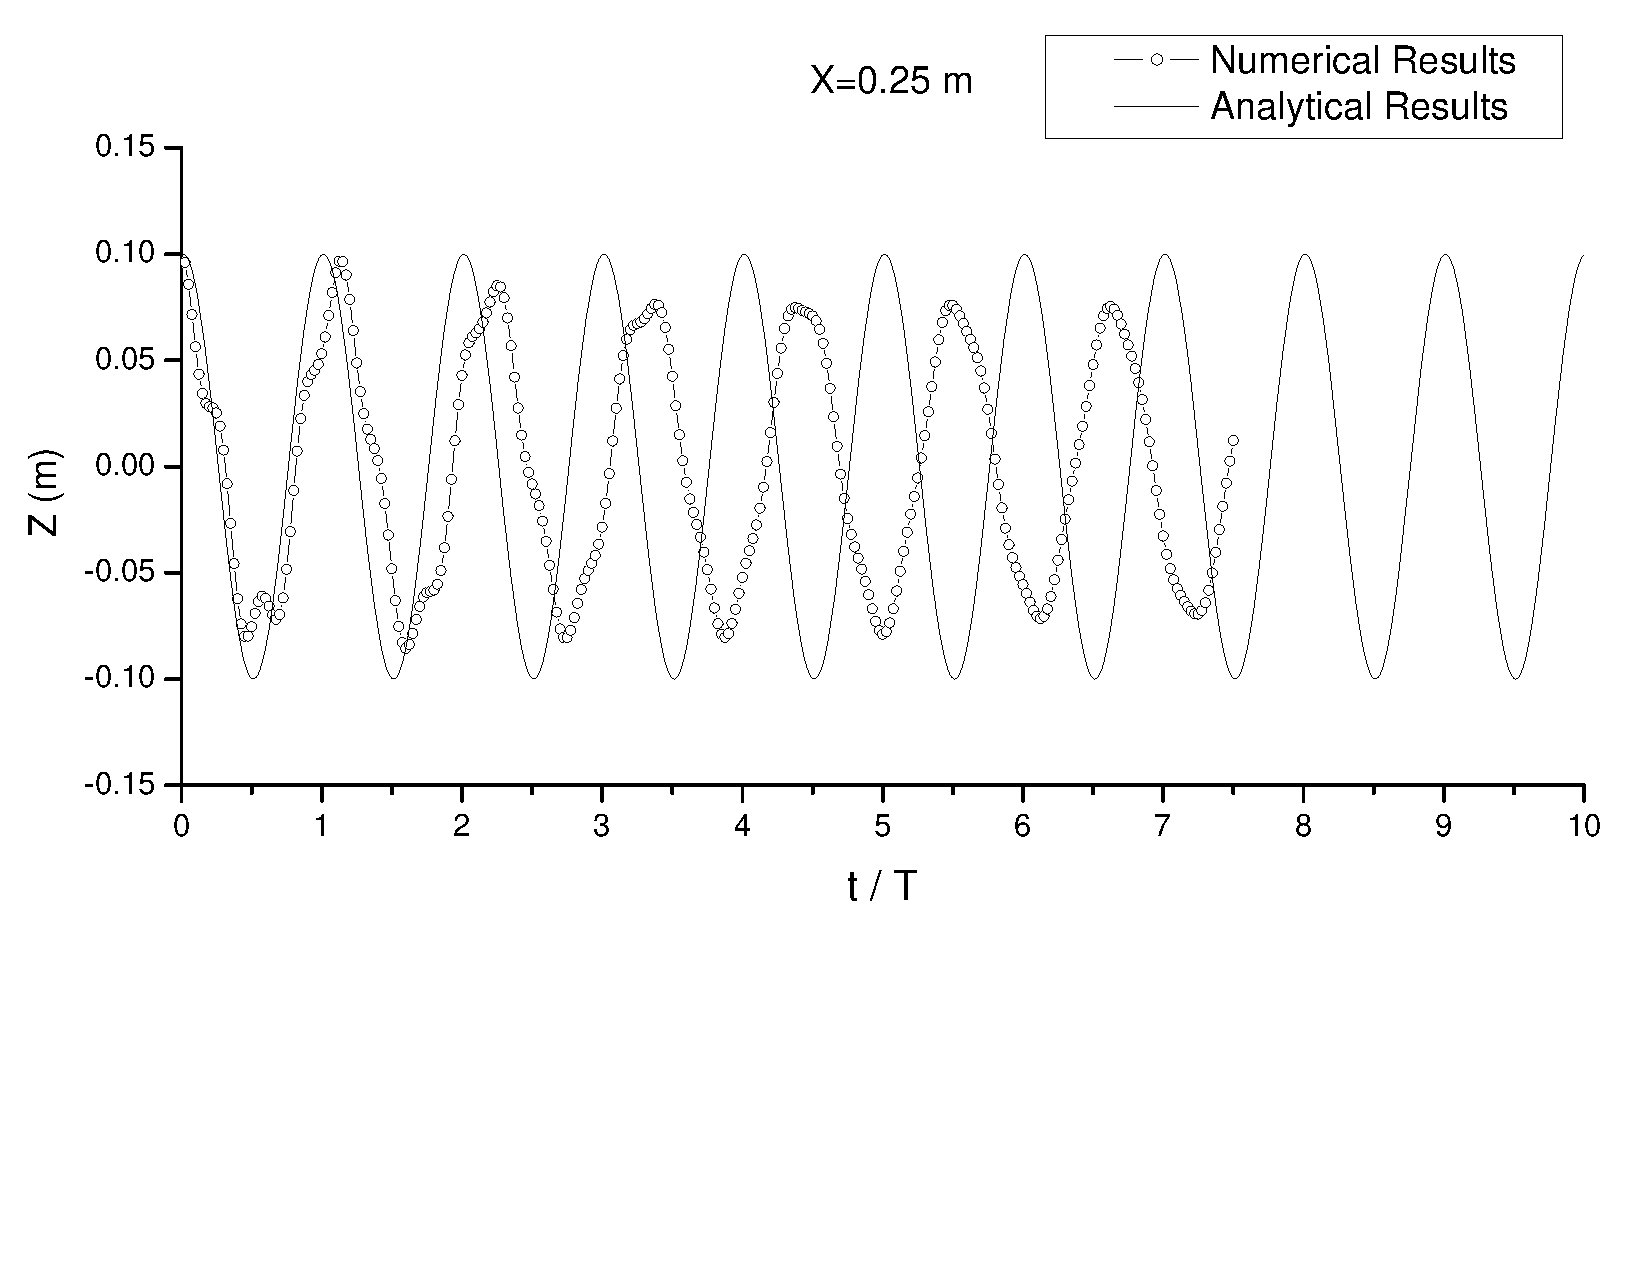
\includegraphics[scale=0.45]{../figures/SRM/elevation_x025_SRM_cropped_bottom24.pdf}
\label{fig:elevation_x025_SRM_cropped_bottom24}
\caption{Standing wave test. Elevation versus time}


\vspace{0.9in}
\hspace{0.3in}
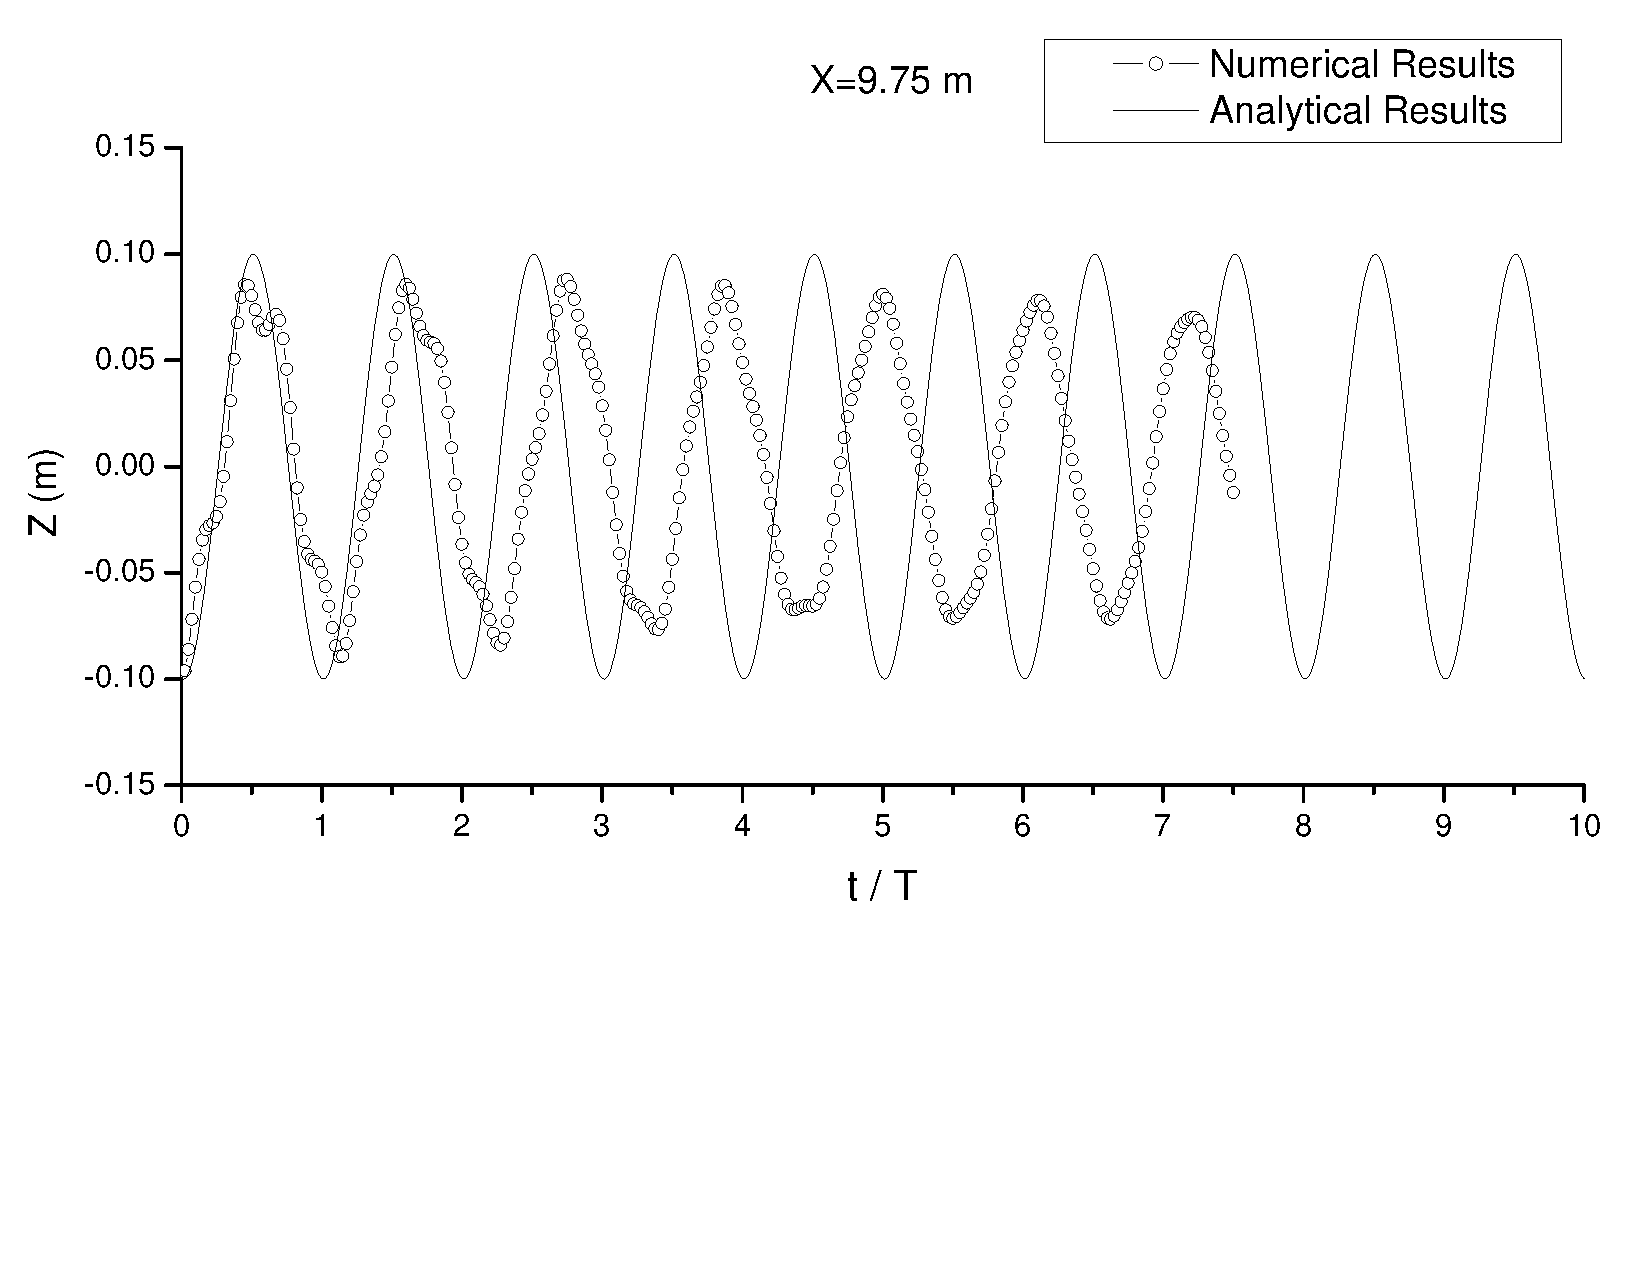
\includegraphics[scale=0.45]{../figures/SRM/elevation_x975_SRM_cropped_bottom24.pdf}
\label{fig:elevation_x975_SRM_cropped_bottom24}
\caption{Standing wave test. Surface elevation versus time}
\end{figure}

\cp

\section{Domain Decomposition with Sequential Regularization Method}

The explicit sequential regularization method is proposed for the domain decomposition. The subdomain interface is computed with the SRM with the subdomains modeled with implicit non-hydrostatic numerical methods. This idea of mixing explicit and implicit numerical methods is extended from the common technique of using forward Euler on even nodes and backward Euler on odd nodes. The advantage of the combination of explicit and implicit methods is that the parallel computation is straightforward on the explicit subdomain boundaries and the quality of stability is retained within implicit subdomains. Amitai et. al. \cite{amitai1998} applied this concept on domain decomposition for
parabolic partial differential equations, where the subdomain boundaries are approximated with Green's function. A diffusion problem is also demonstrated to show the feasibility.

The concept of the domain decomposition with SRM is shown in Figure \ref{fig:SRM-DDM}. The subdomain B has a smaller time step and higher spatial resolution than subdomain A. The boundary conditions for subdomains are computed by the SRM method, which uses the smallest time step and the highest spatial resolution.
\begin{figure}[h]
  \begin{center}
    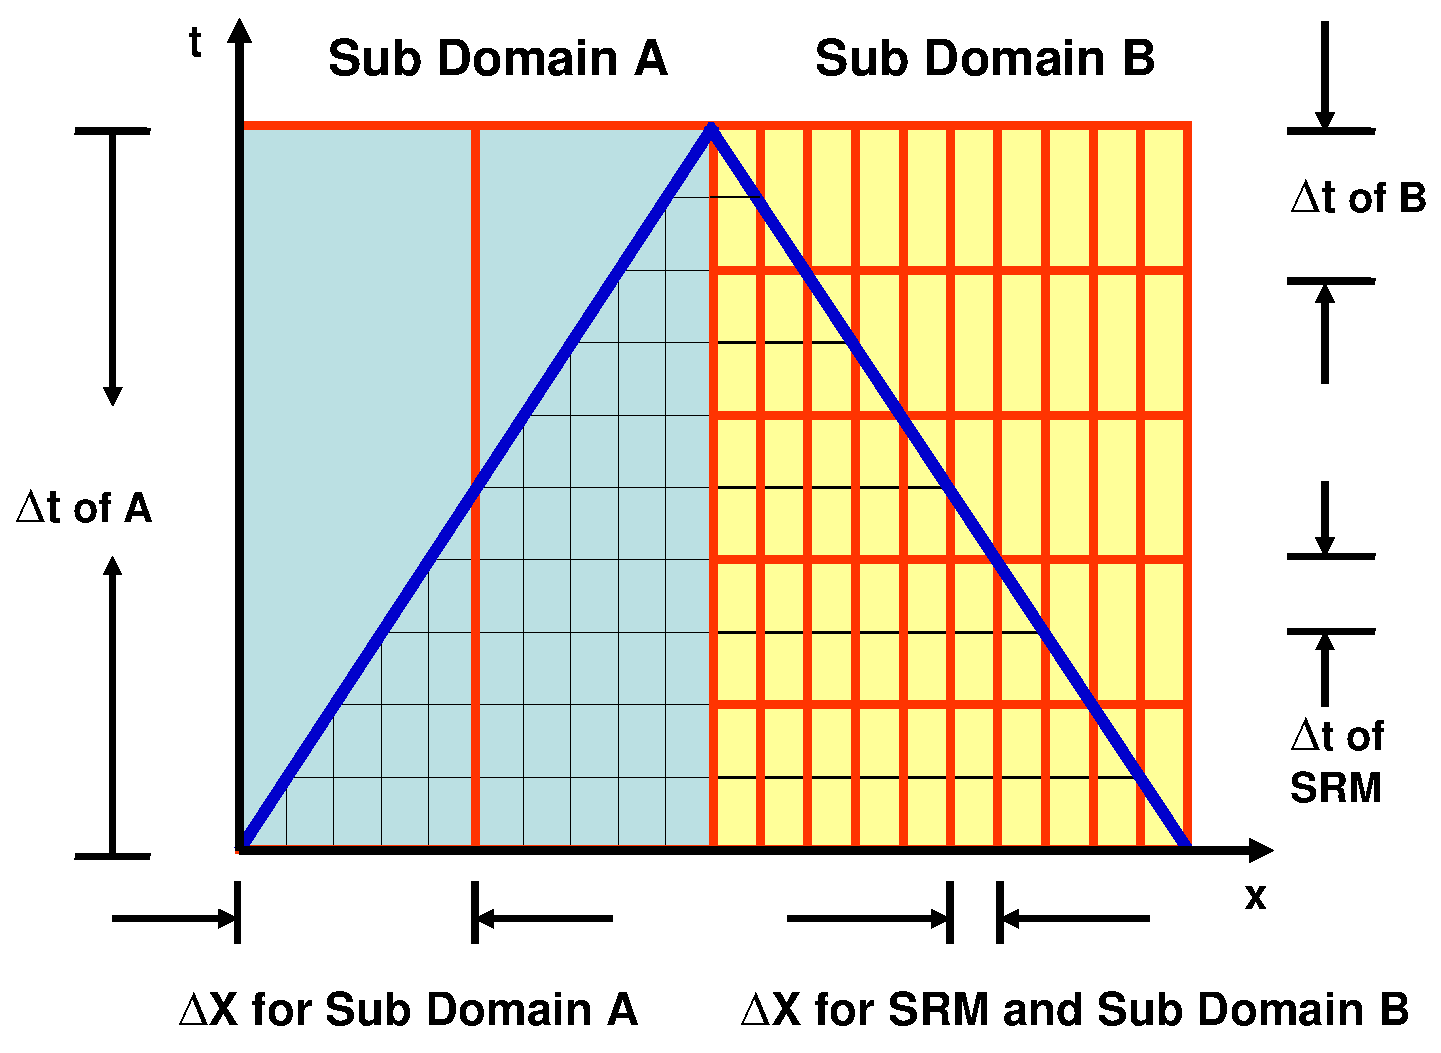
\includegraphics[width=4in]{../figures/SRM/domain.pdf}
    \caption{SRM domain decomposition concept}
    \label{fig:SRM-DDM}
  \end{center}
\end{figure}

\cp

\subsection{Combined Gravity Current and Solitary Wave Test}

In the numerical test, an initially still water profile is released from the left-hand-side region of a two-dimensional closed tank to generate a solitary wave \cite{Laitone1960}, while a finite volume of denser fluid is released from the right-hand-side region to generate gravity currents.
The tank is $1.2 (m)$ long with vertical walls at both ends. The bottom slope is zero. The initial still water profile \cite{The1994, Yue2003} is specified as
\be
\eta = h + A/ \cosh^2 (\f{x}{2} \sqrt{3A})
\ee
where $h=0.115 (m)$ and $A=0.18 (m)$. The density of the finite volume to be released is set to $1200 (kg/cm^3)$ and the ambient fluid has the density of $1200 (kg/cm^3)$.
In the SRM domain decomposition method, the whole computational domain is decomposed into two subdomains. The interface between the two subdomains is explicitly computed with the SRM method. The grid resolution is tested with $\Delta x = 0.01 (m)$ and $\Delta z = 0.01 (m)$. The time step is $\Delta t = 0.01 (sec)$ for subdomains and $\Delta t = 0.00005 (sec)$ for the interface. The under-relaxation parameter $\beta=1$ and the penalty parameter $\epsilon=200$. The viscosity is tested with $10^{-2} (m^2/s)$.
The computation results with the SRM domain decomposition method is plotted in Figure \ref{fig:Wave-GravityCurrent-SRM-DDM}, this can be qualitatively compared with the results with the flow model of Chapter \ref{chapter:FlowModel} plotted in Figure \ref{fig:Wave-GravityCurrent-Proj}.

% soli = 0.001*Am0/cosh(0.5*0.001*(i-1)*sqrt(3*Am0))**2 + h0

\begin{figure}[h]
\begin{center}
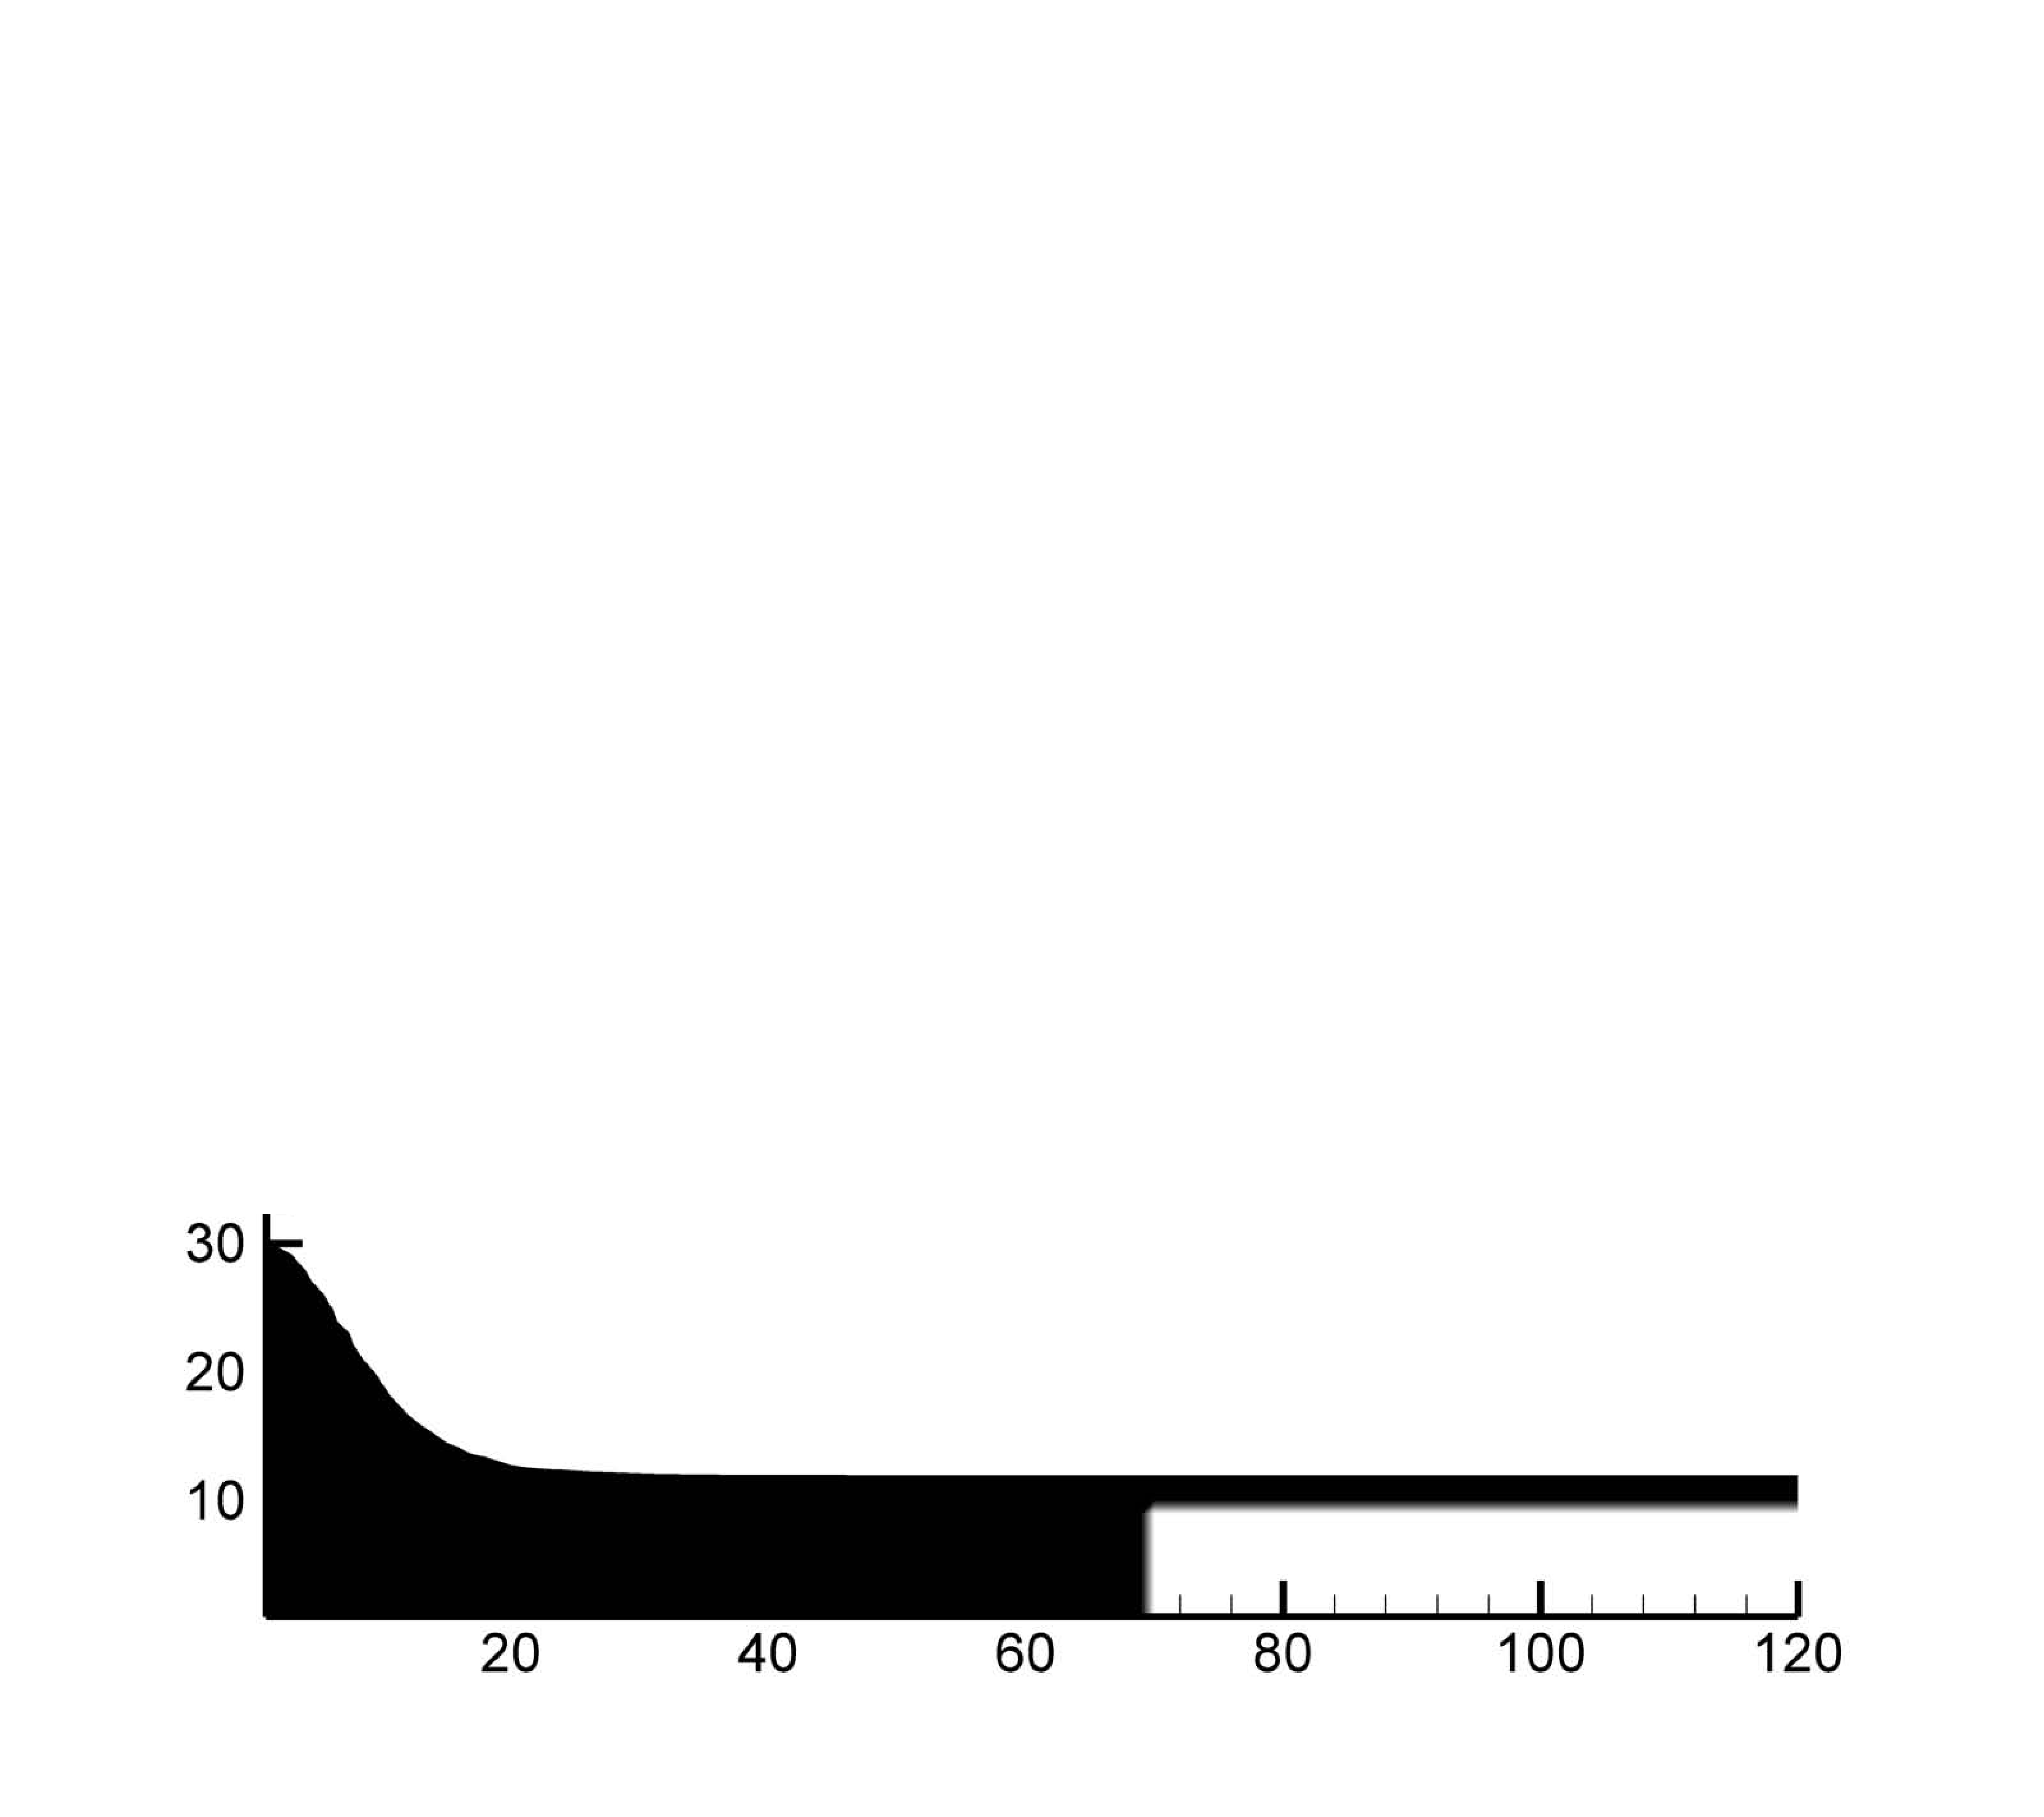
\includegraphics[width=3.5in]{../figures/SRM/SRM-DDM-000.pdf}
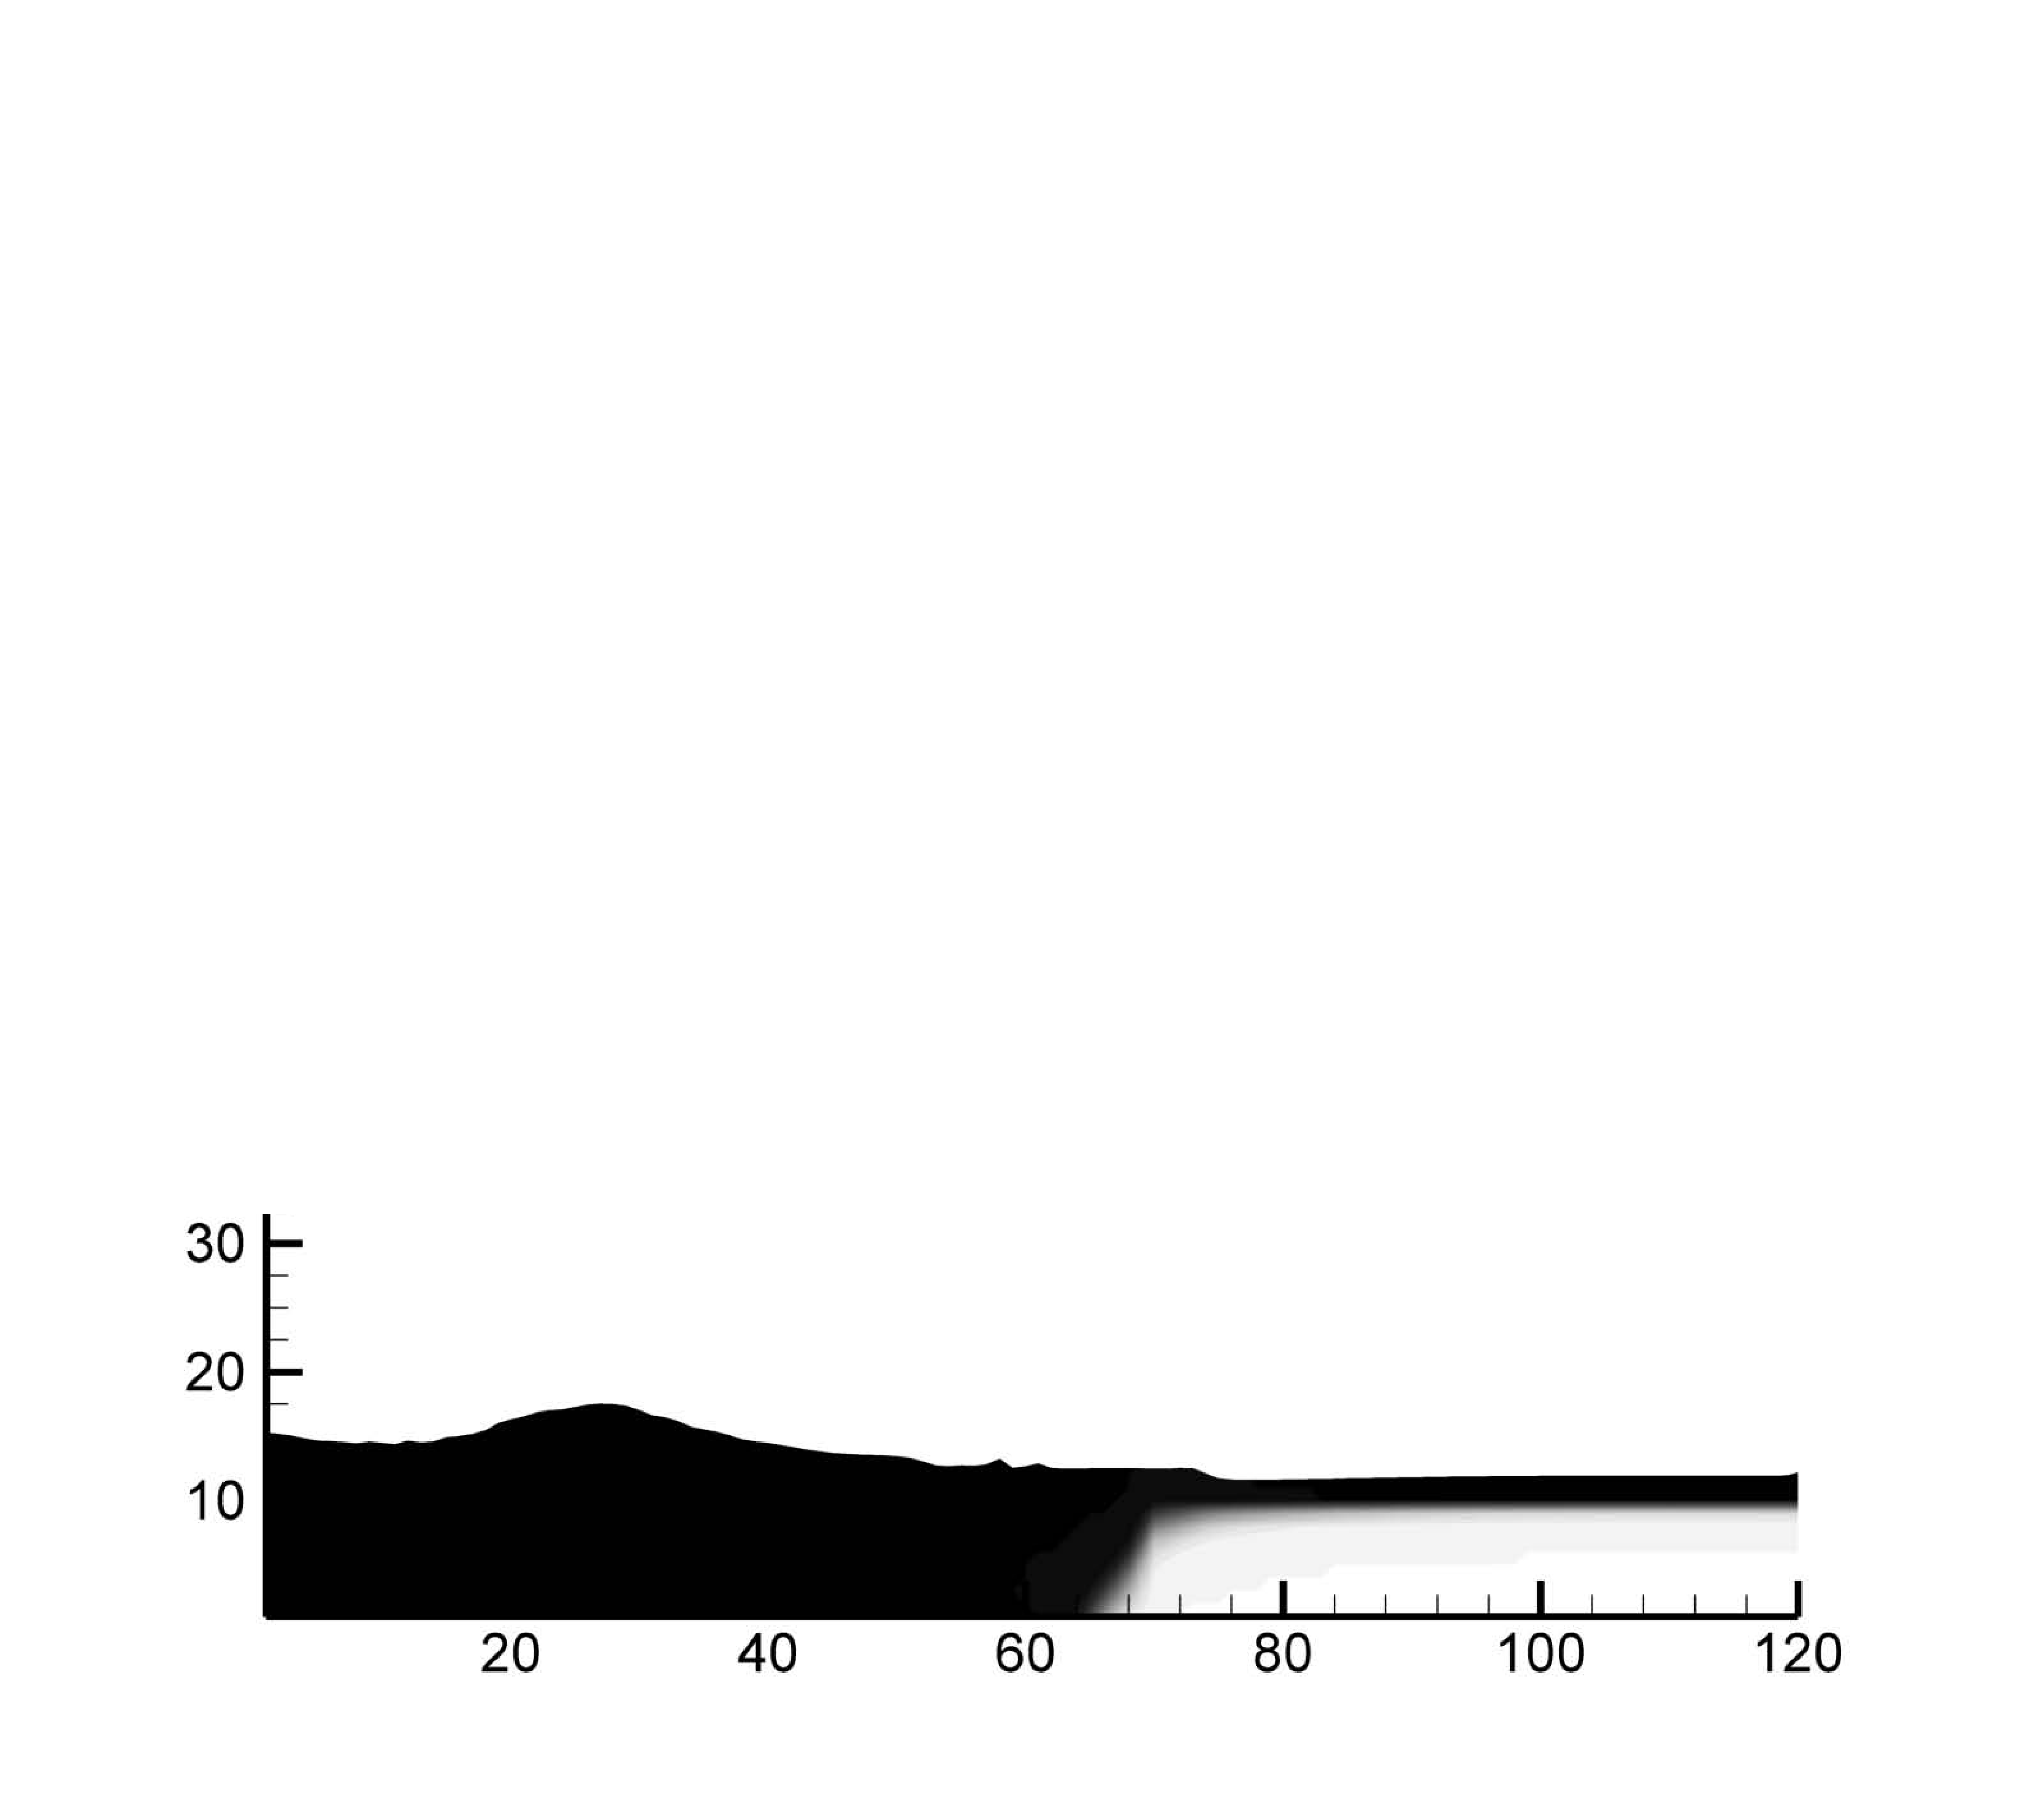
\includegraphics[width=3.5in]{../figures/SRM/SRM-DDM-025.pdf}
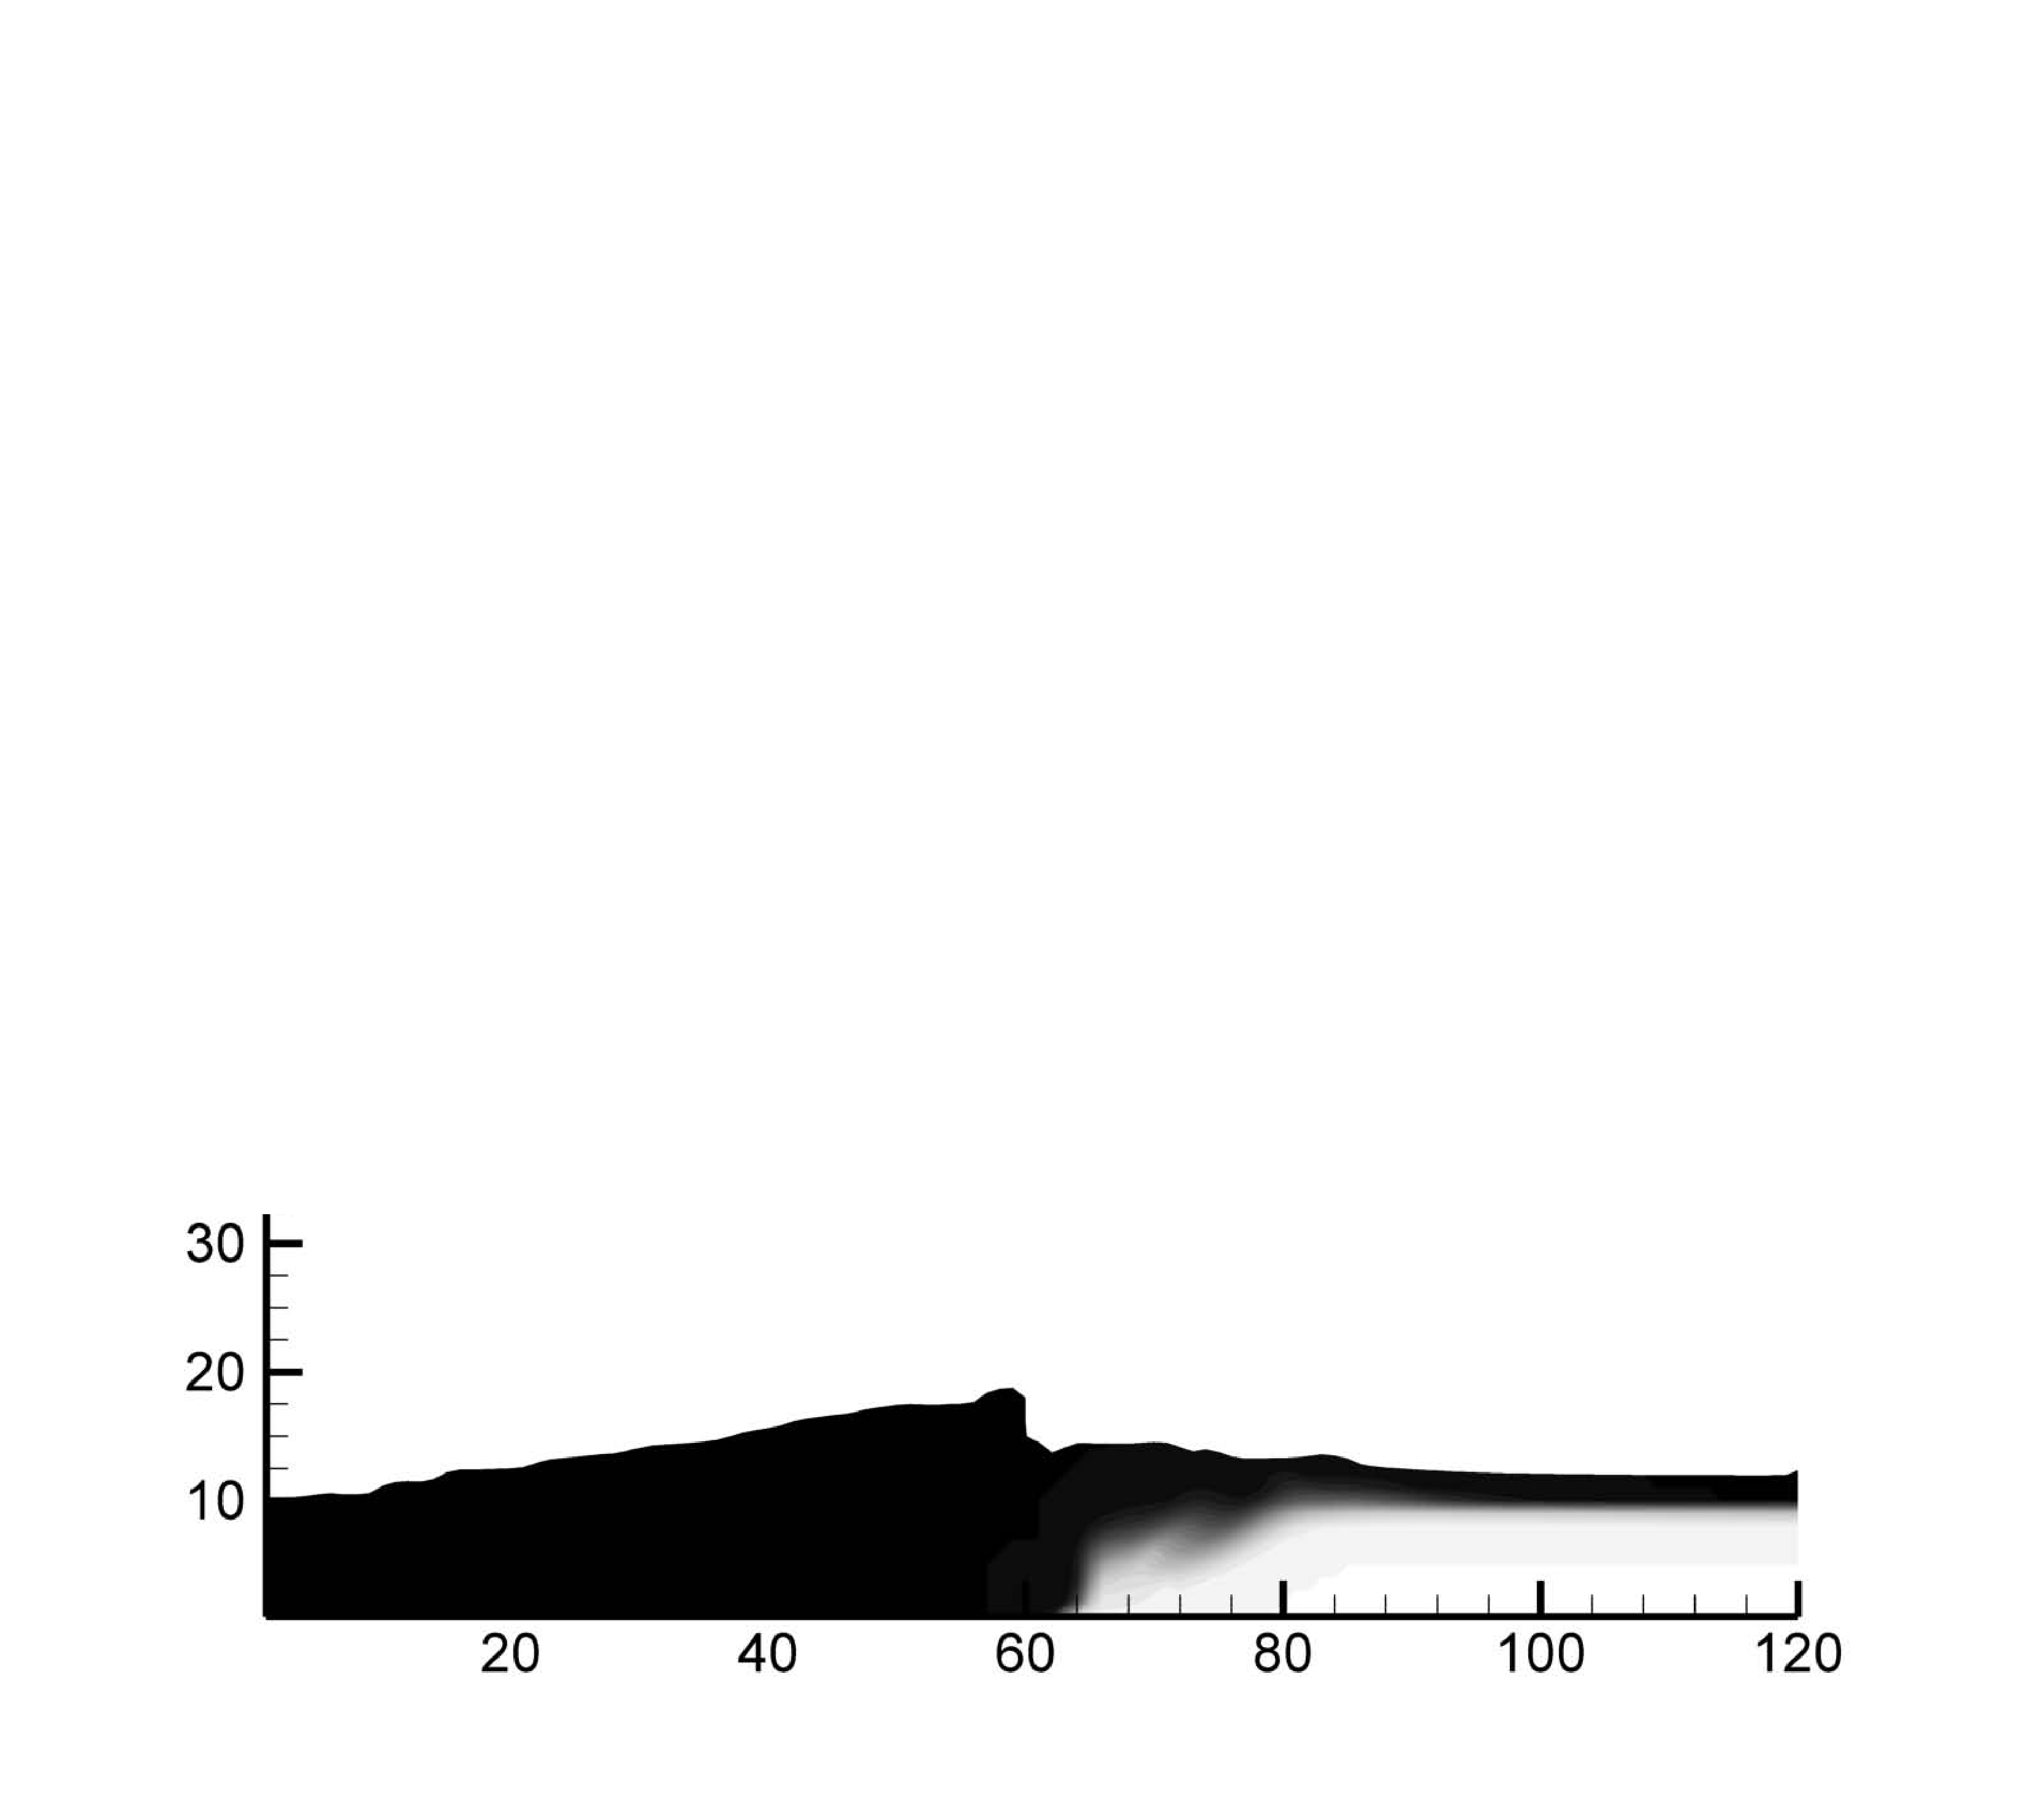
\includegraphics[width=3.5in]{../figures/SRM/SRM-DDM-050.pdf}
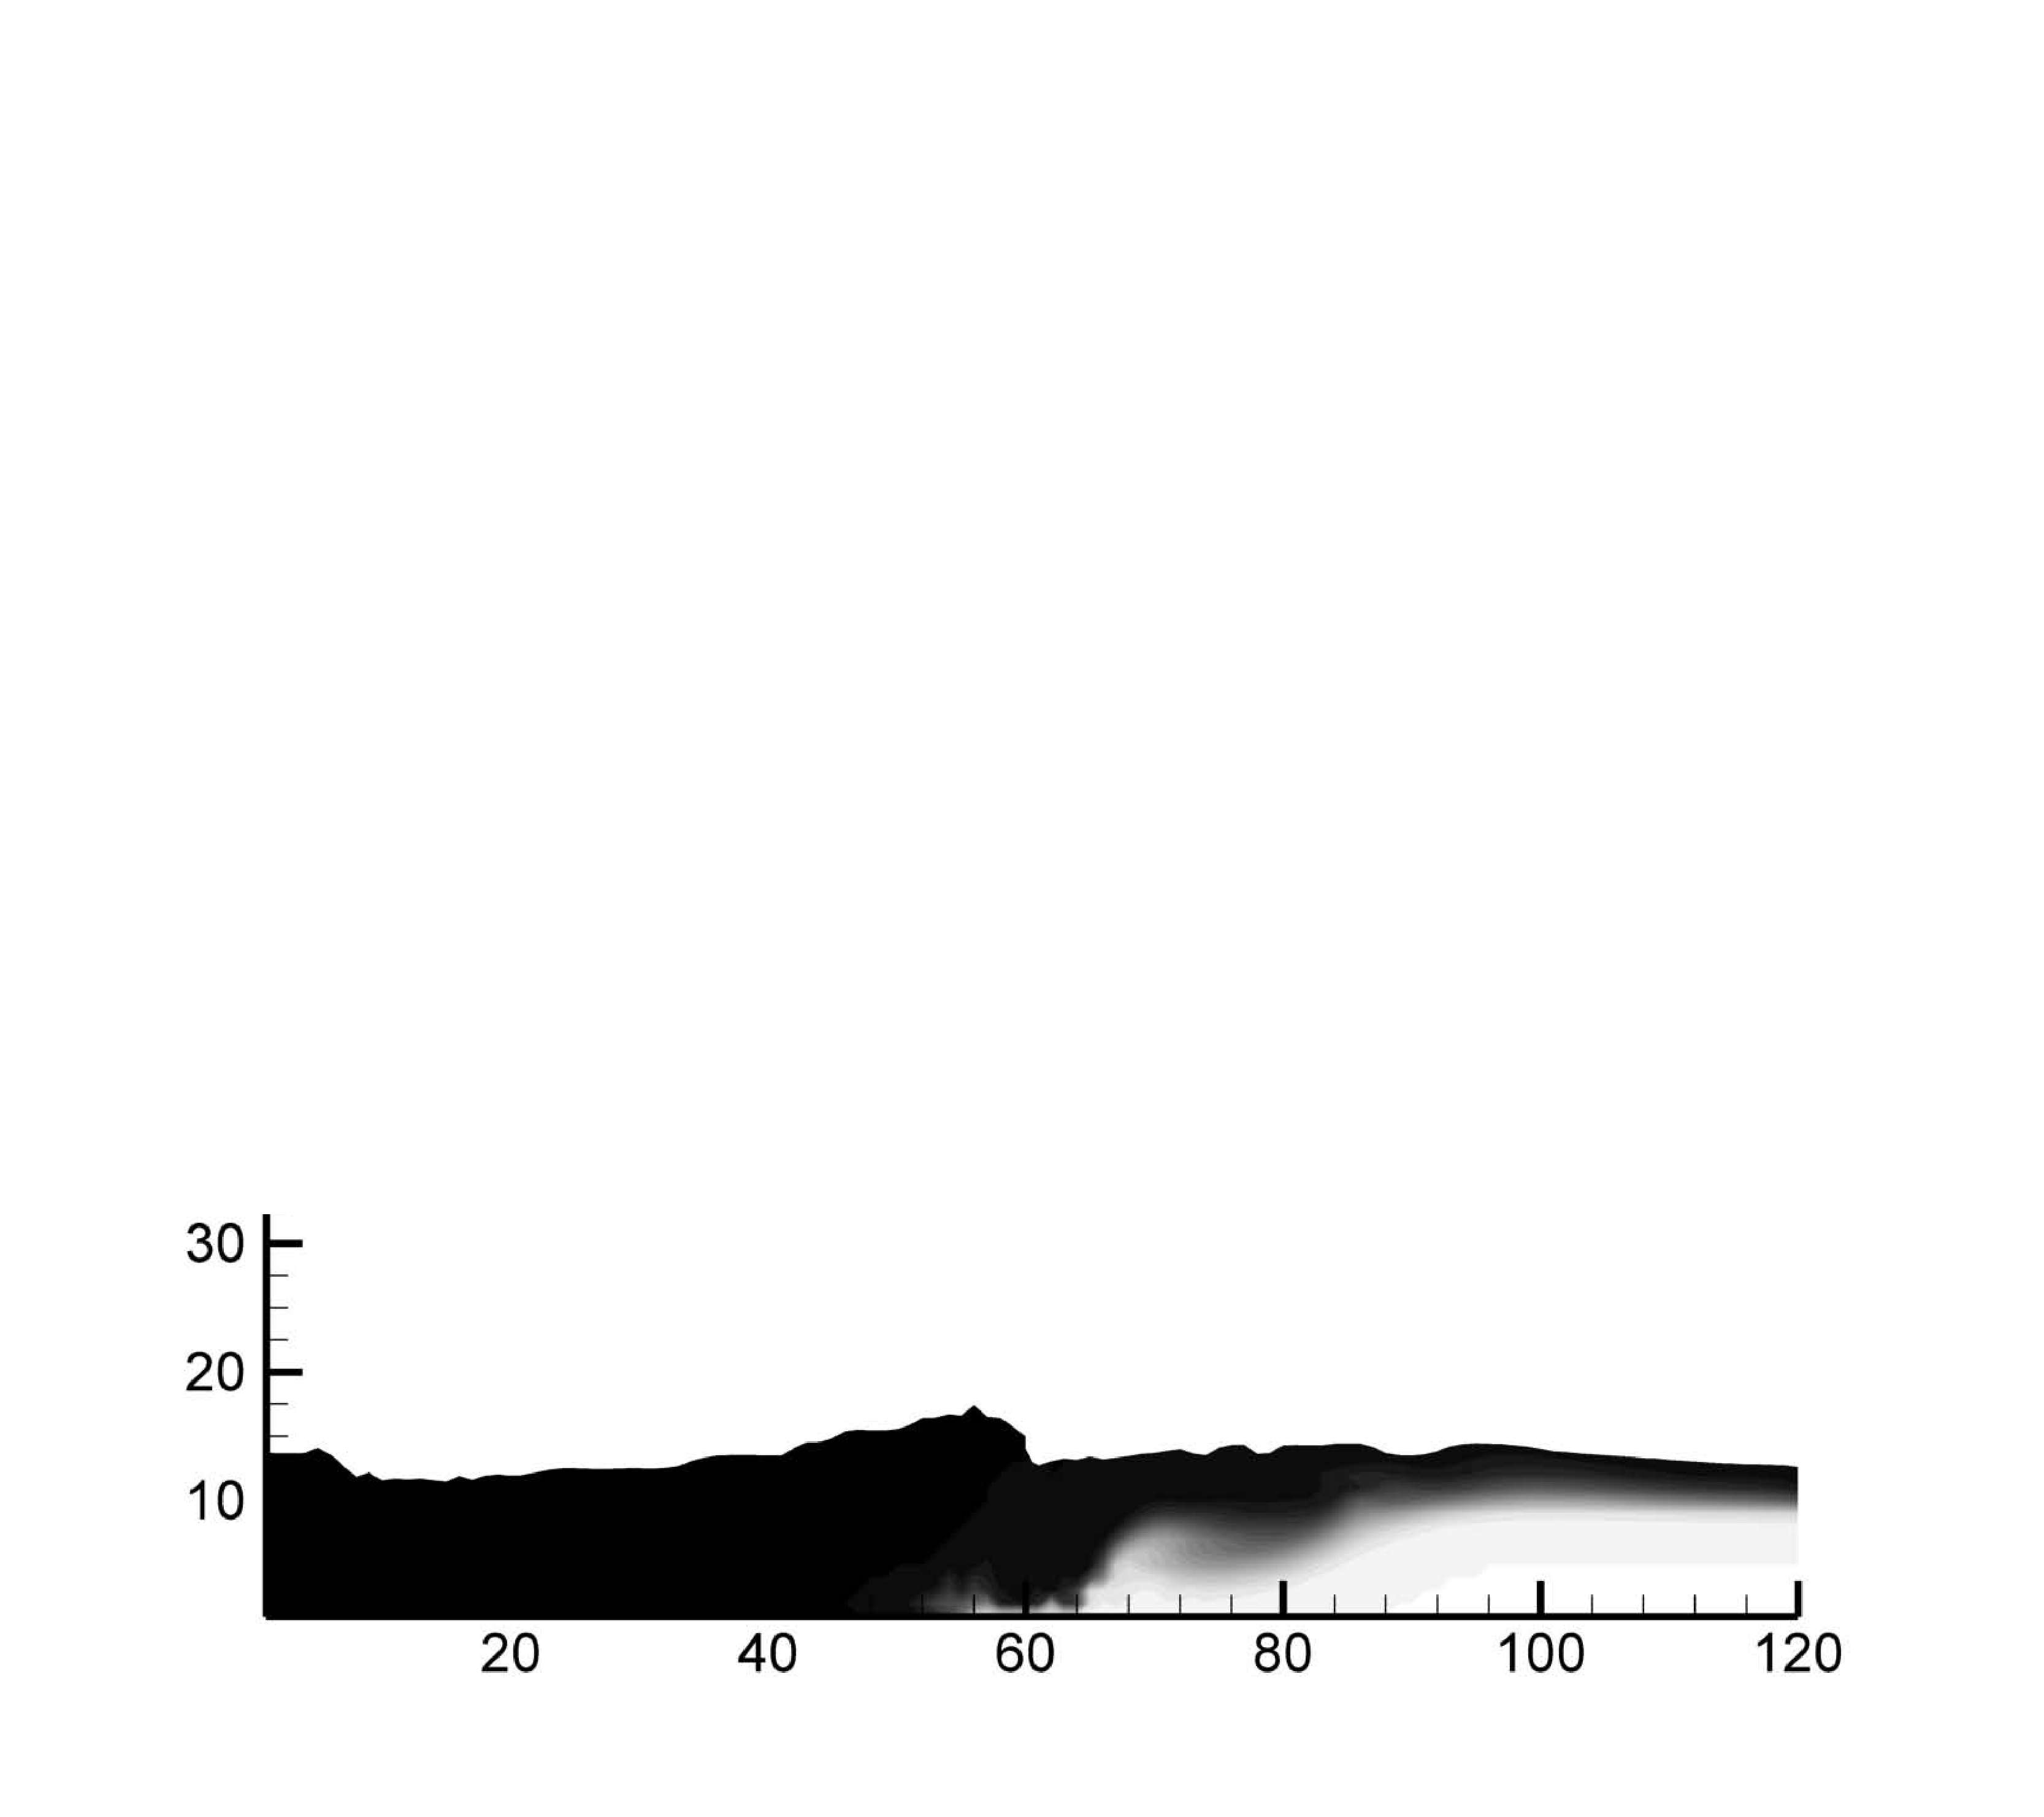
\includegraphics[width=3.5in]{../figures/SRM/SRM-DDM-075.pdf}
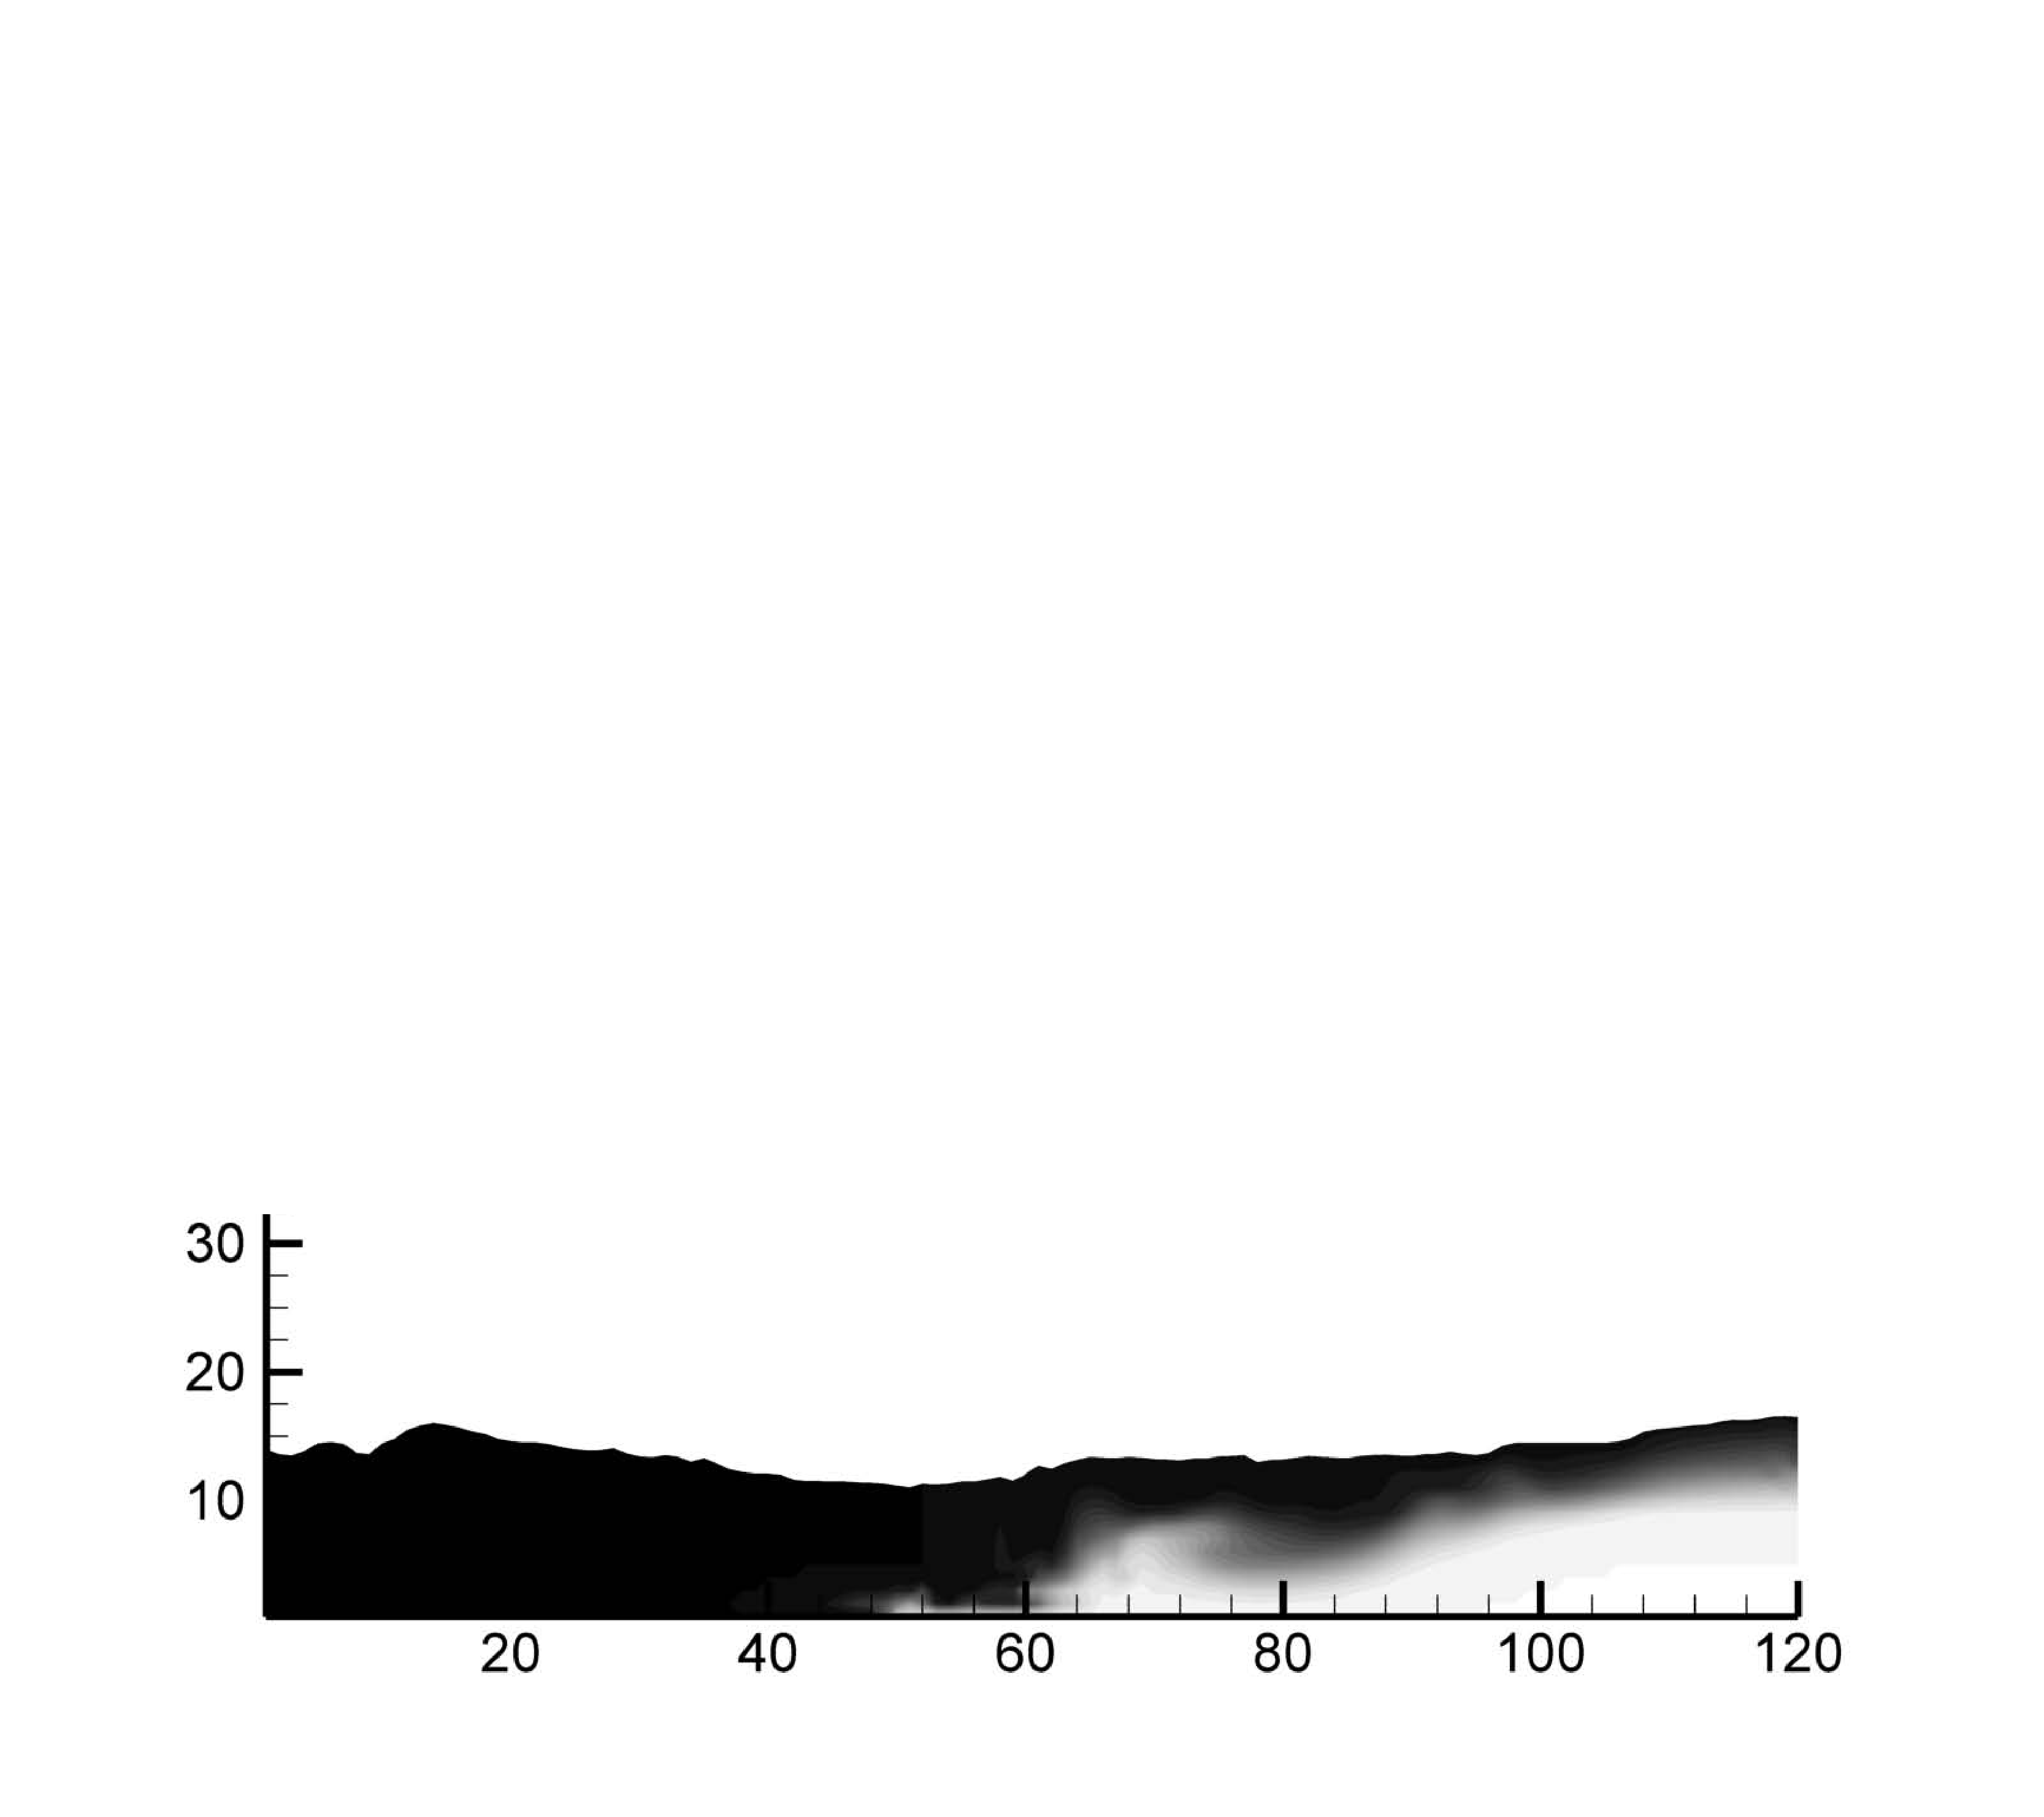
\includegraphics[width=3.5in]{../figures/SRM/SRM-DDM-100.pdf}
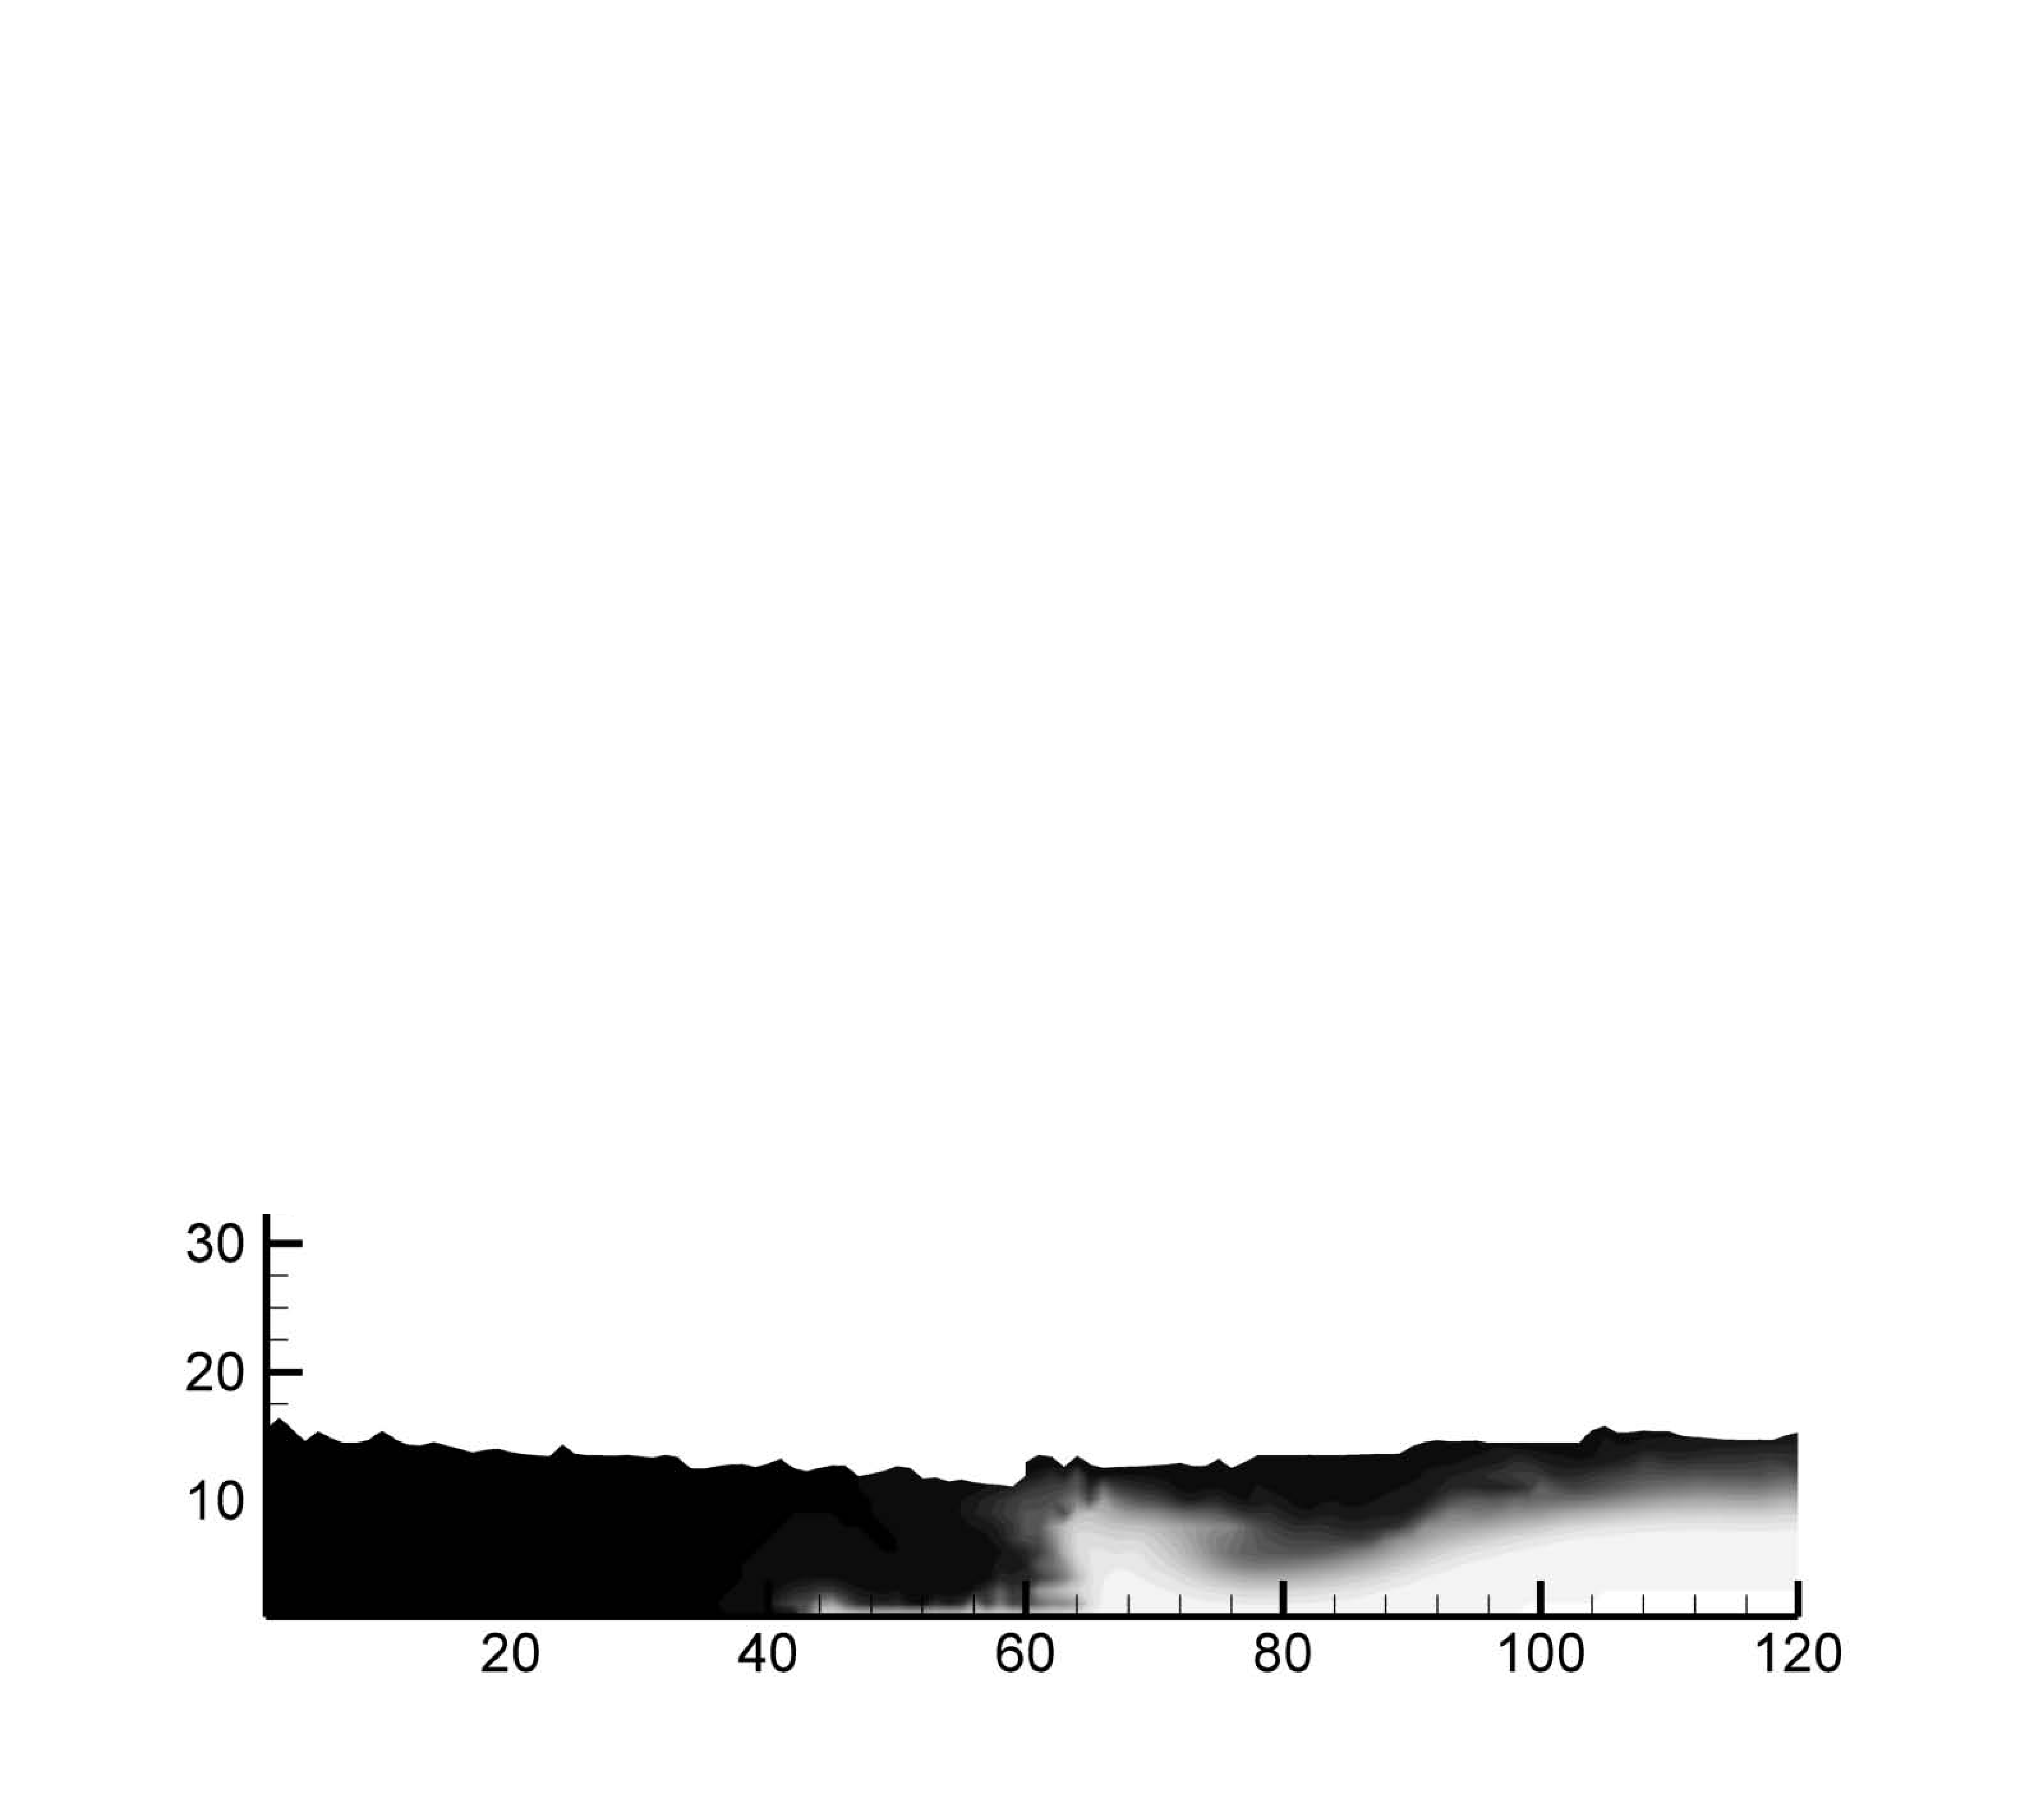
\includegraphics[width=3.5in]{../figures/SRM/SRM-DDM-125.pdf}
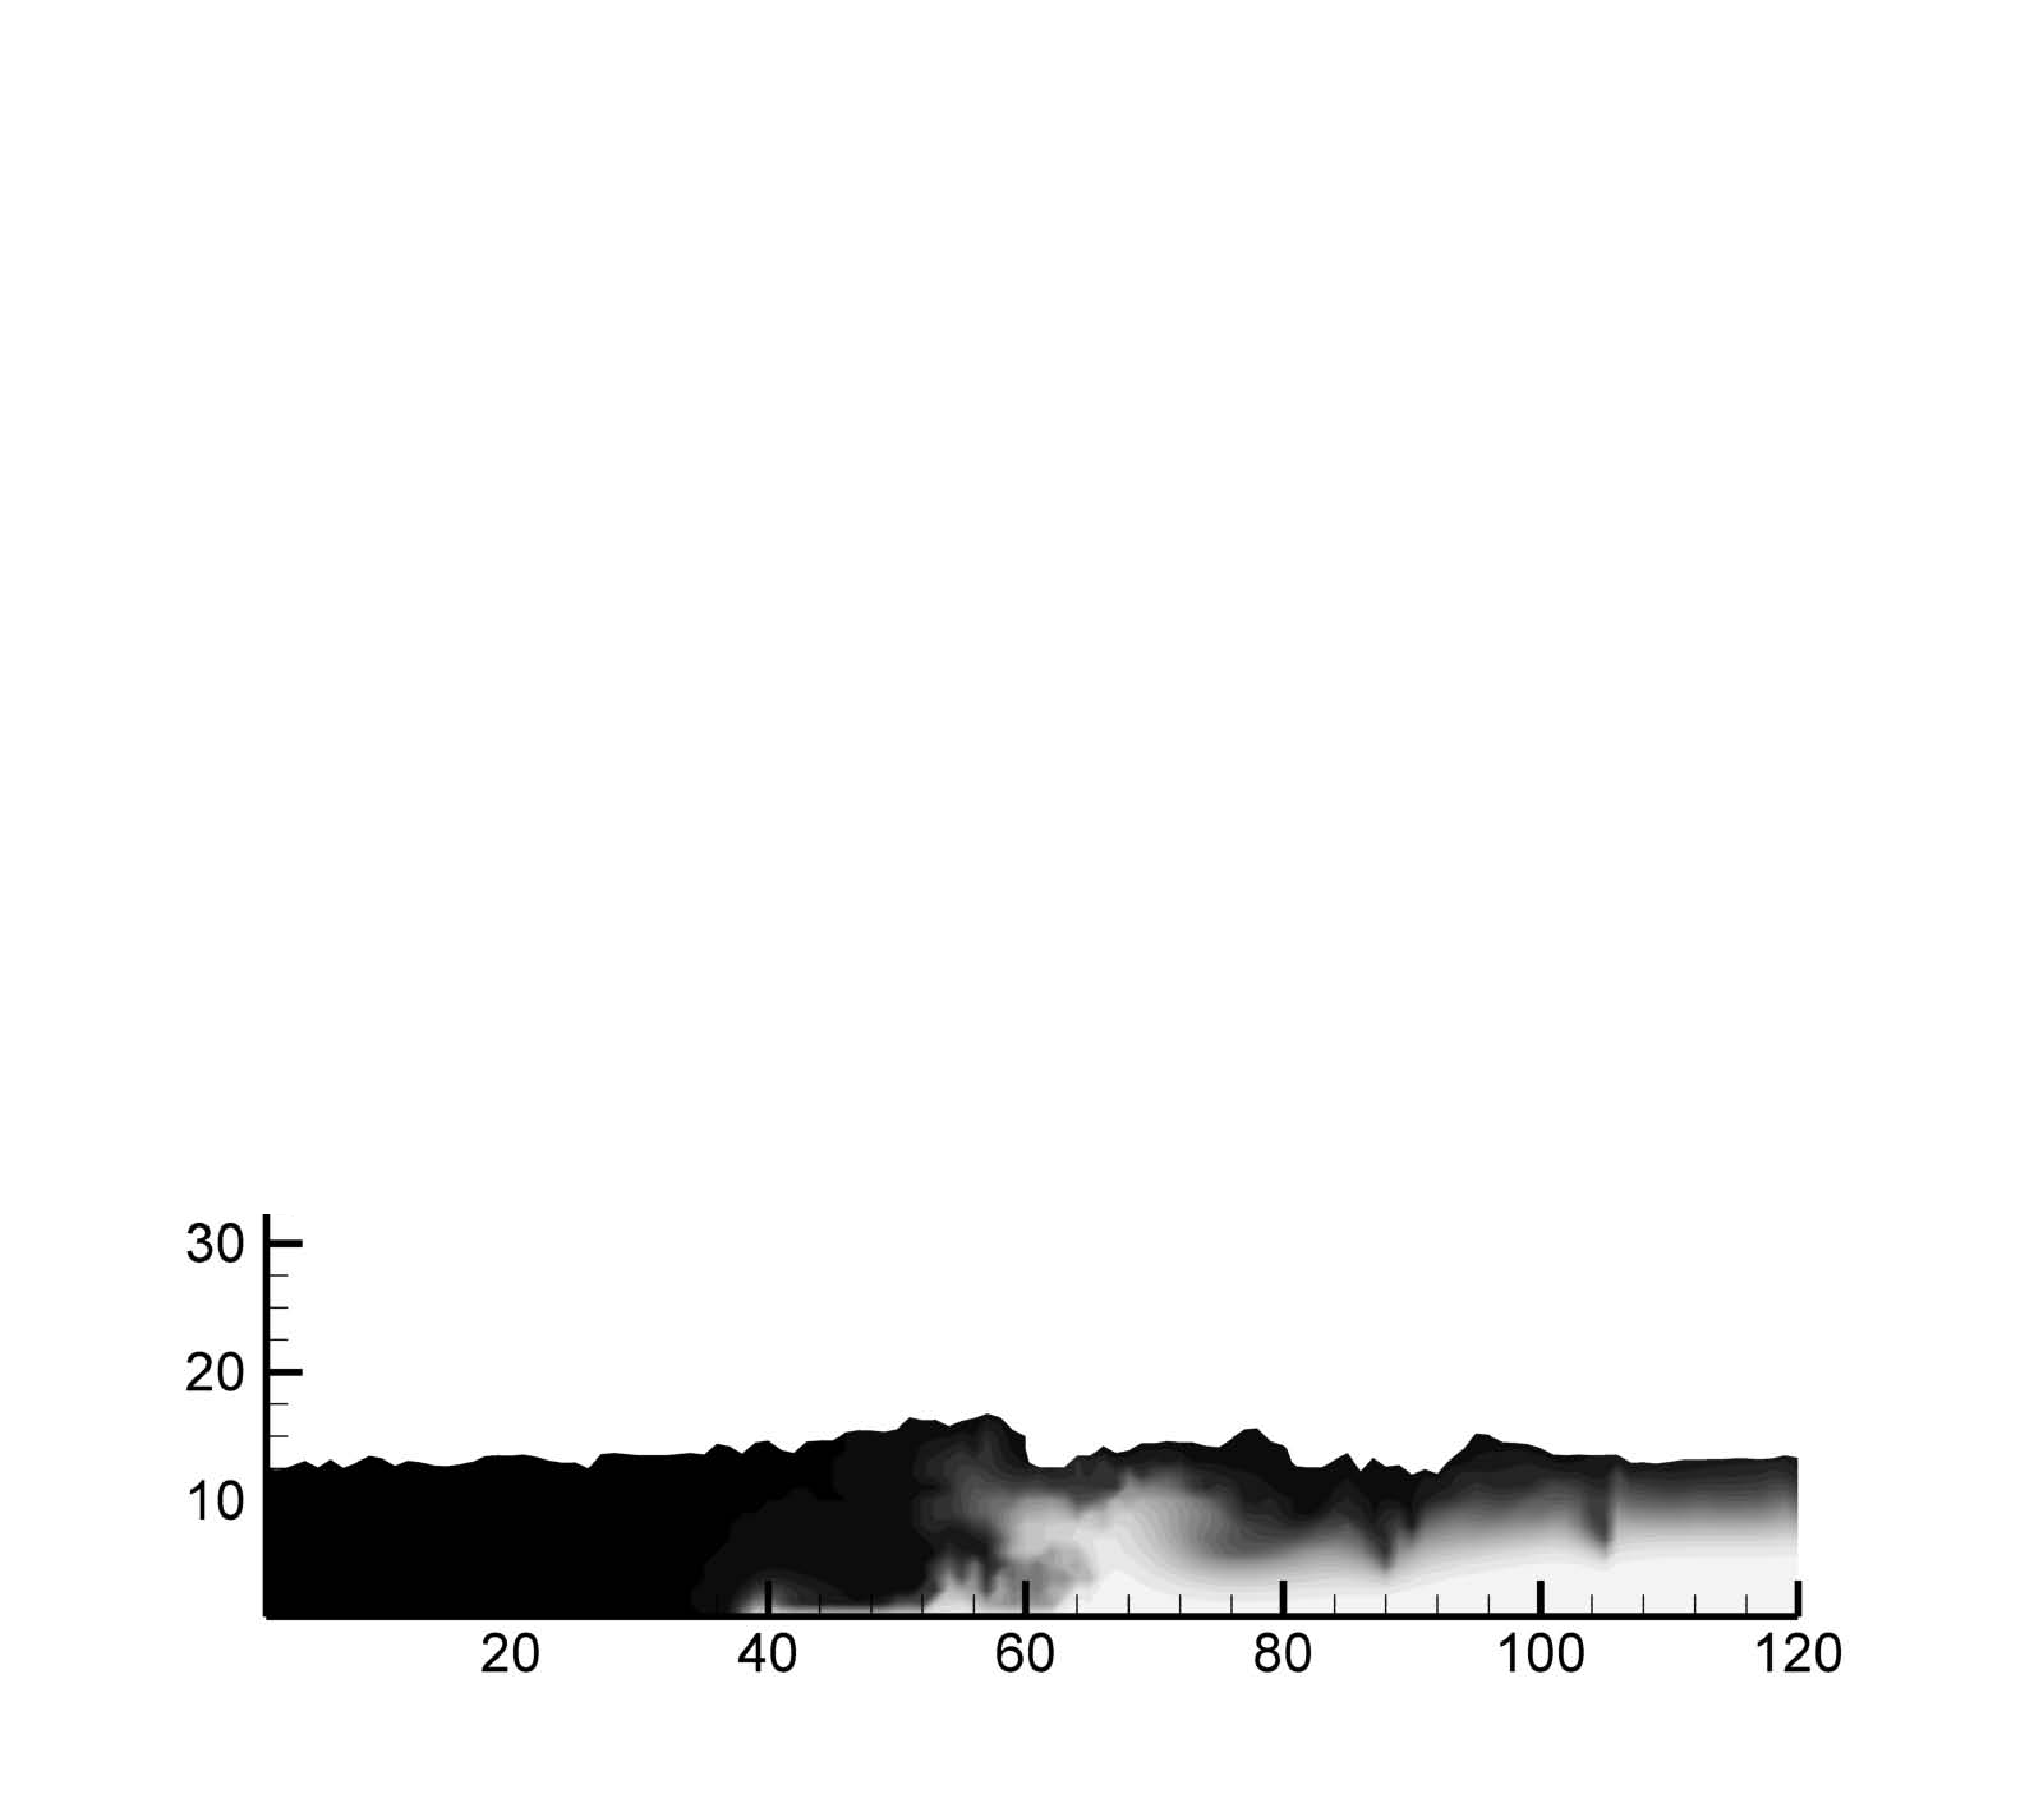
\includegraphics[width=3.5in]{../figures/SRM/SRM-DDM-150.pdf}
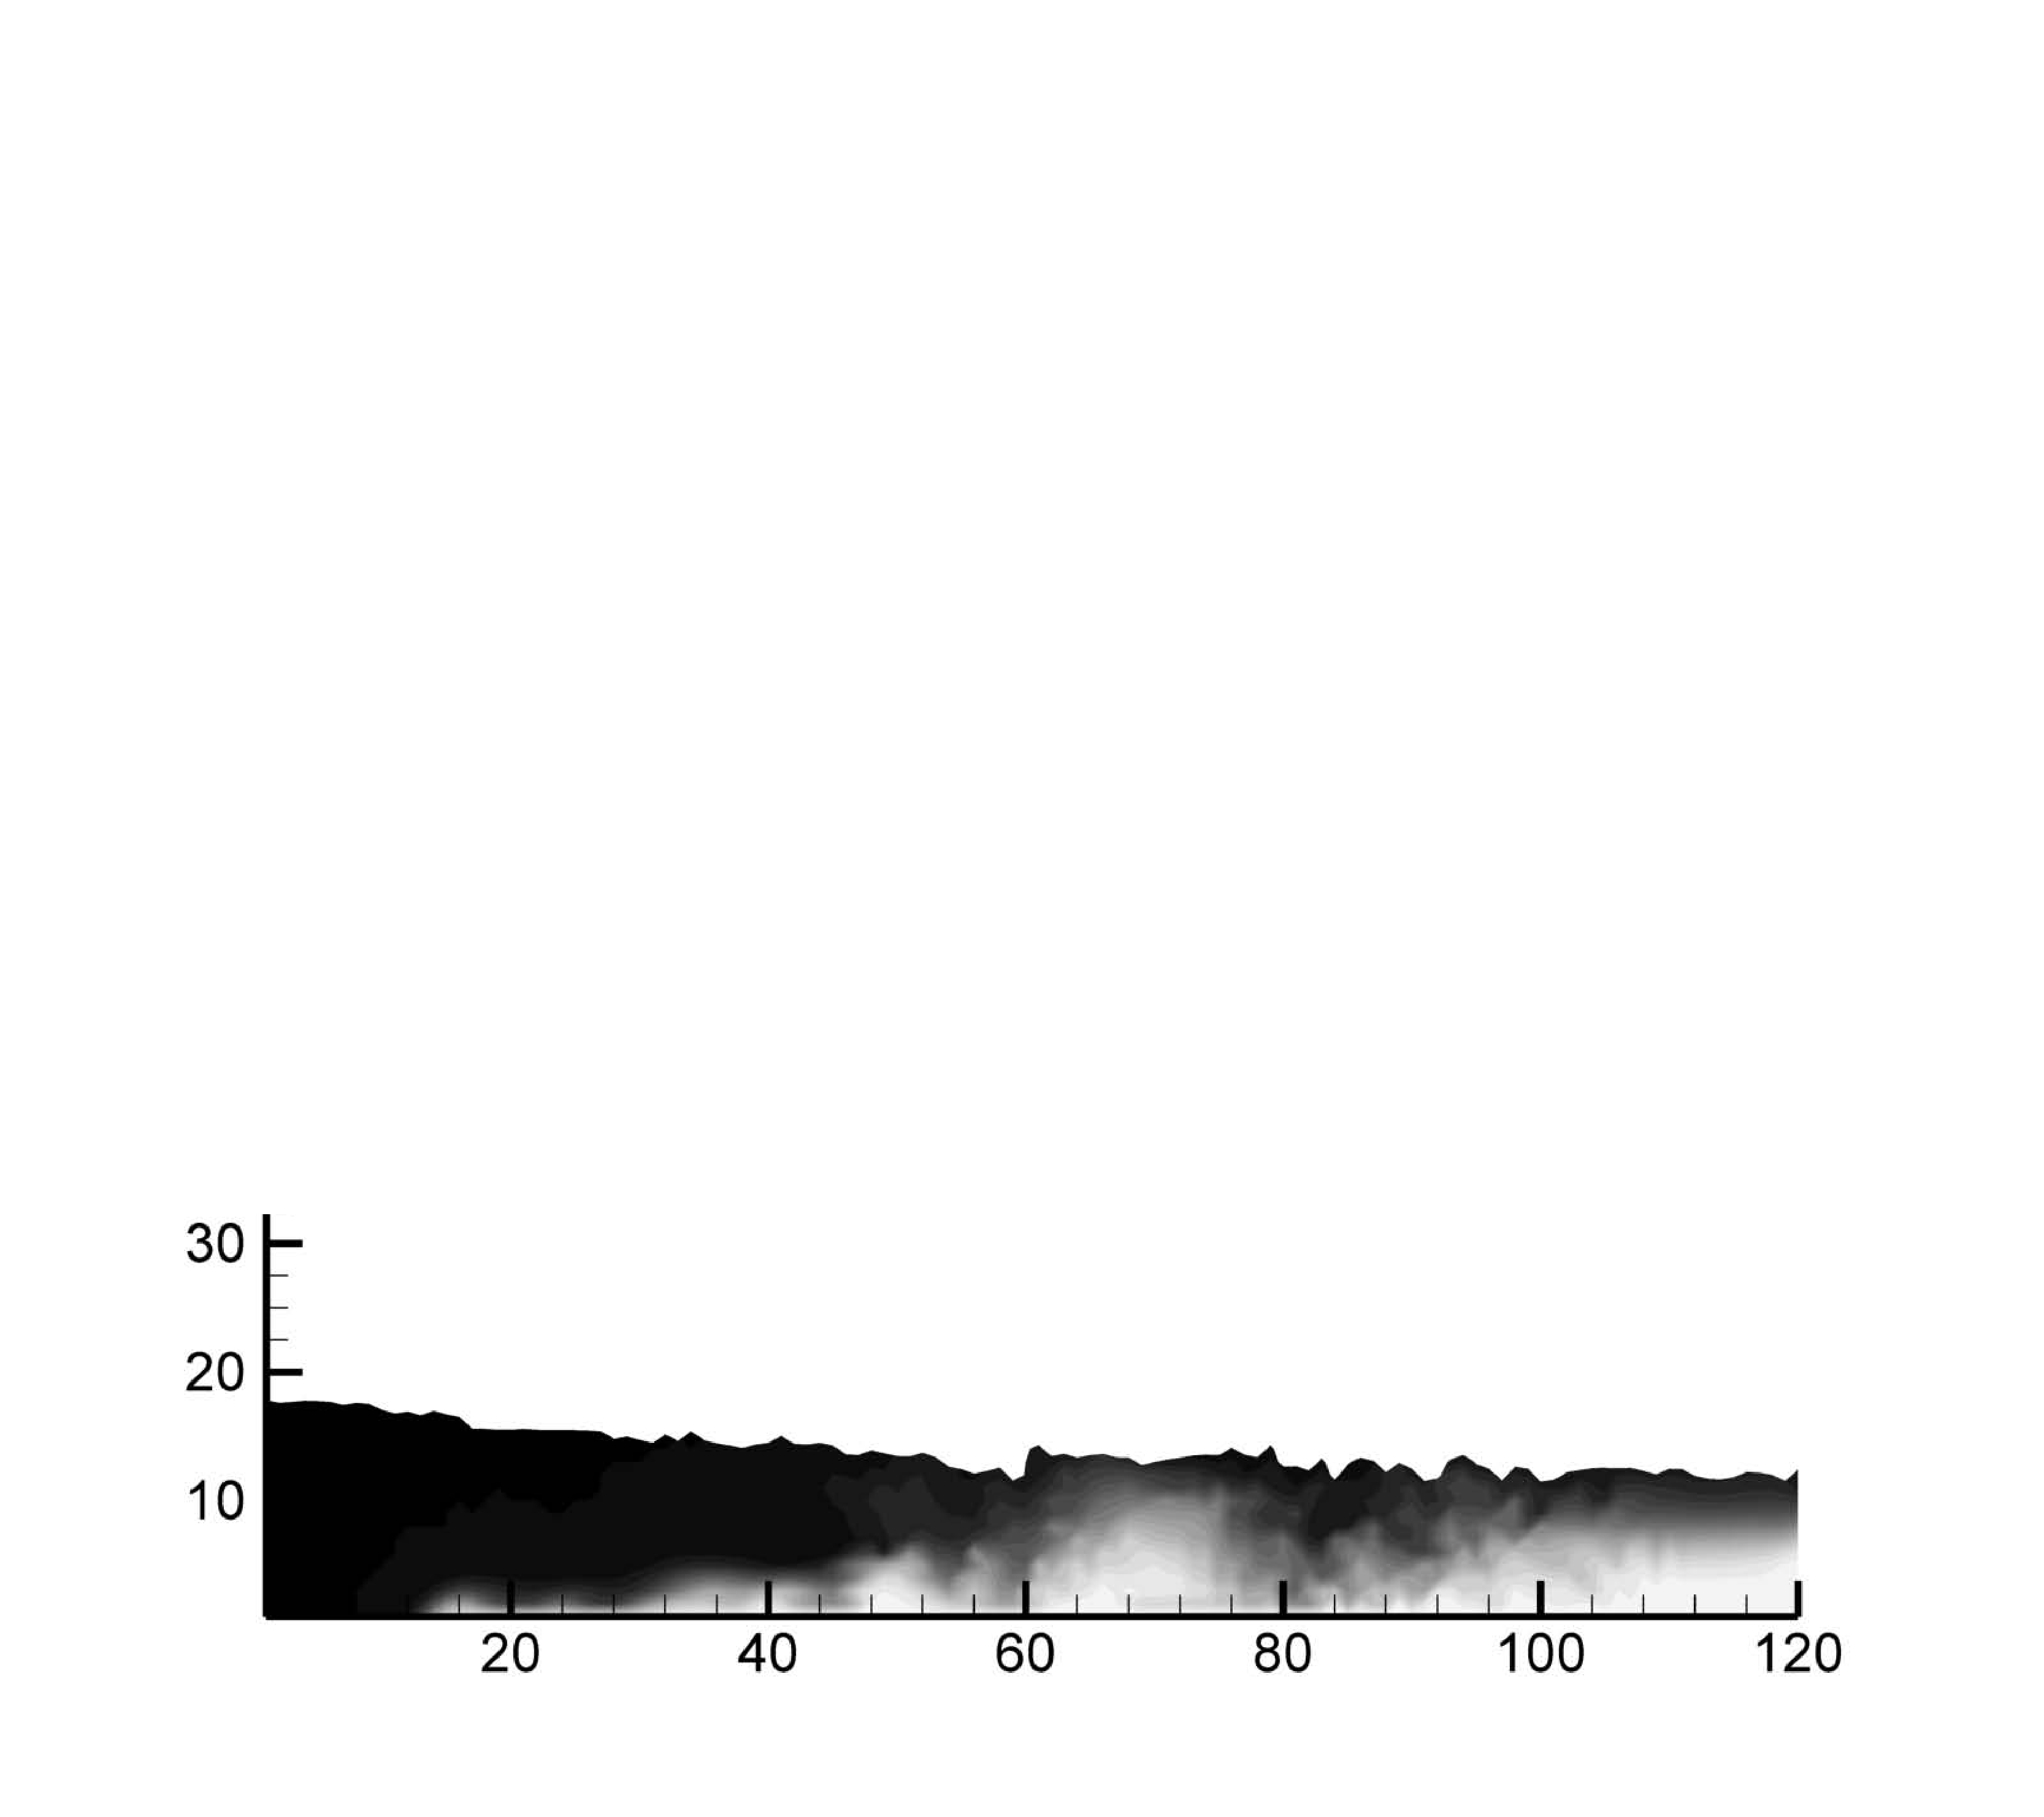
\includegraphics[width=3.5in]{../figures/SRM/SRM-DDM-200.pdf}
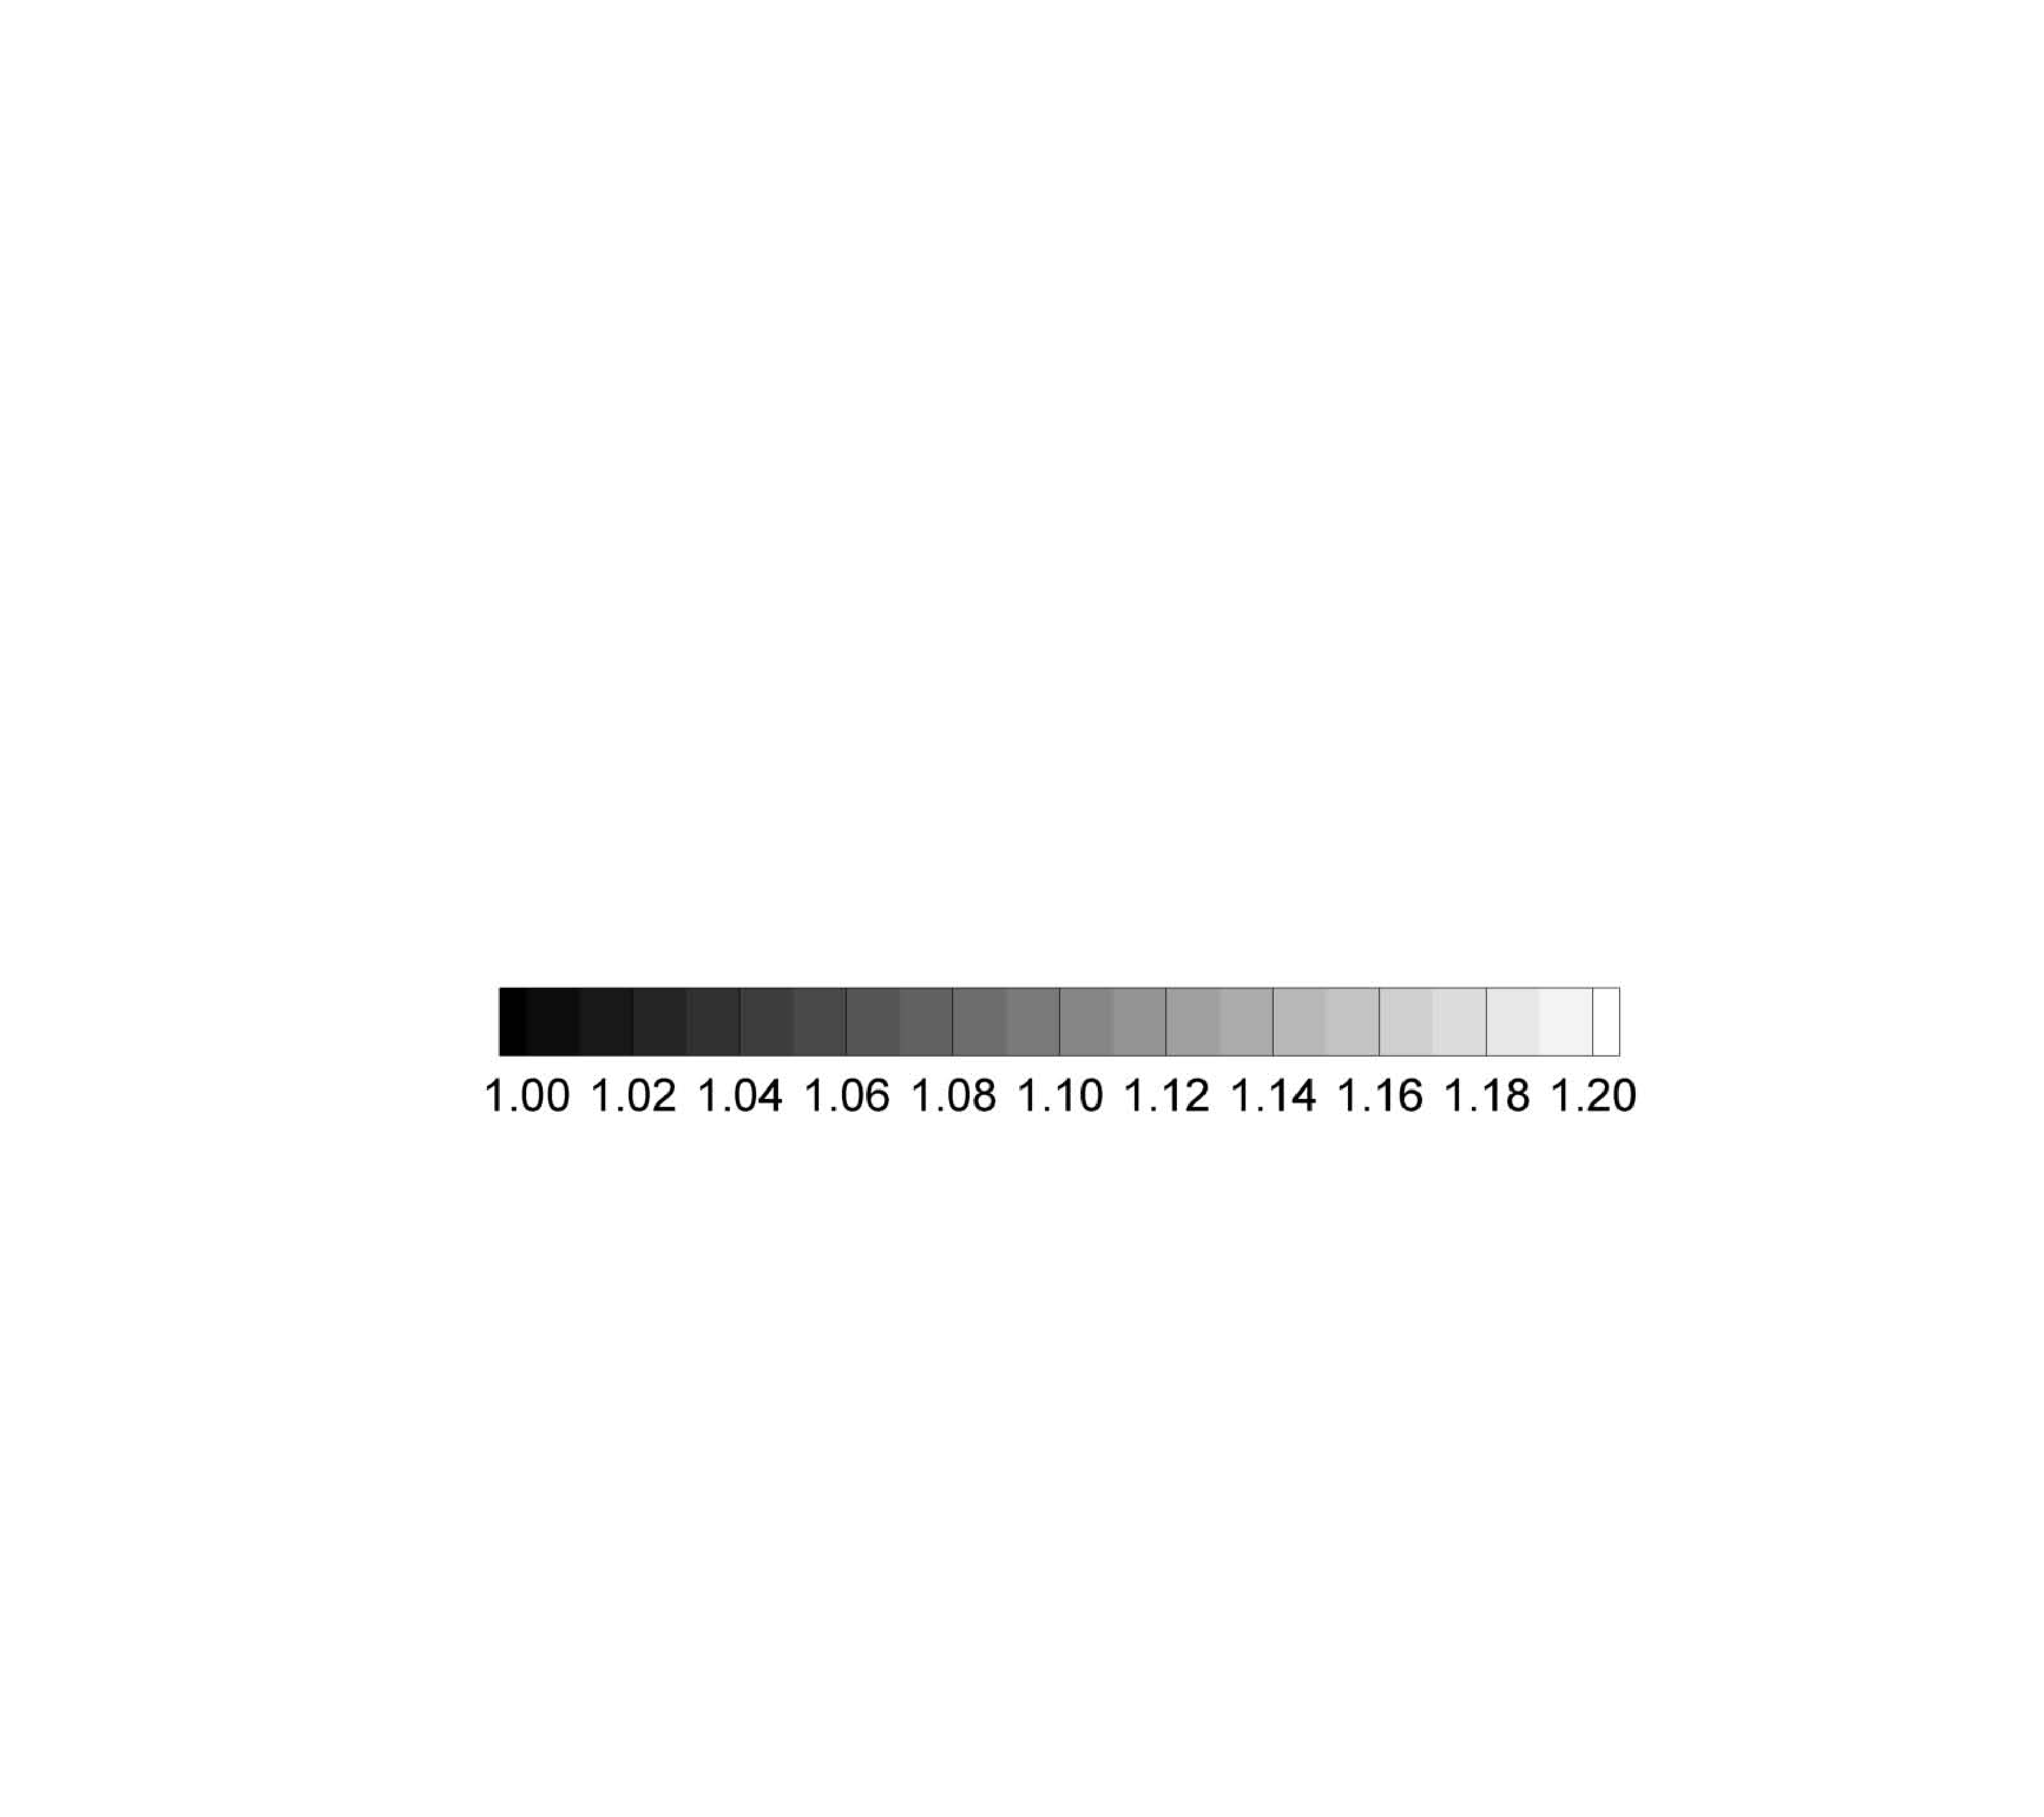
\includegraphics[width=3.0in]{../figures/SRM/contour.pdf}
\end{center}
    \caption{Domain decomposition with sequential regularization method. }
    \label{fig:Wave-GravityCurrent-SRM-DDM}
\end{figure}

\begin{figure}[h]
\begin{center}
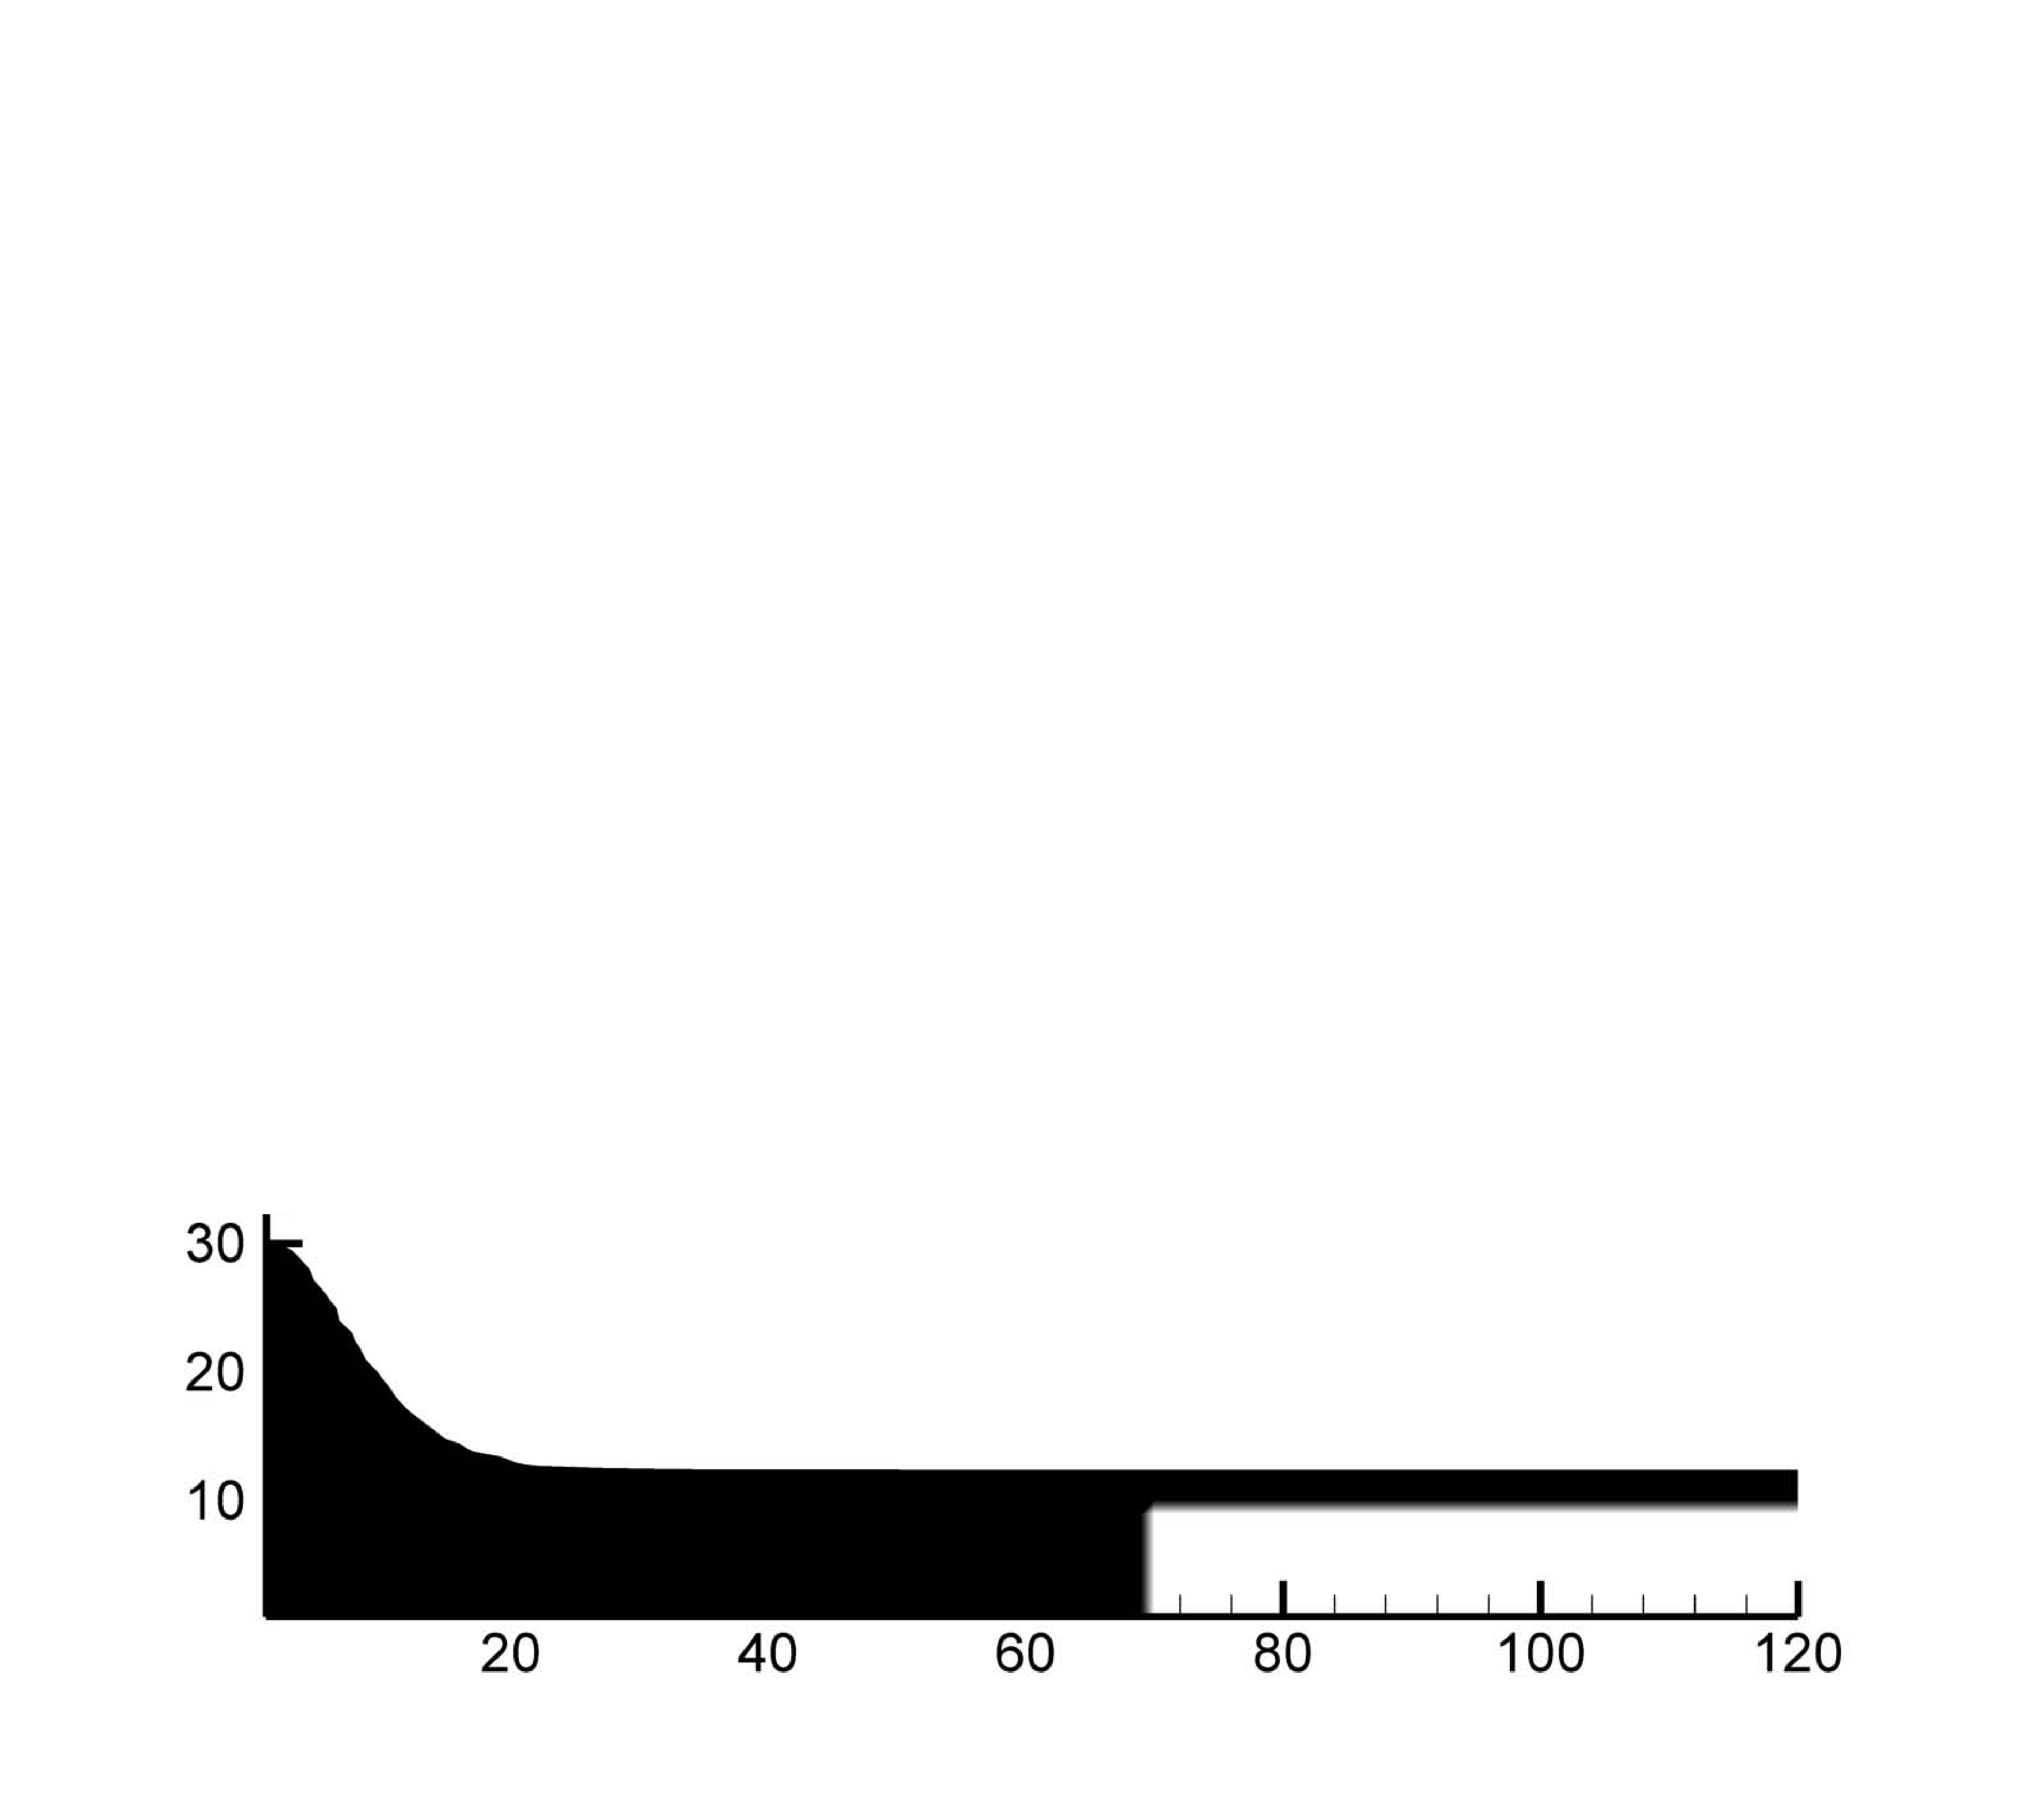
\includegraphics[width=3.5in]{../figures/SRM/000.pdf}
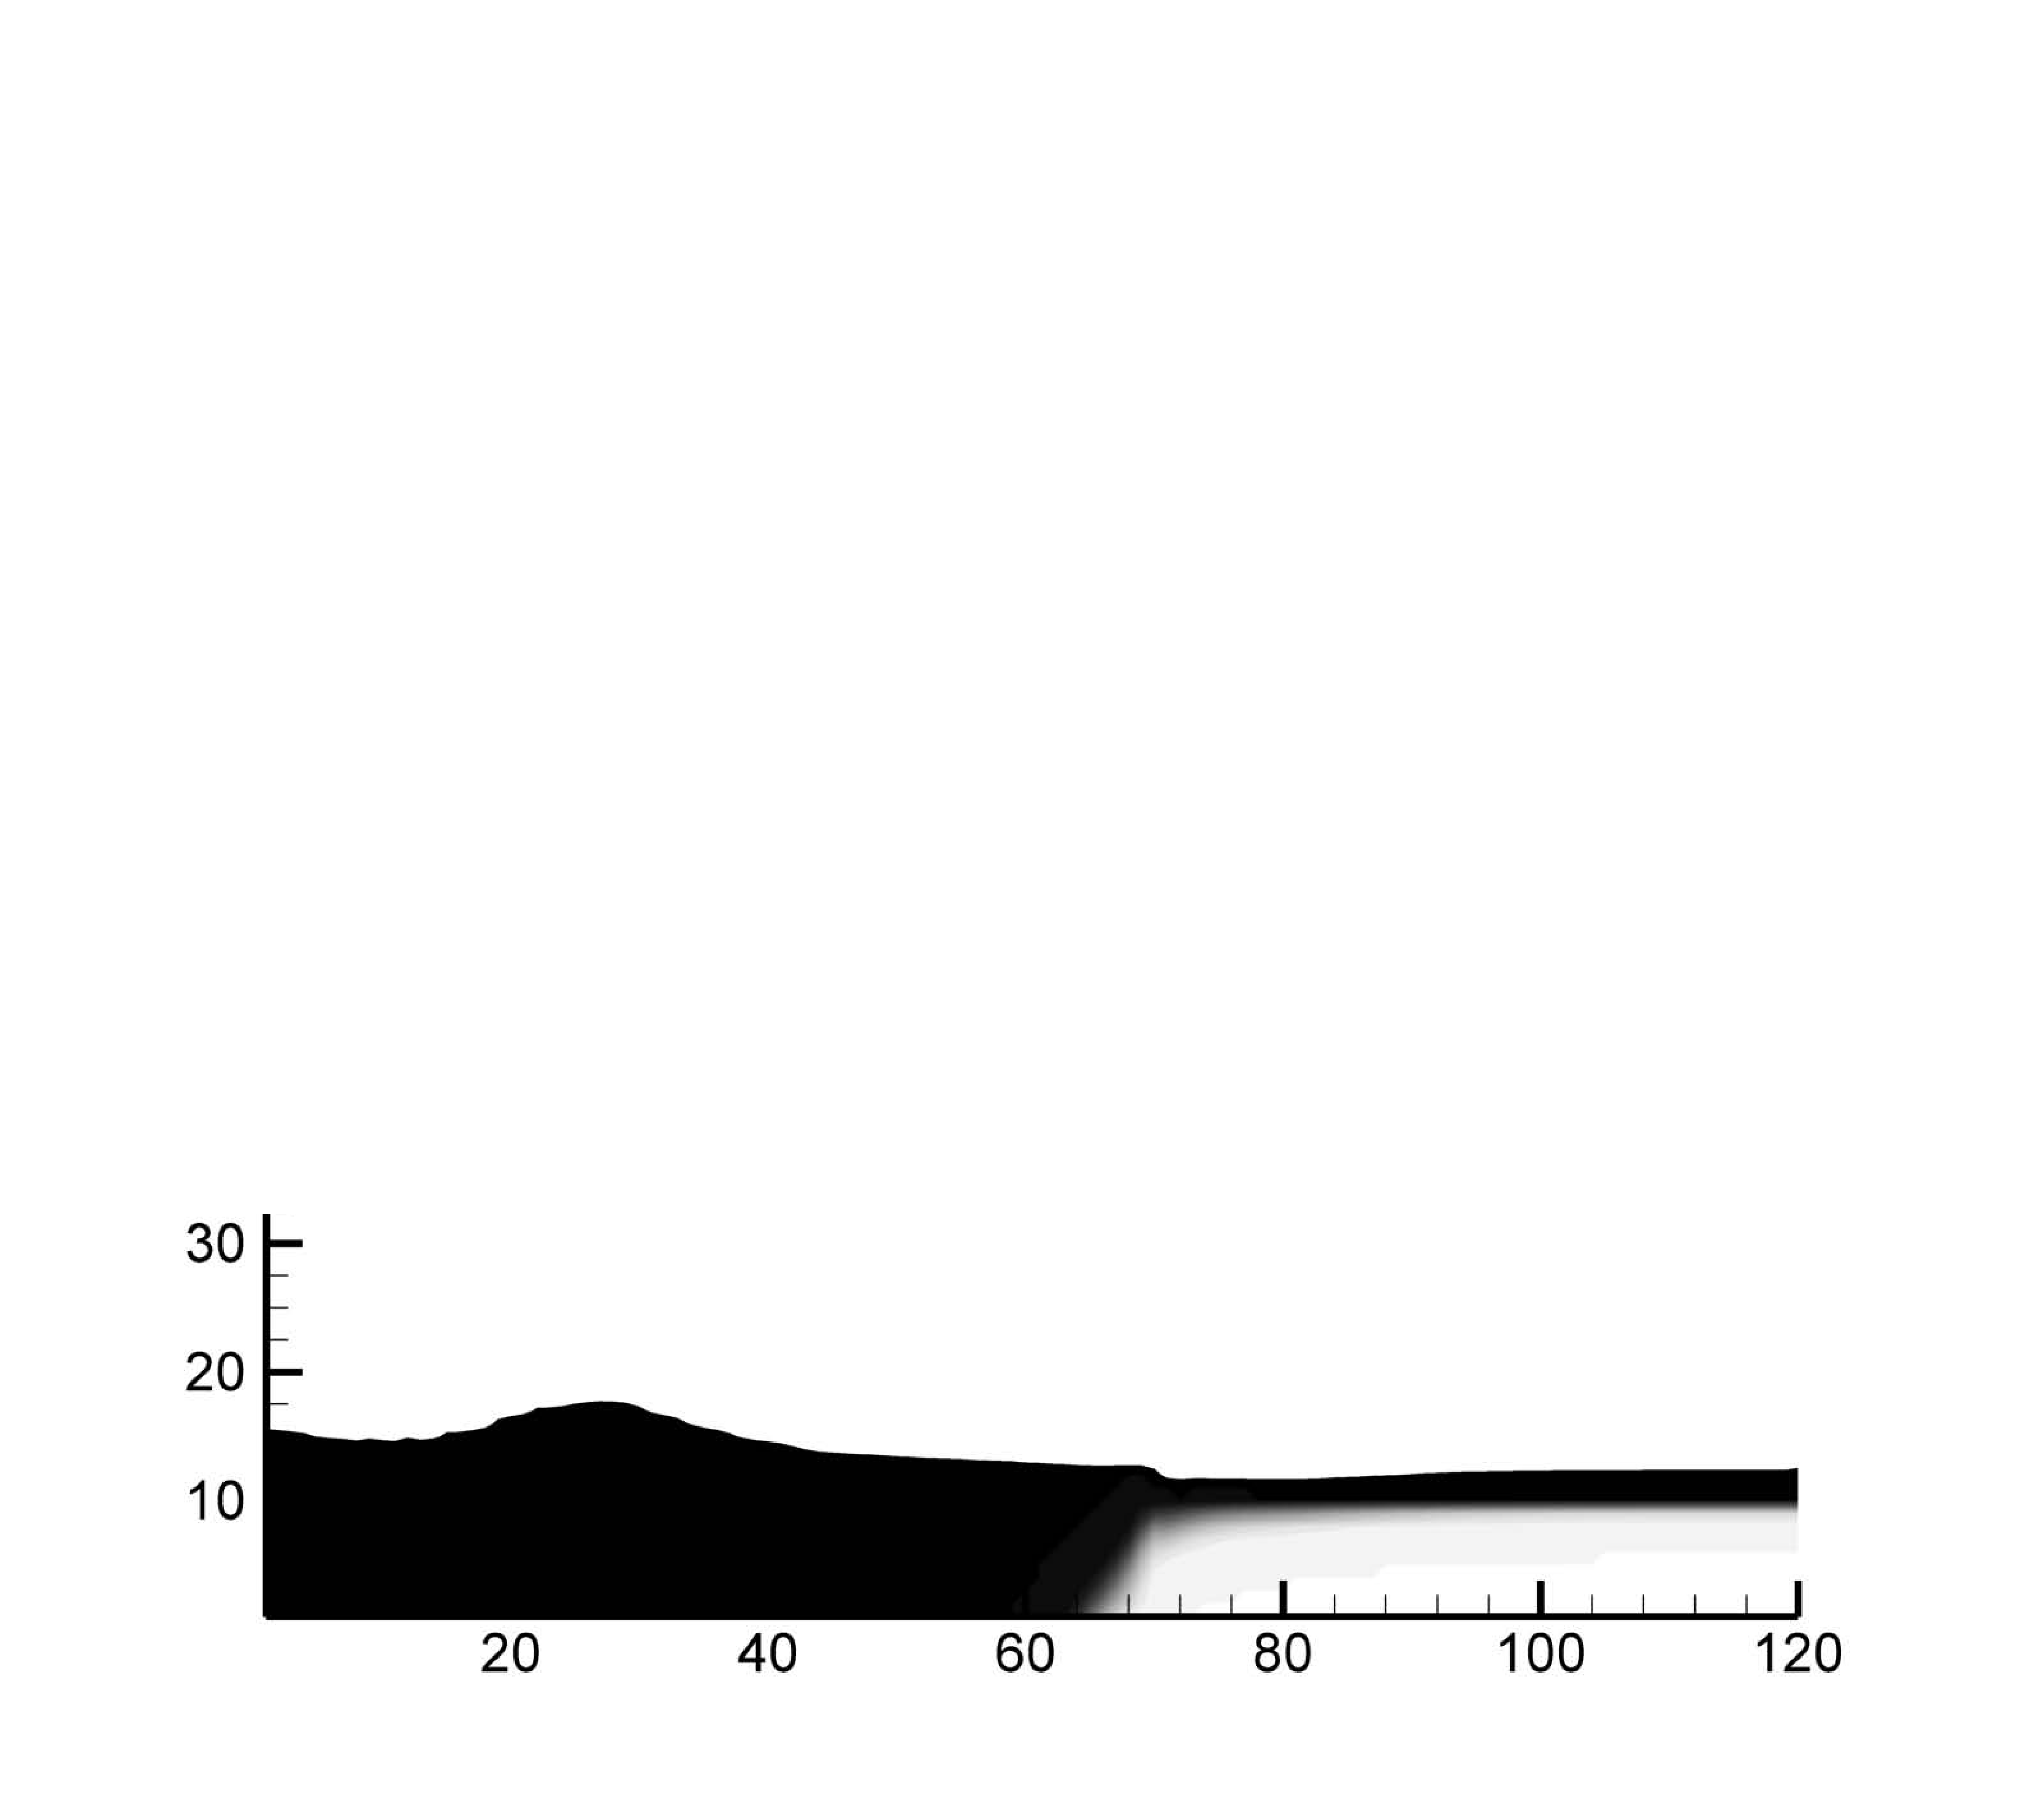
\includegraphics[width=3.5in]{../figures/SRM/025.pdf}
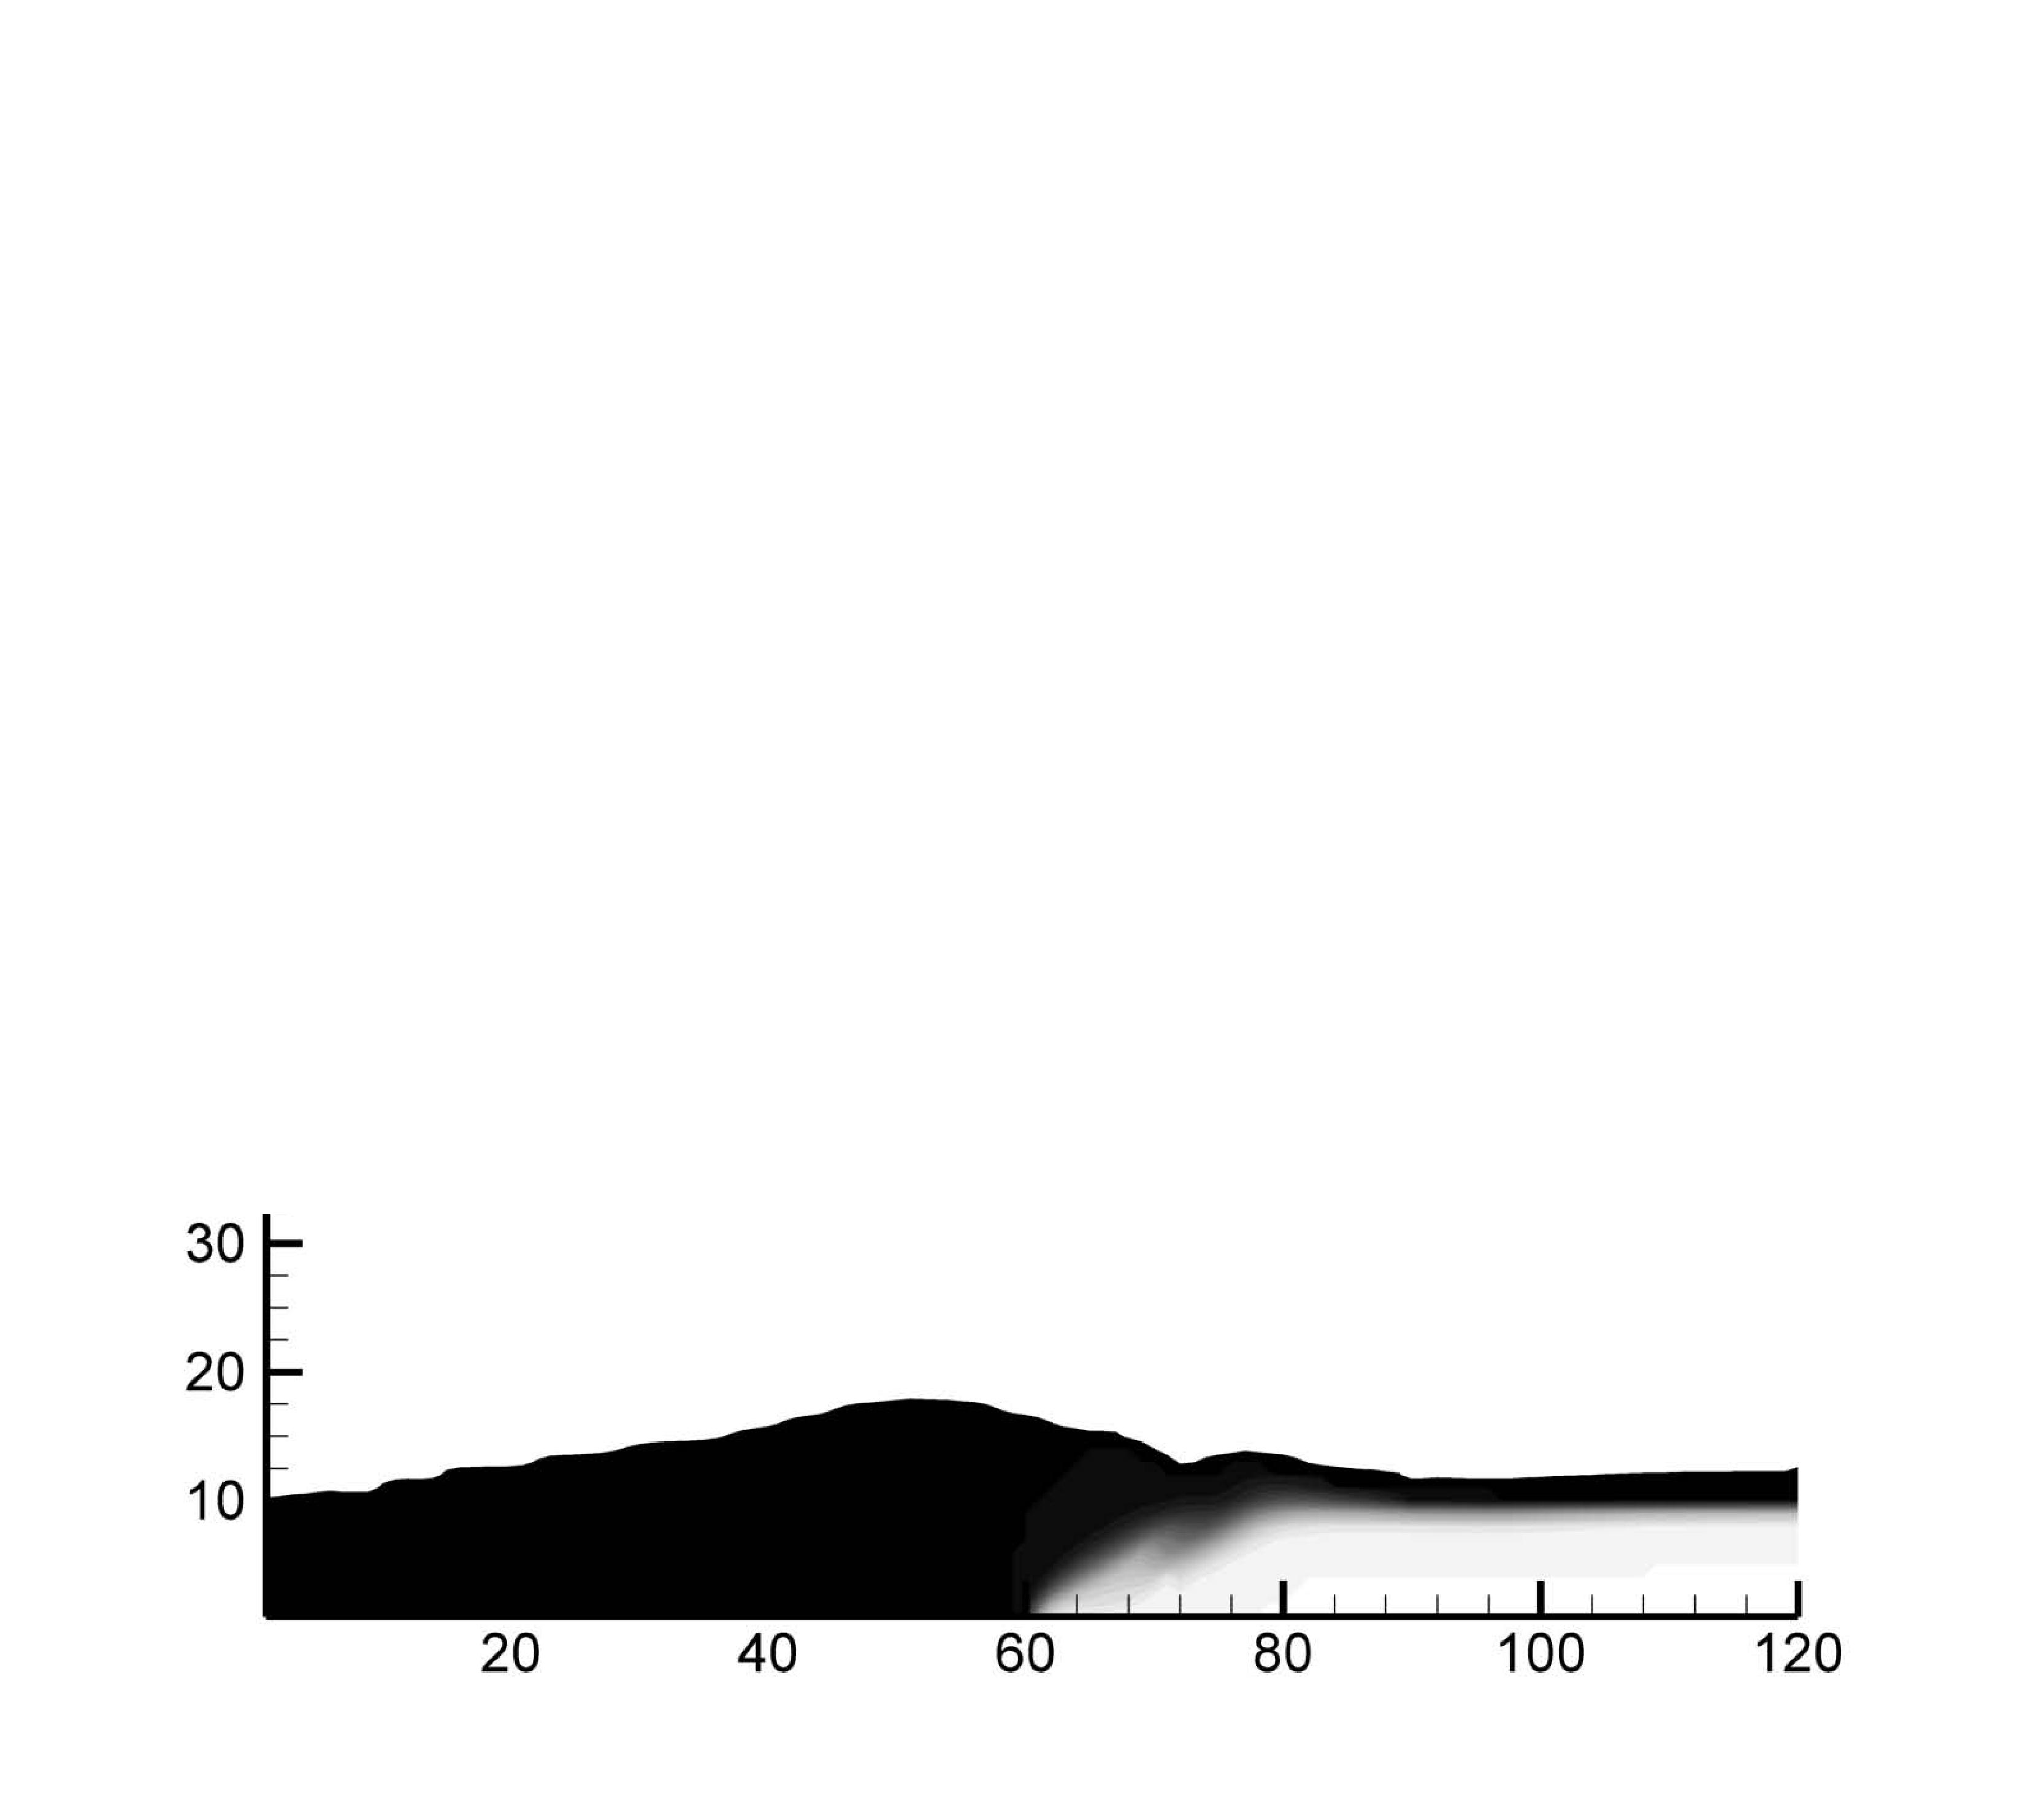
\includegraphics[width=3.5in]{../figures/SRM/050.pdf}
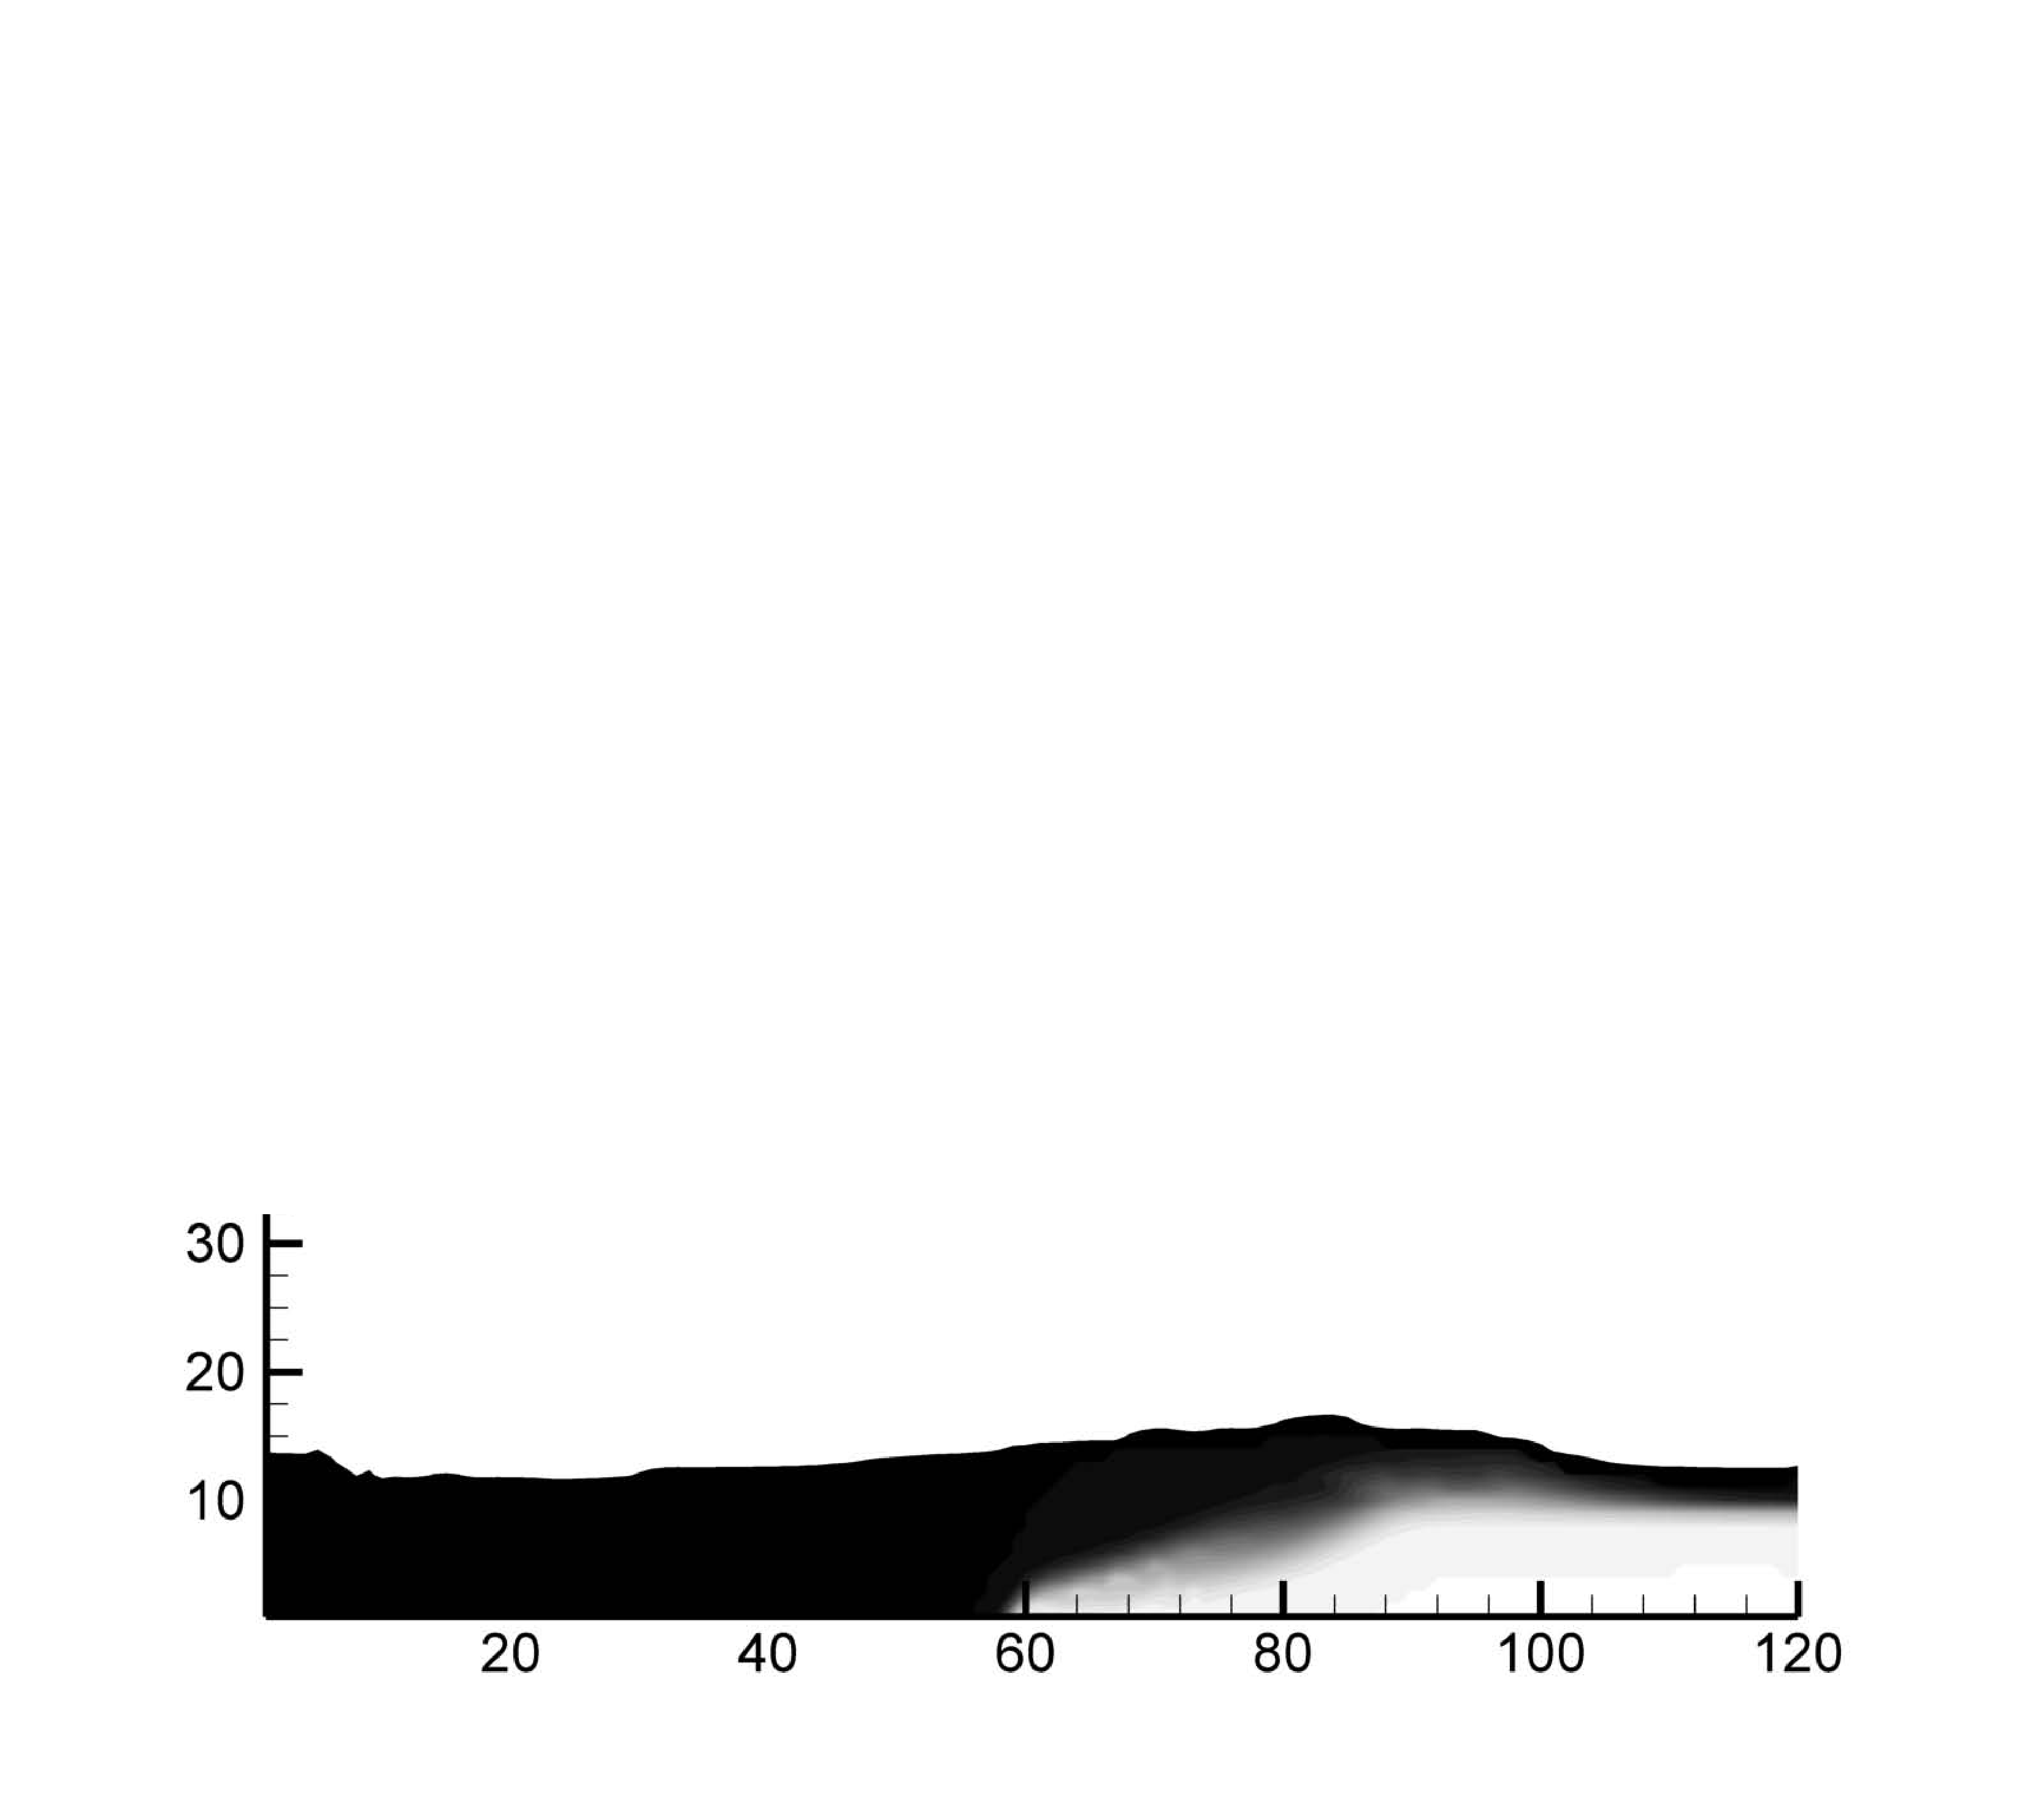
\includegraphics[width=3.5in]{../figures/SRM/075.pdf}
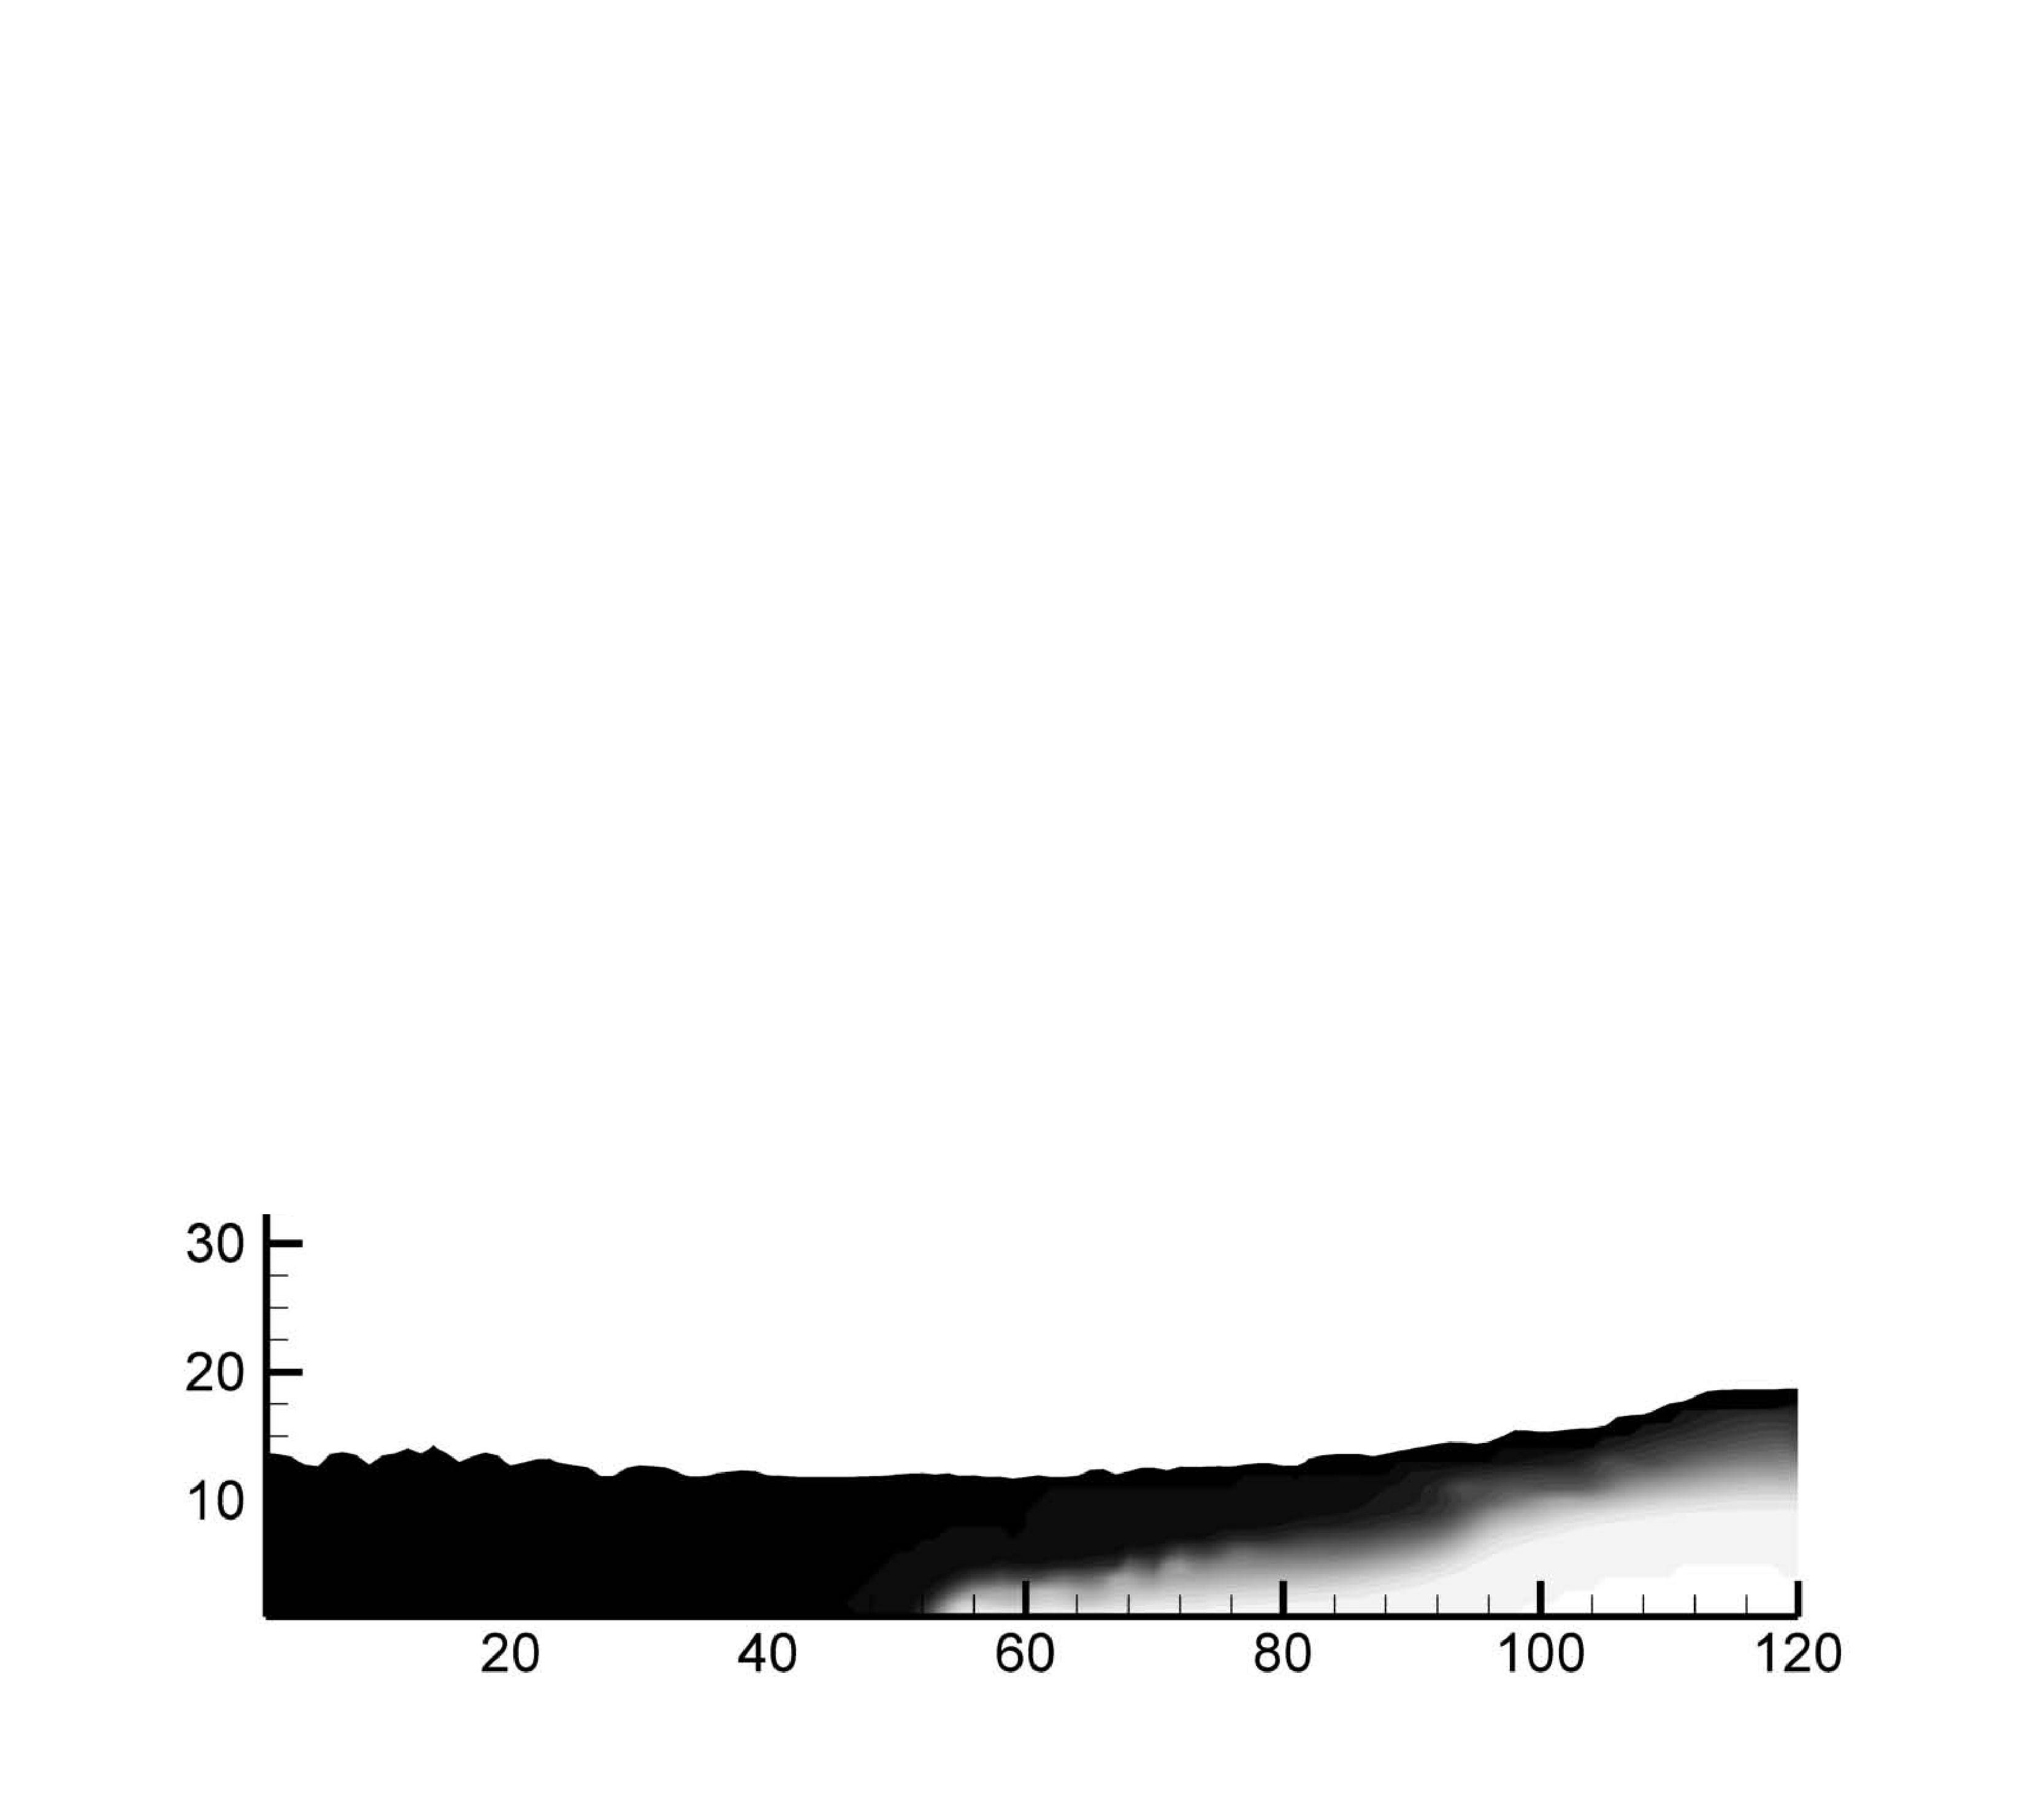
\includegraphics[width=3.5in]{../figures/SRM/100.pdf}
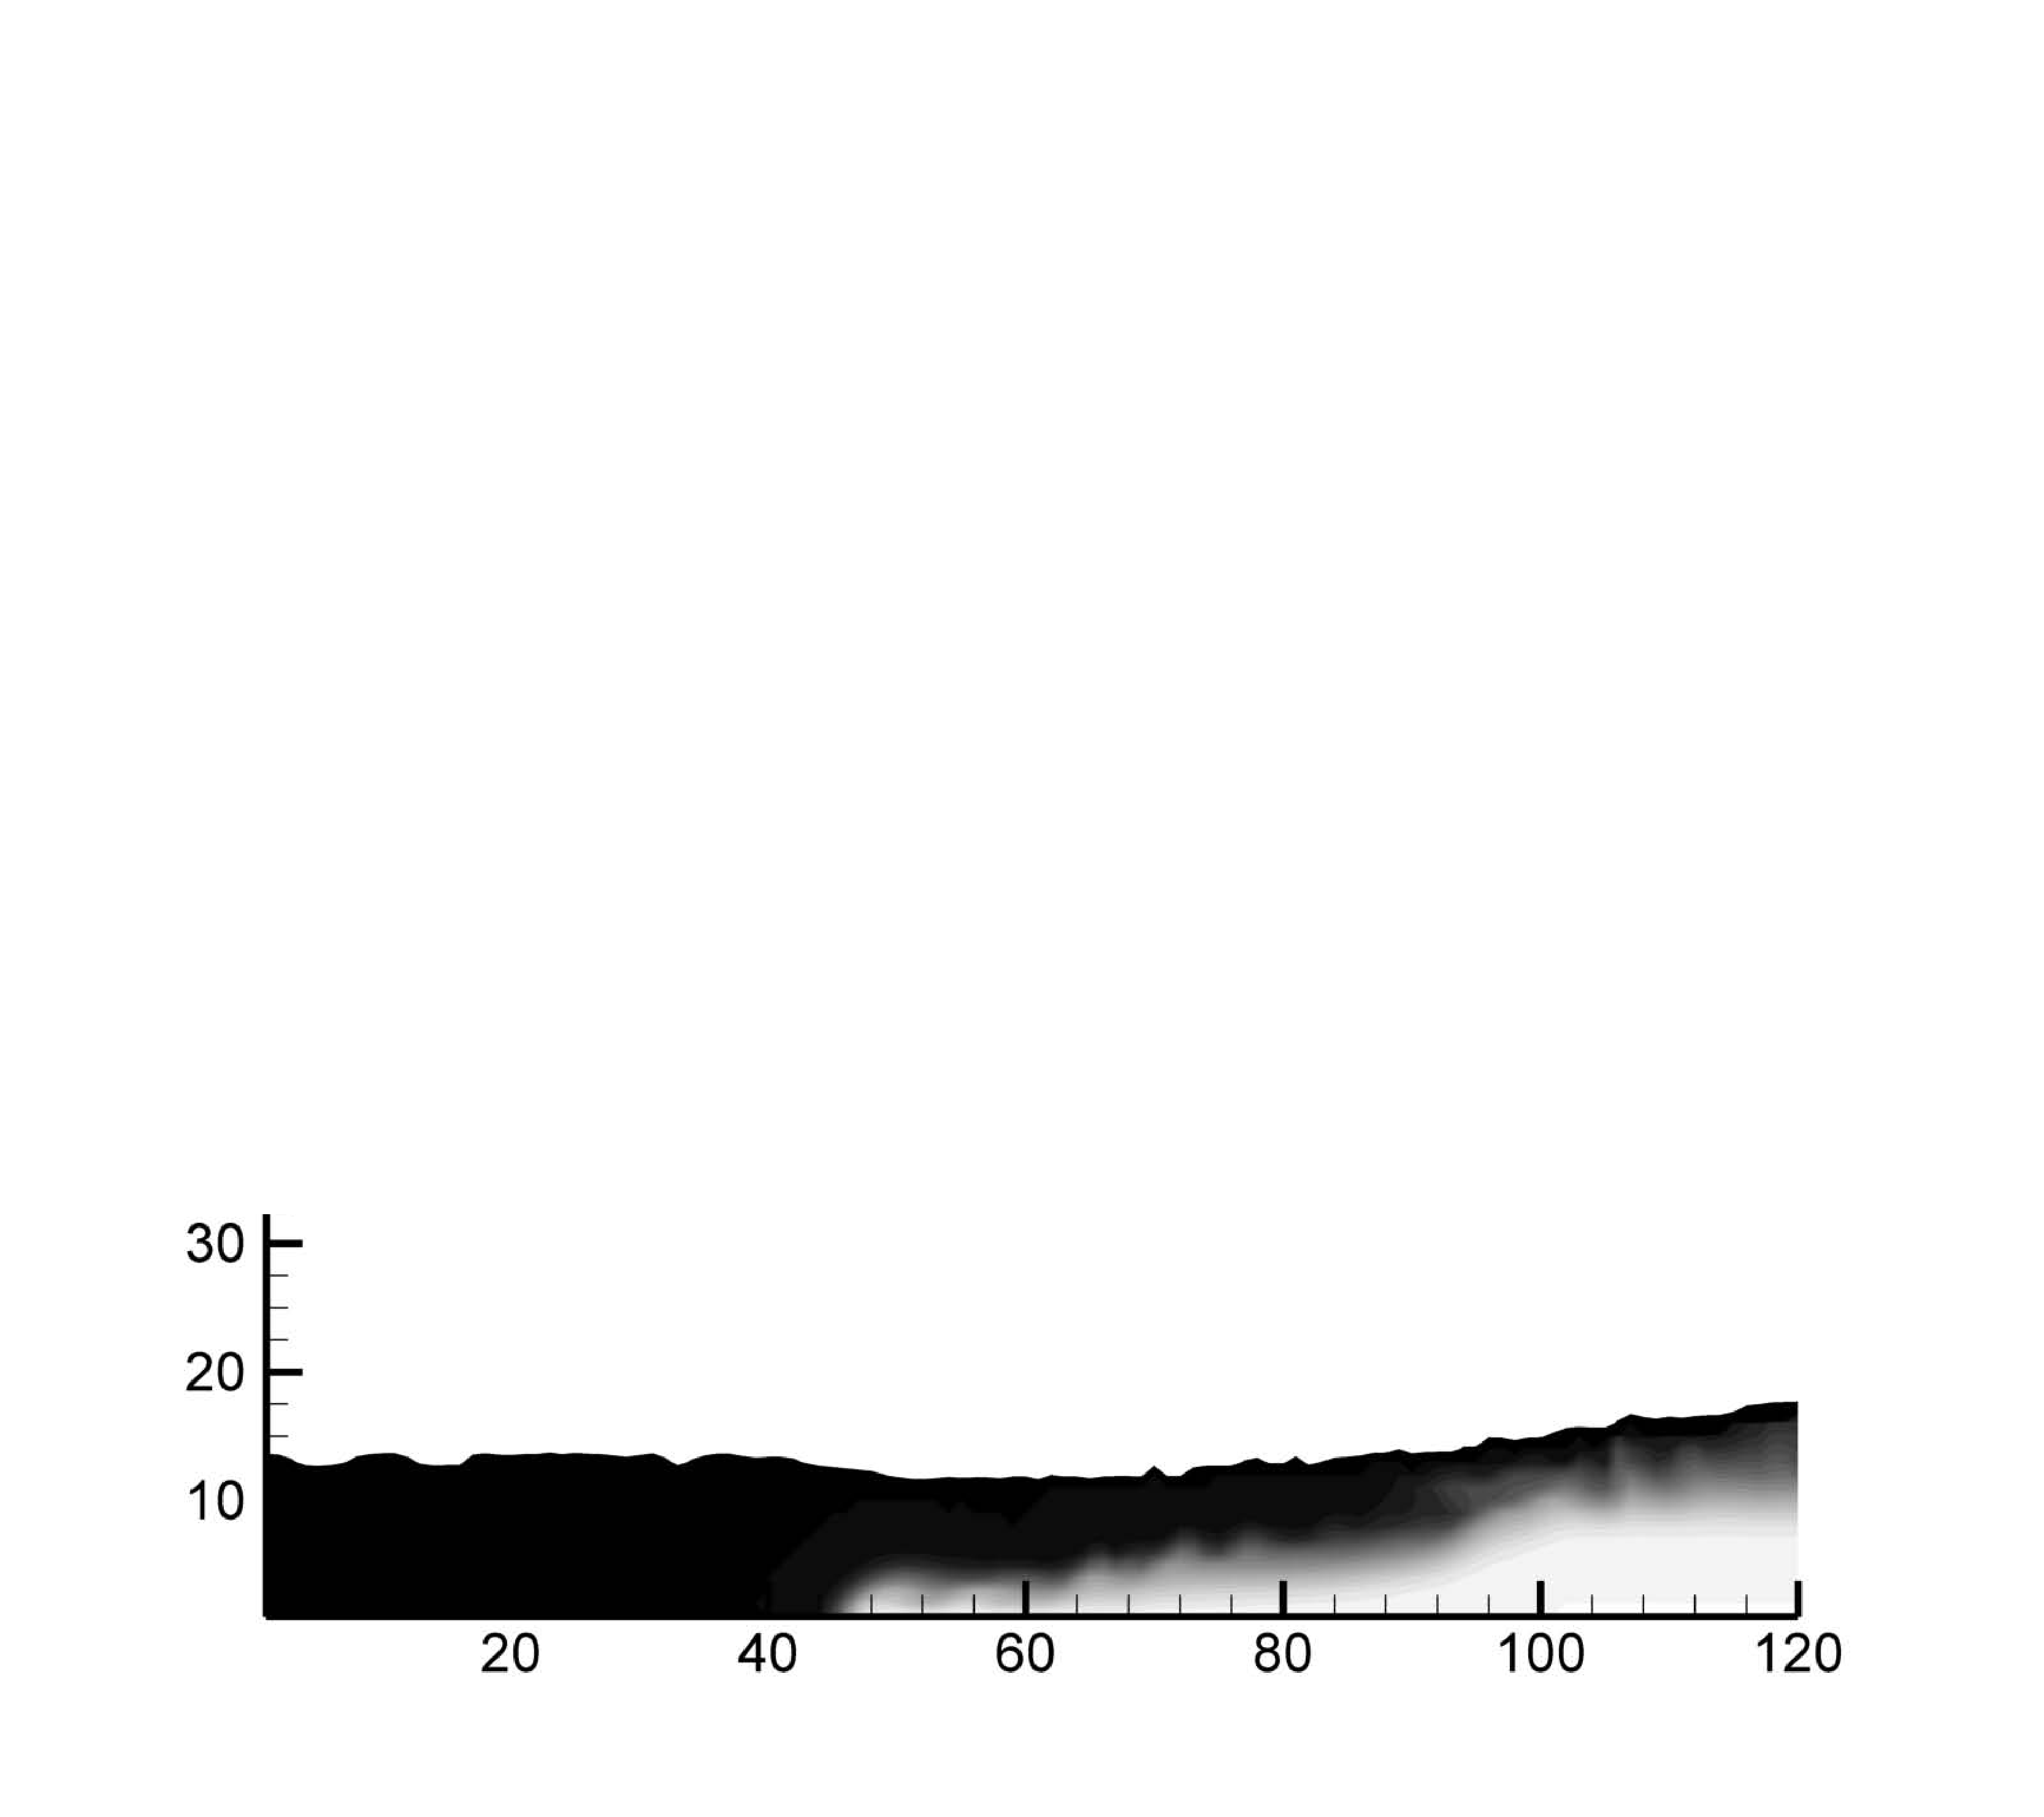
\includegraphics[width=3.5in]{../figures/SRM/125.pdf}
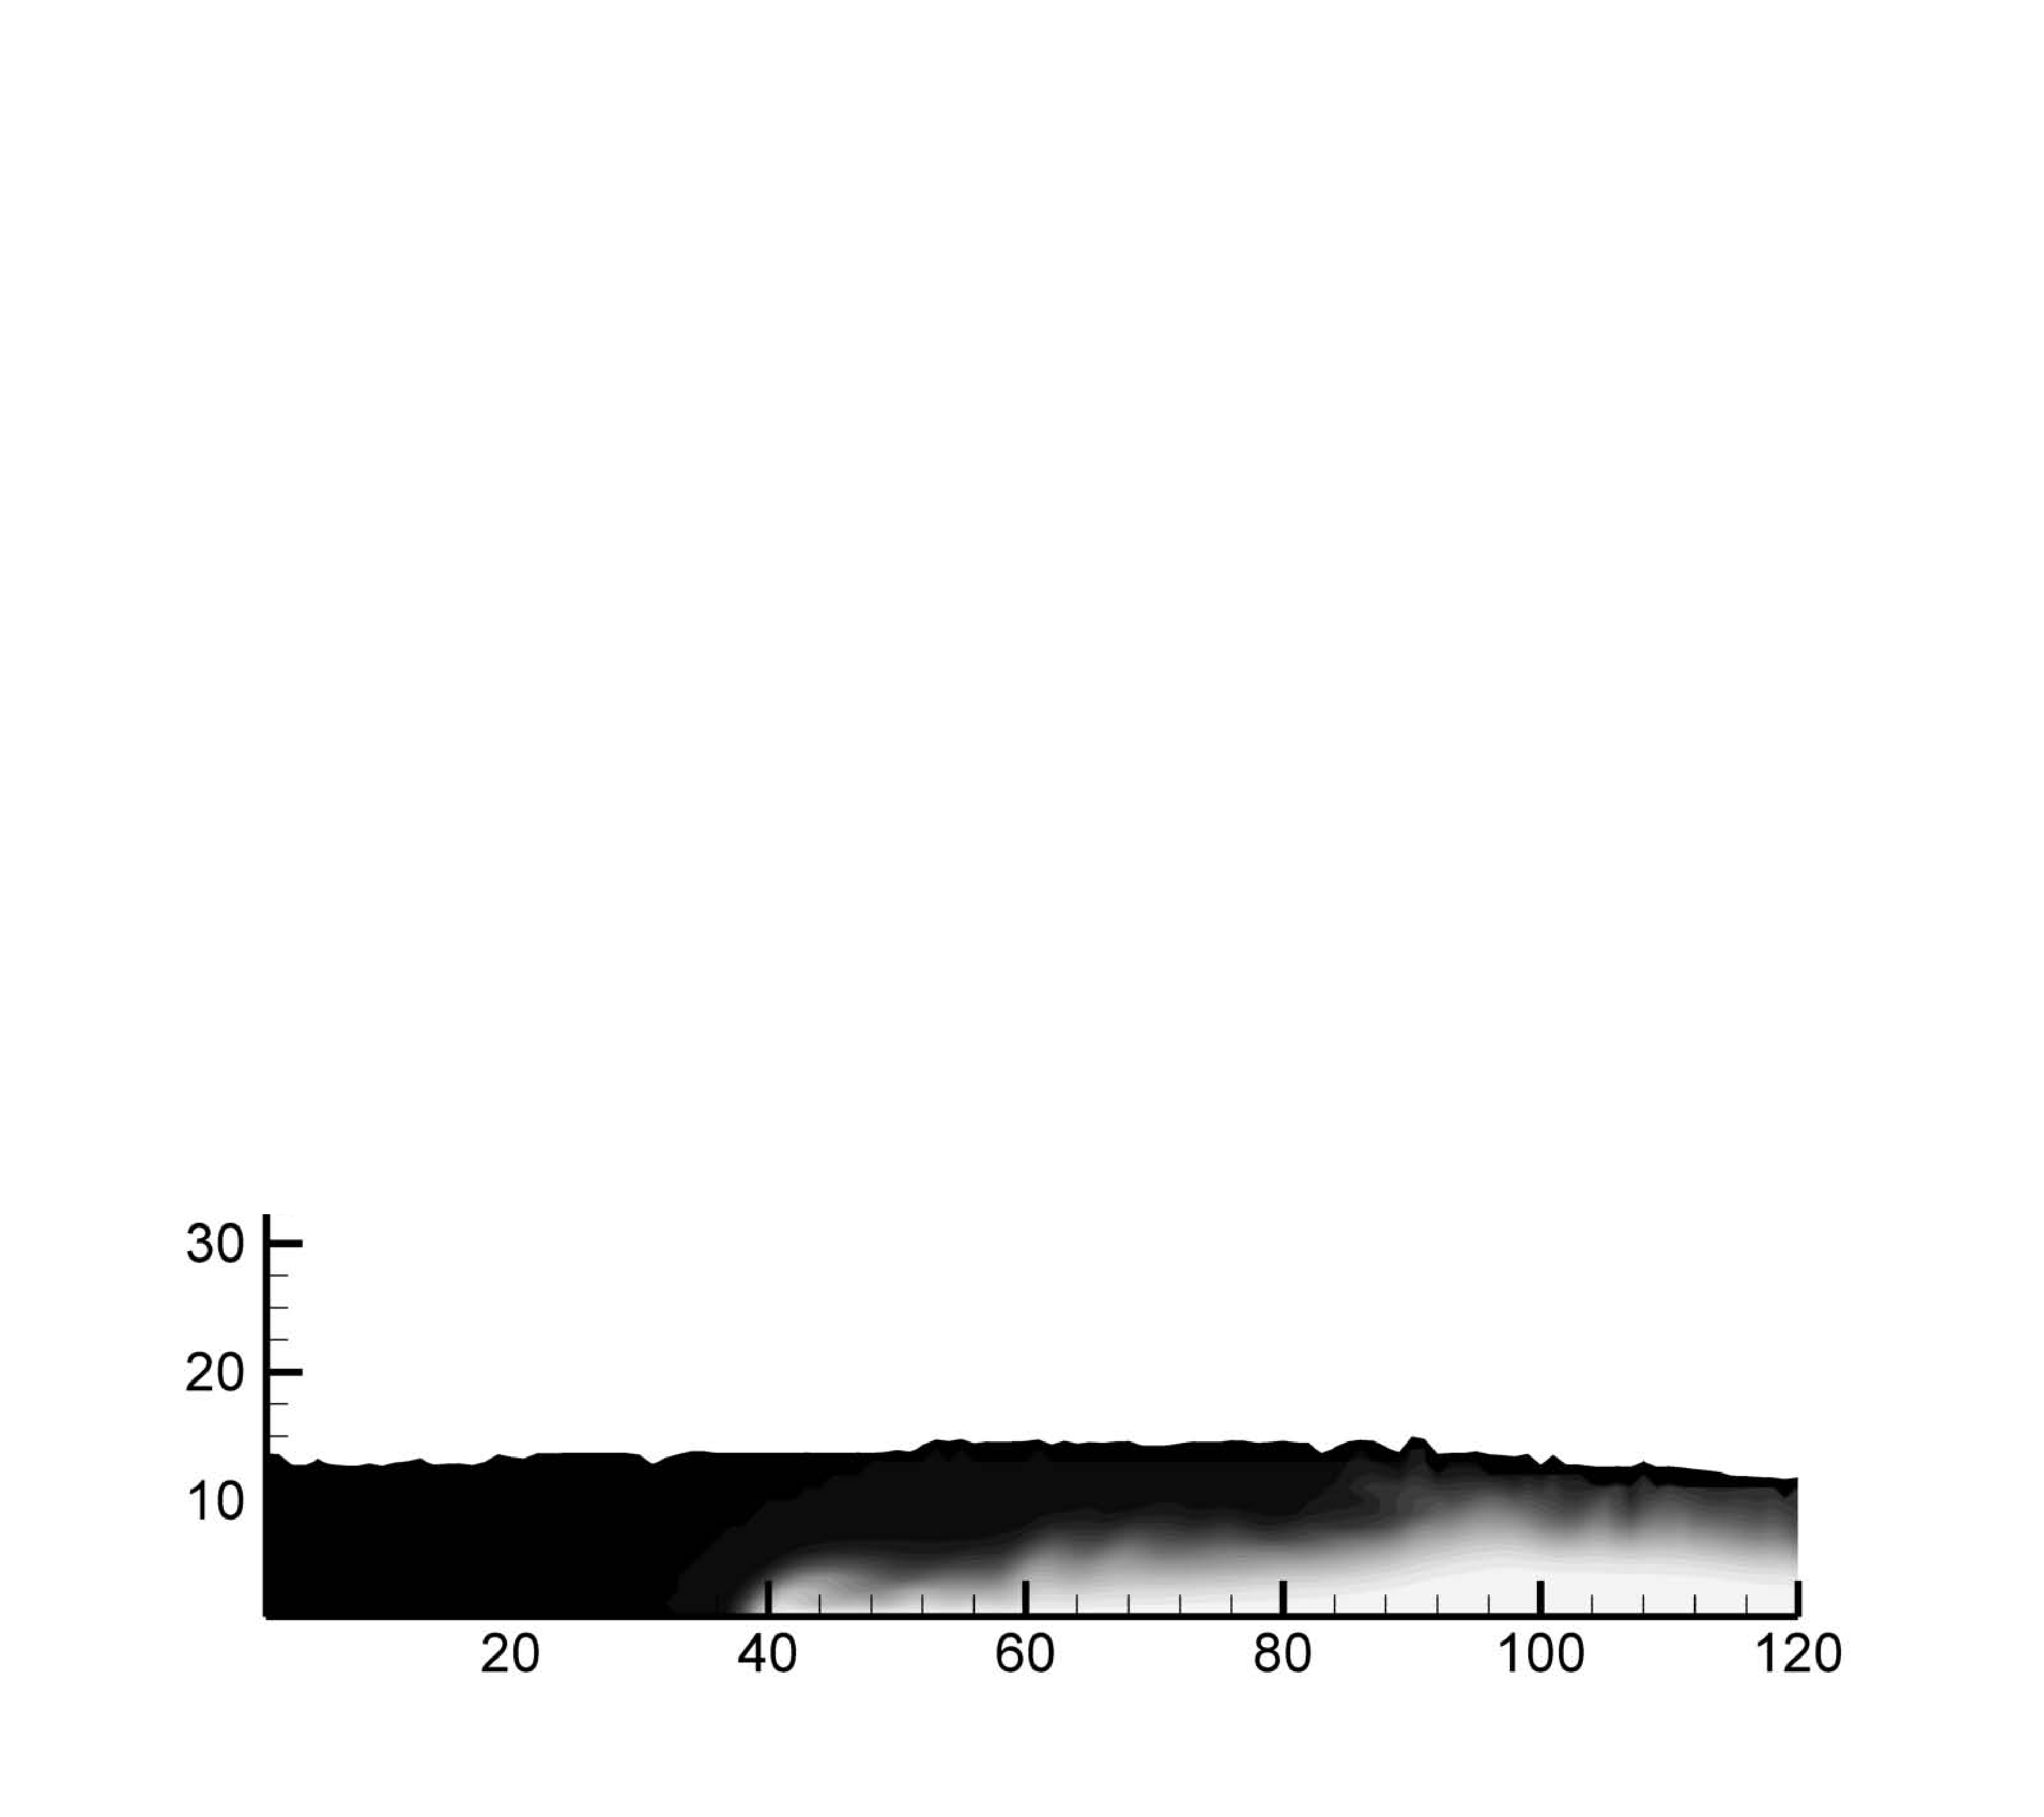
\includegraphics[width=3.5in]{../figures/SRM/150.pdf}
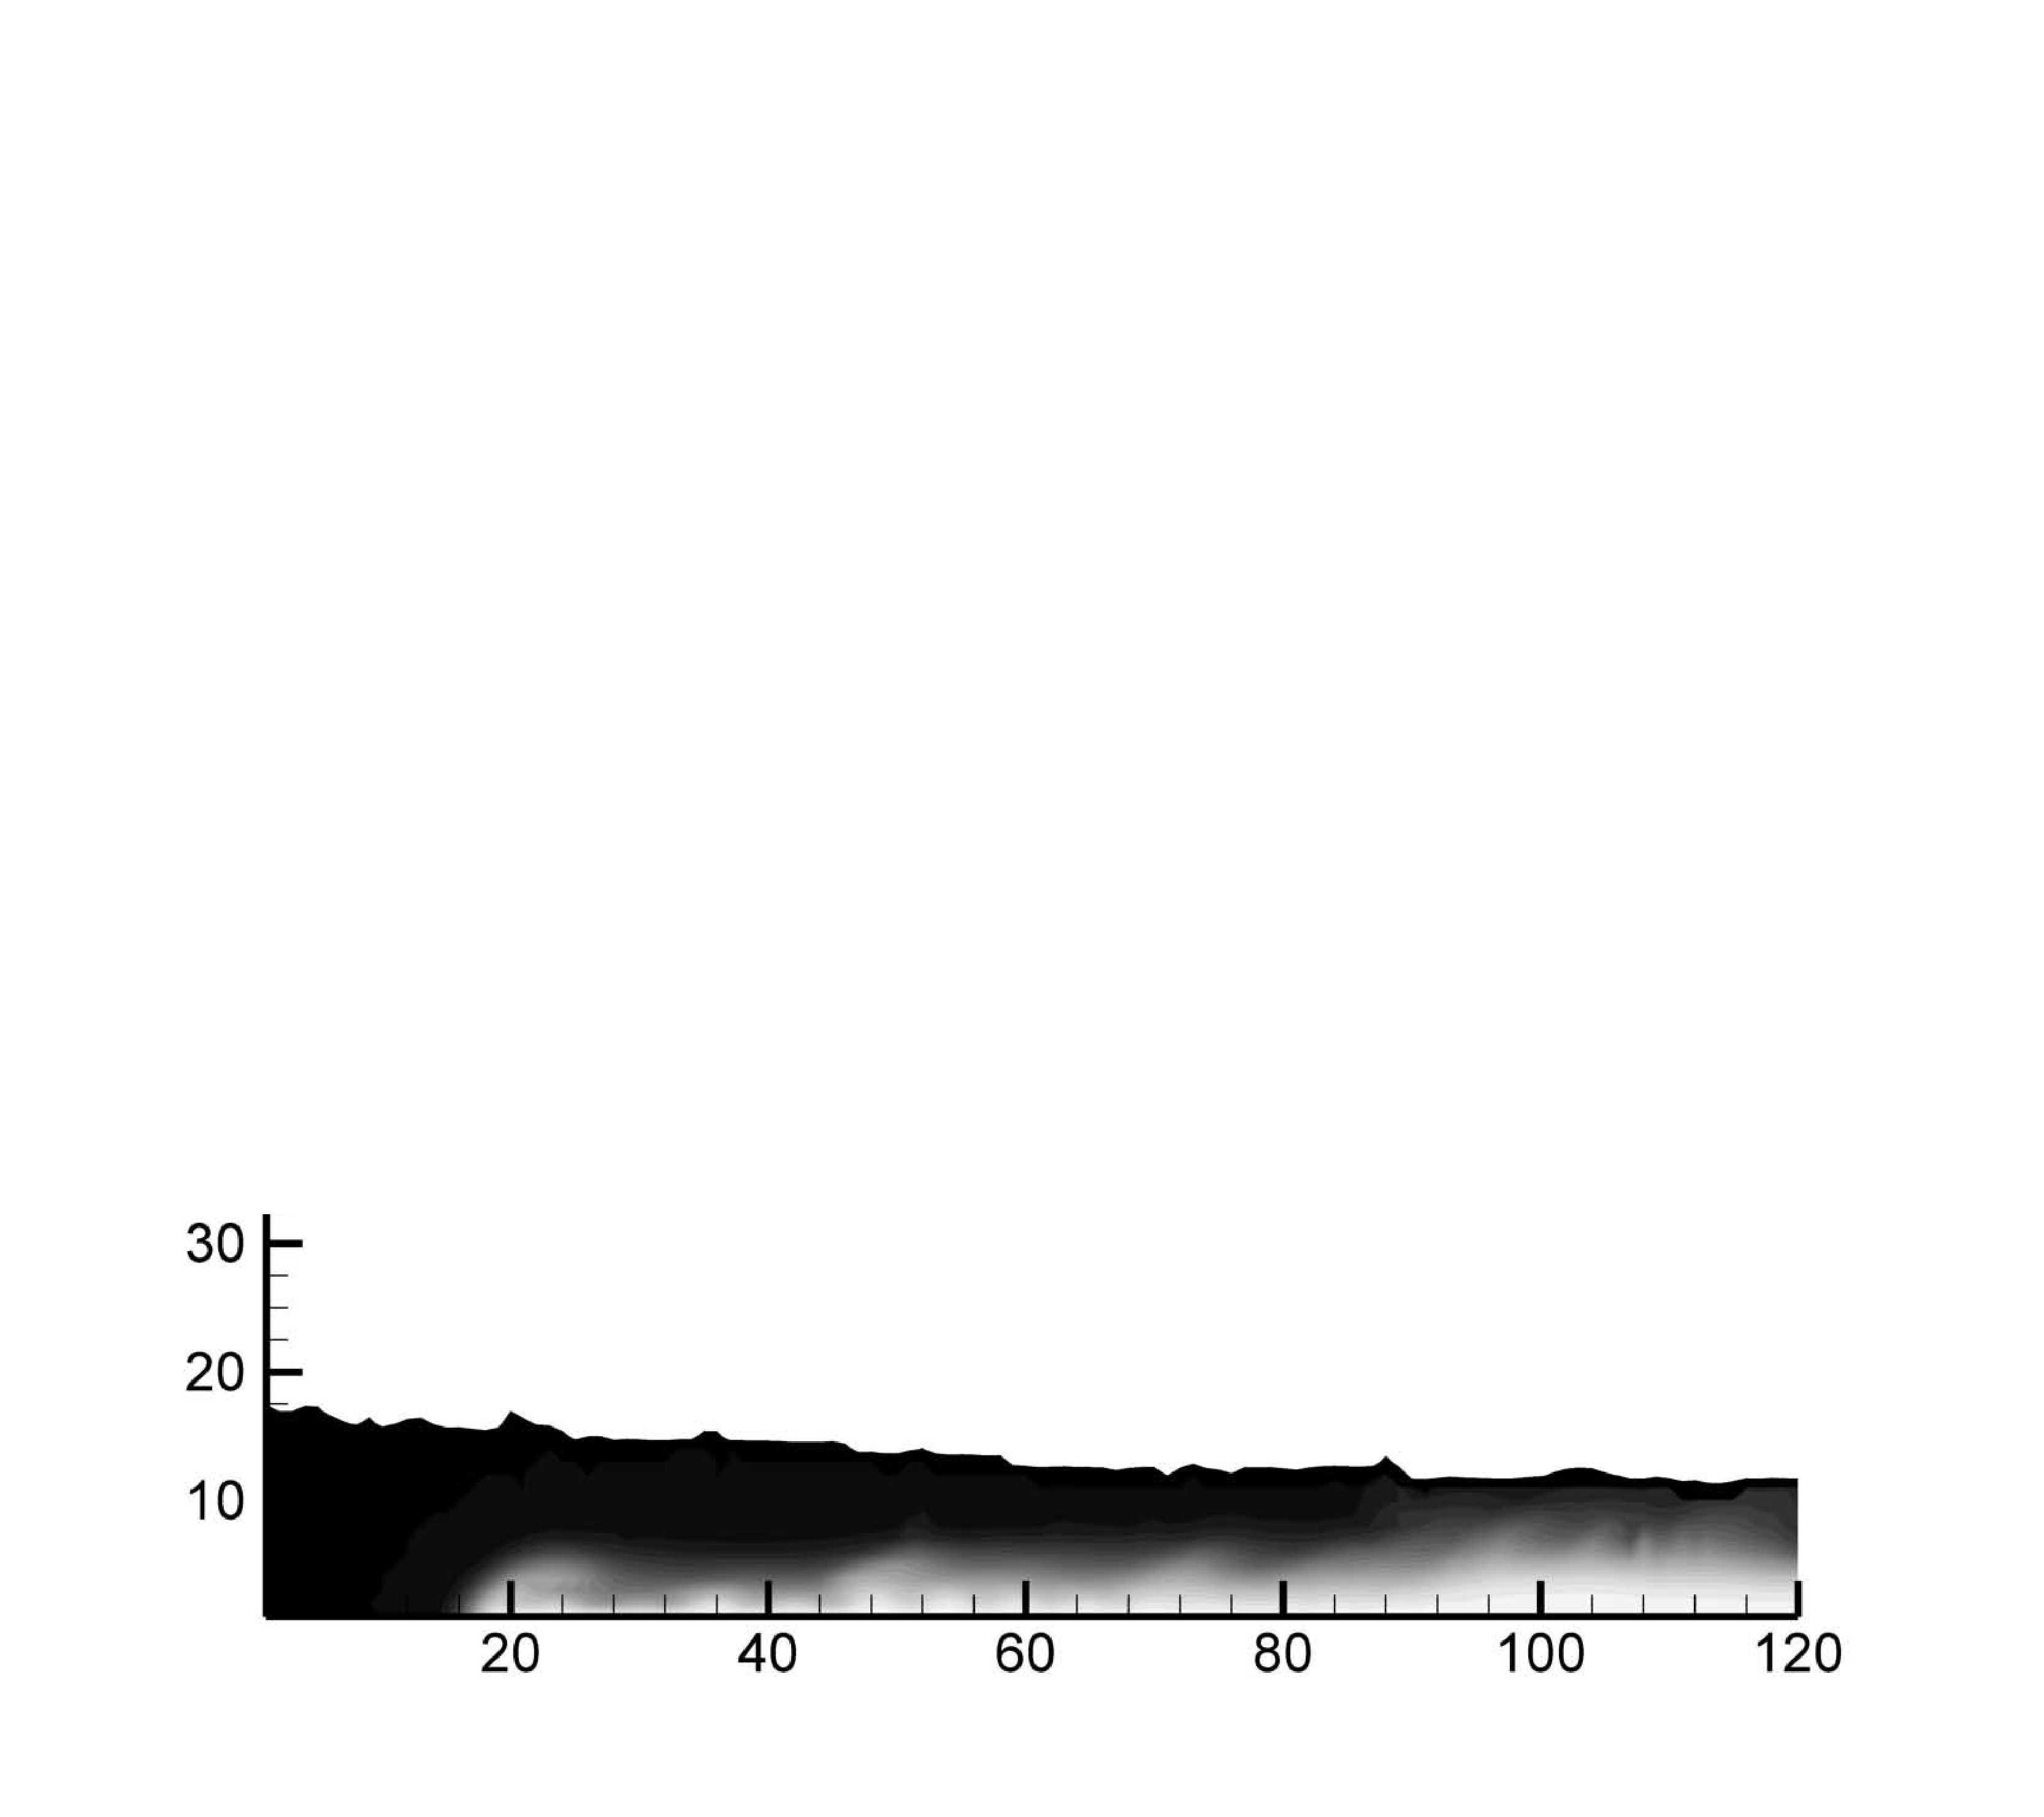
\includegraphics[width=3.5in]{../figures/SRM/200.pdf}
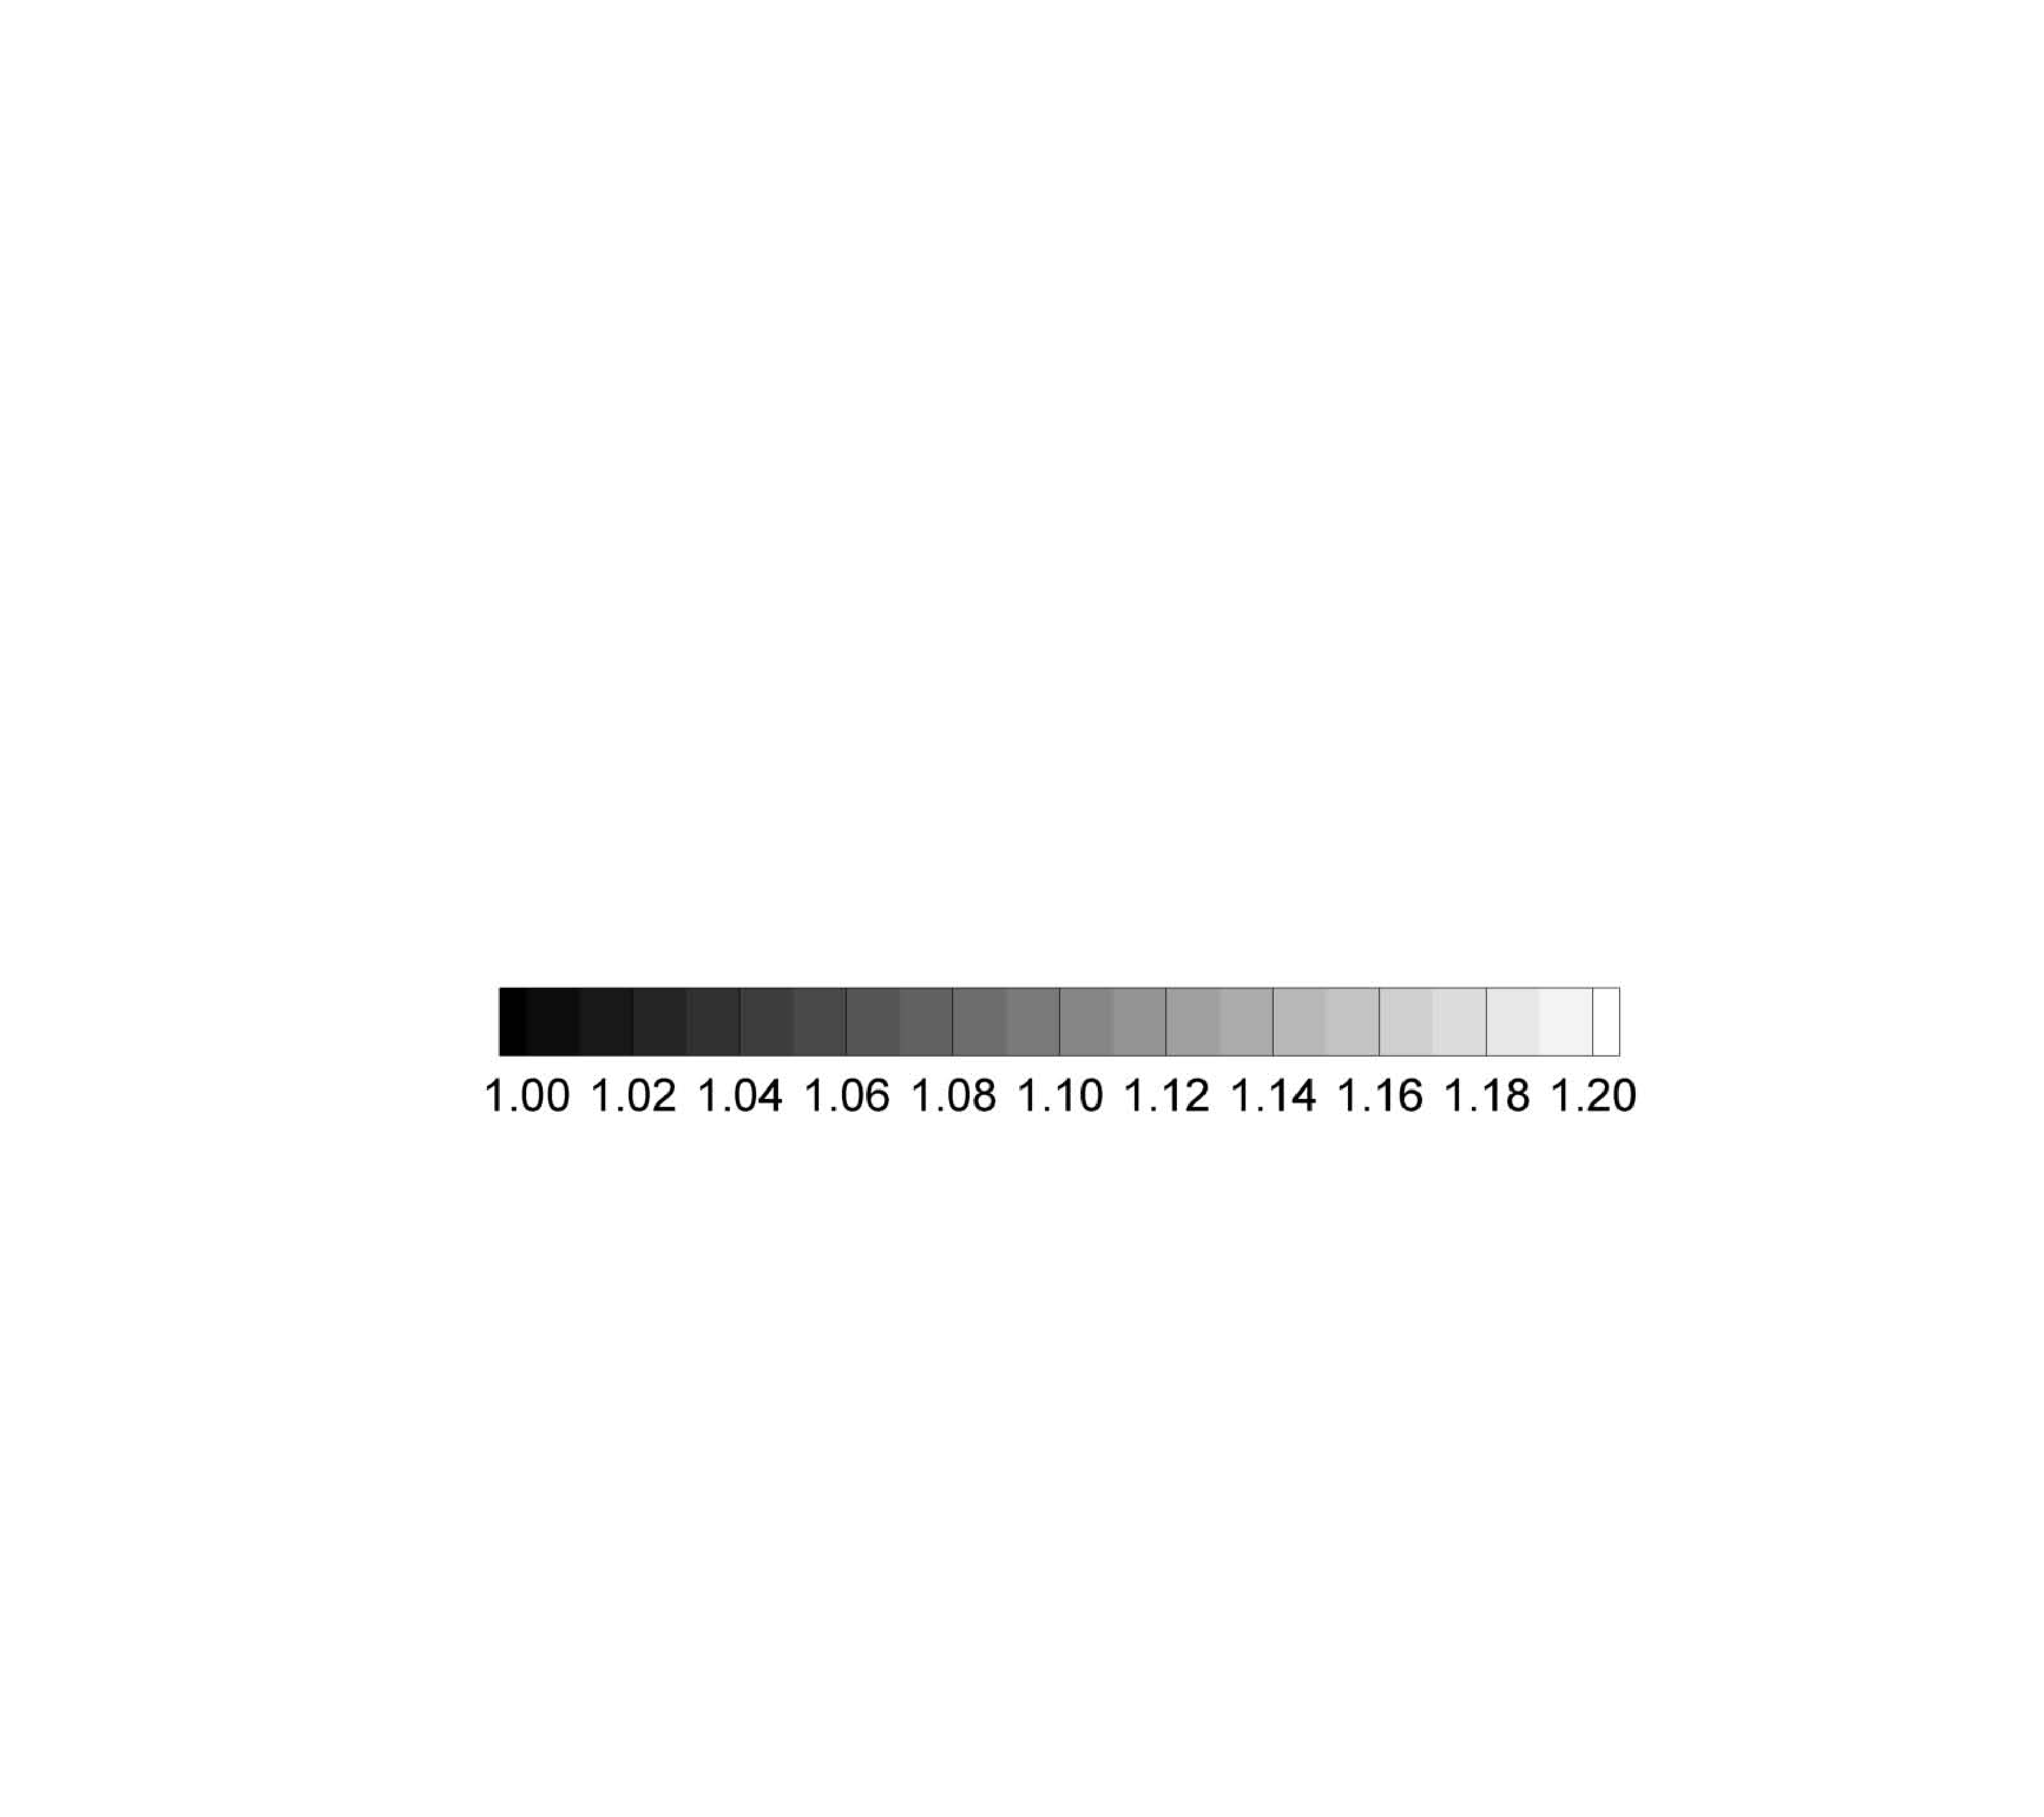
\includegraphics[width=3.0in]{../figures/SRM/contour.pdf}
\end{center}
    \caption{Projection method simulation results without domain decomposition.}
    \label{fig:Wave-GravityCurrent-Proj}
\end{figure}

\cp

\section{Summary}
A domain decomposition method is proposed for incompressible unsteady free-surface flow. An explicit sequential regularization method is used to solve incompressible Navier-Stokes equation on subdomain boundaries. The result from this explicit method provides subdomain boundary conditions for other implicit method inside each subdomain to advance to the next time step. An explicit scheme can be easily and fully parallelized, because the computation for the next time step requires only the previous time step information from neighboring nodes. However, they generally suffer from the severe time-step stability constraint of Courant-Friedrichs-Levy (CFL) number. An implicit scheme generally solves a system of equations either directly or iteratively, thus it cannot be parallelized as easily as an explicit scheme. However, it is not bounded by the severe time-step stability constraint. The explicit SRM method is tested with standing wave simulation and then the combination of explicit and implicit schemes is tested with the surface wave and gravity current simulations. The standing wave simulation results show that the explicit SRM still has room for research and optimization. The surface wave and gravity current test show that the explicit interface computation does transport both internal gravity current and external surface wave. This research inspired the development of receding boundary method in Chapter \ref{chapter:RBM}.



